\documentclass{beamer}
\input{../style/cours-style.sty}

% Title
\title[LINUX2]{Linux - Avancé pour Administrateur/PowerUser - LINUX2}
\author{Christophe Brun}
\institute{Digicomp}
\date{17 avril 2024}
\beamertemplatenavigationsymbolsempty

\titlegraphic{
    \bigbreak
    
\includegraphics[width=5cm]{image/digicomp-logo}
    \bigbreak
    Digital competence. Made of People.
    \bigbreak
}

\begin{document}

    \begin{frame}
        \titlepage
    \end{frame}


    \section{Table des matières}\label{sec:toc}

    \begin{frame}{Table des matières}
        \begin{tiny}
            \begin{multicols}{2}
                \tableofcontents
            \end{multicols}
        \end{tiny}
    \end{frame}


    \section{Programme du module}\label{sec:programme-du-module}

    \begin{frame}{Linux - Avancé pour Administrateur/PowerUser}{Objectifs des 4 jours}
        \begin{columns}
            \column{0.7\textwidth}
            \begin{scriptsize}
                \begin{itemize}
                    \item Connaître l'architecture Linux
                    \item Travailler avec des commandes avancées dans le terminal
                    \item Utiliser les commandes de filtre (\lstinline{sed}, \lstinline{grep}, \lstinline{awk}, \textit{etc}.)
                    \item Gérer les utilisateurs et groupes
                    \item Définir et modifier les autorisations
                    \item Appliquer des privilèges personnalisés
                    \item Créer, gérer et exploiter des systèmes de fichiers
                    \item Créer, gérer et surveiller des processus
                    \item Connaître les services Unix
                    \item Automatiser les tâches de maintenance (\lstinline{cron}, \lstinline{at})
                    \item Installer des logiciels
                    \item Compiler des logiciels
                    \item Connaître Shell comme langage de programmation
                    \item Concevoir et écrire vos propres petits scripts Shell
                \end{itemize}
            \end{scriptsize}
            \column{0.3\textwidth}
            
\includegraphics[width=4cm]{image/IT-man-and-penguin}
        \end{columns}
    \end{frame}


    \section{Introduction}\label{sec:introduction}

    \begin{frame}{Formateur sur Linux}{Christophe Brun, conseil en développement informatique}

        \begin{columns}
            \column{0.7\textwidth}
            \begin{itemize}
                \item Développeur freelance (Python, Java, CoBOL) et data at scale.

                \item 7 ans de conseil en développement au sein d'SSII~.

                \item 7 ans de conseil en développement en indépendant, \href{https://papit.fr}{PapIT}.

                \item Passionné~!
                \bigbreak
                \begin{columns}
                    \column{0.5\textwidth}
                    \centering
                    
\includegraphics[width=3cm]{image/logo-uppa}
                    \column{0.5\textwidth}
                    \centering
                    
\includegraphics[width=3cm]{image/logo-universite-bordeaux}
                \end{columns}
            \end{itemize}
            \column{0.3\textwidth}
            \centering
            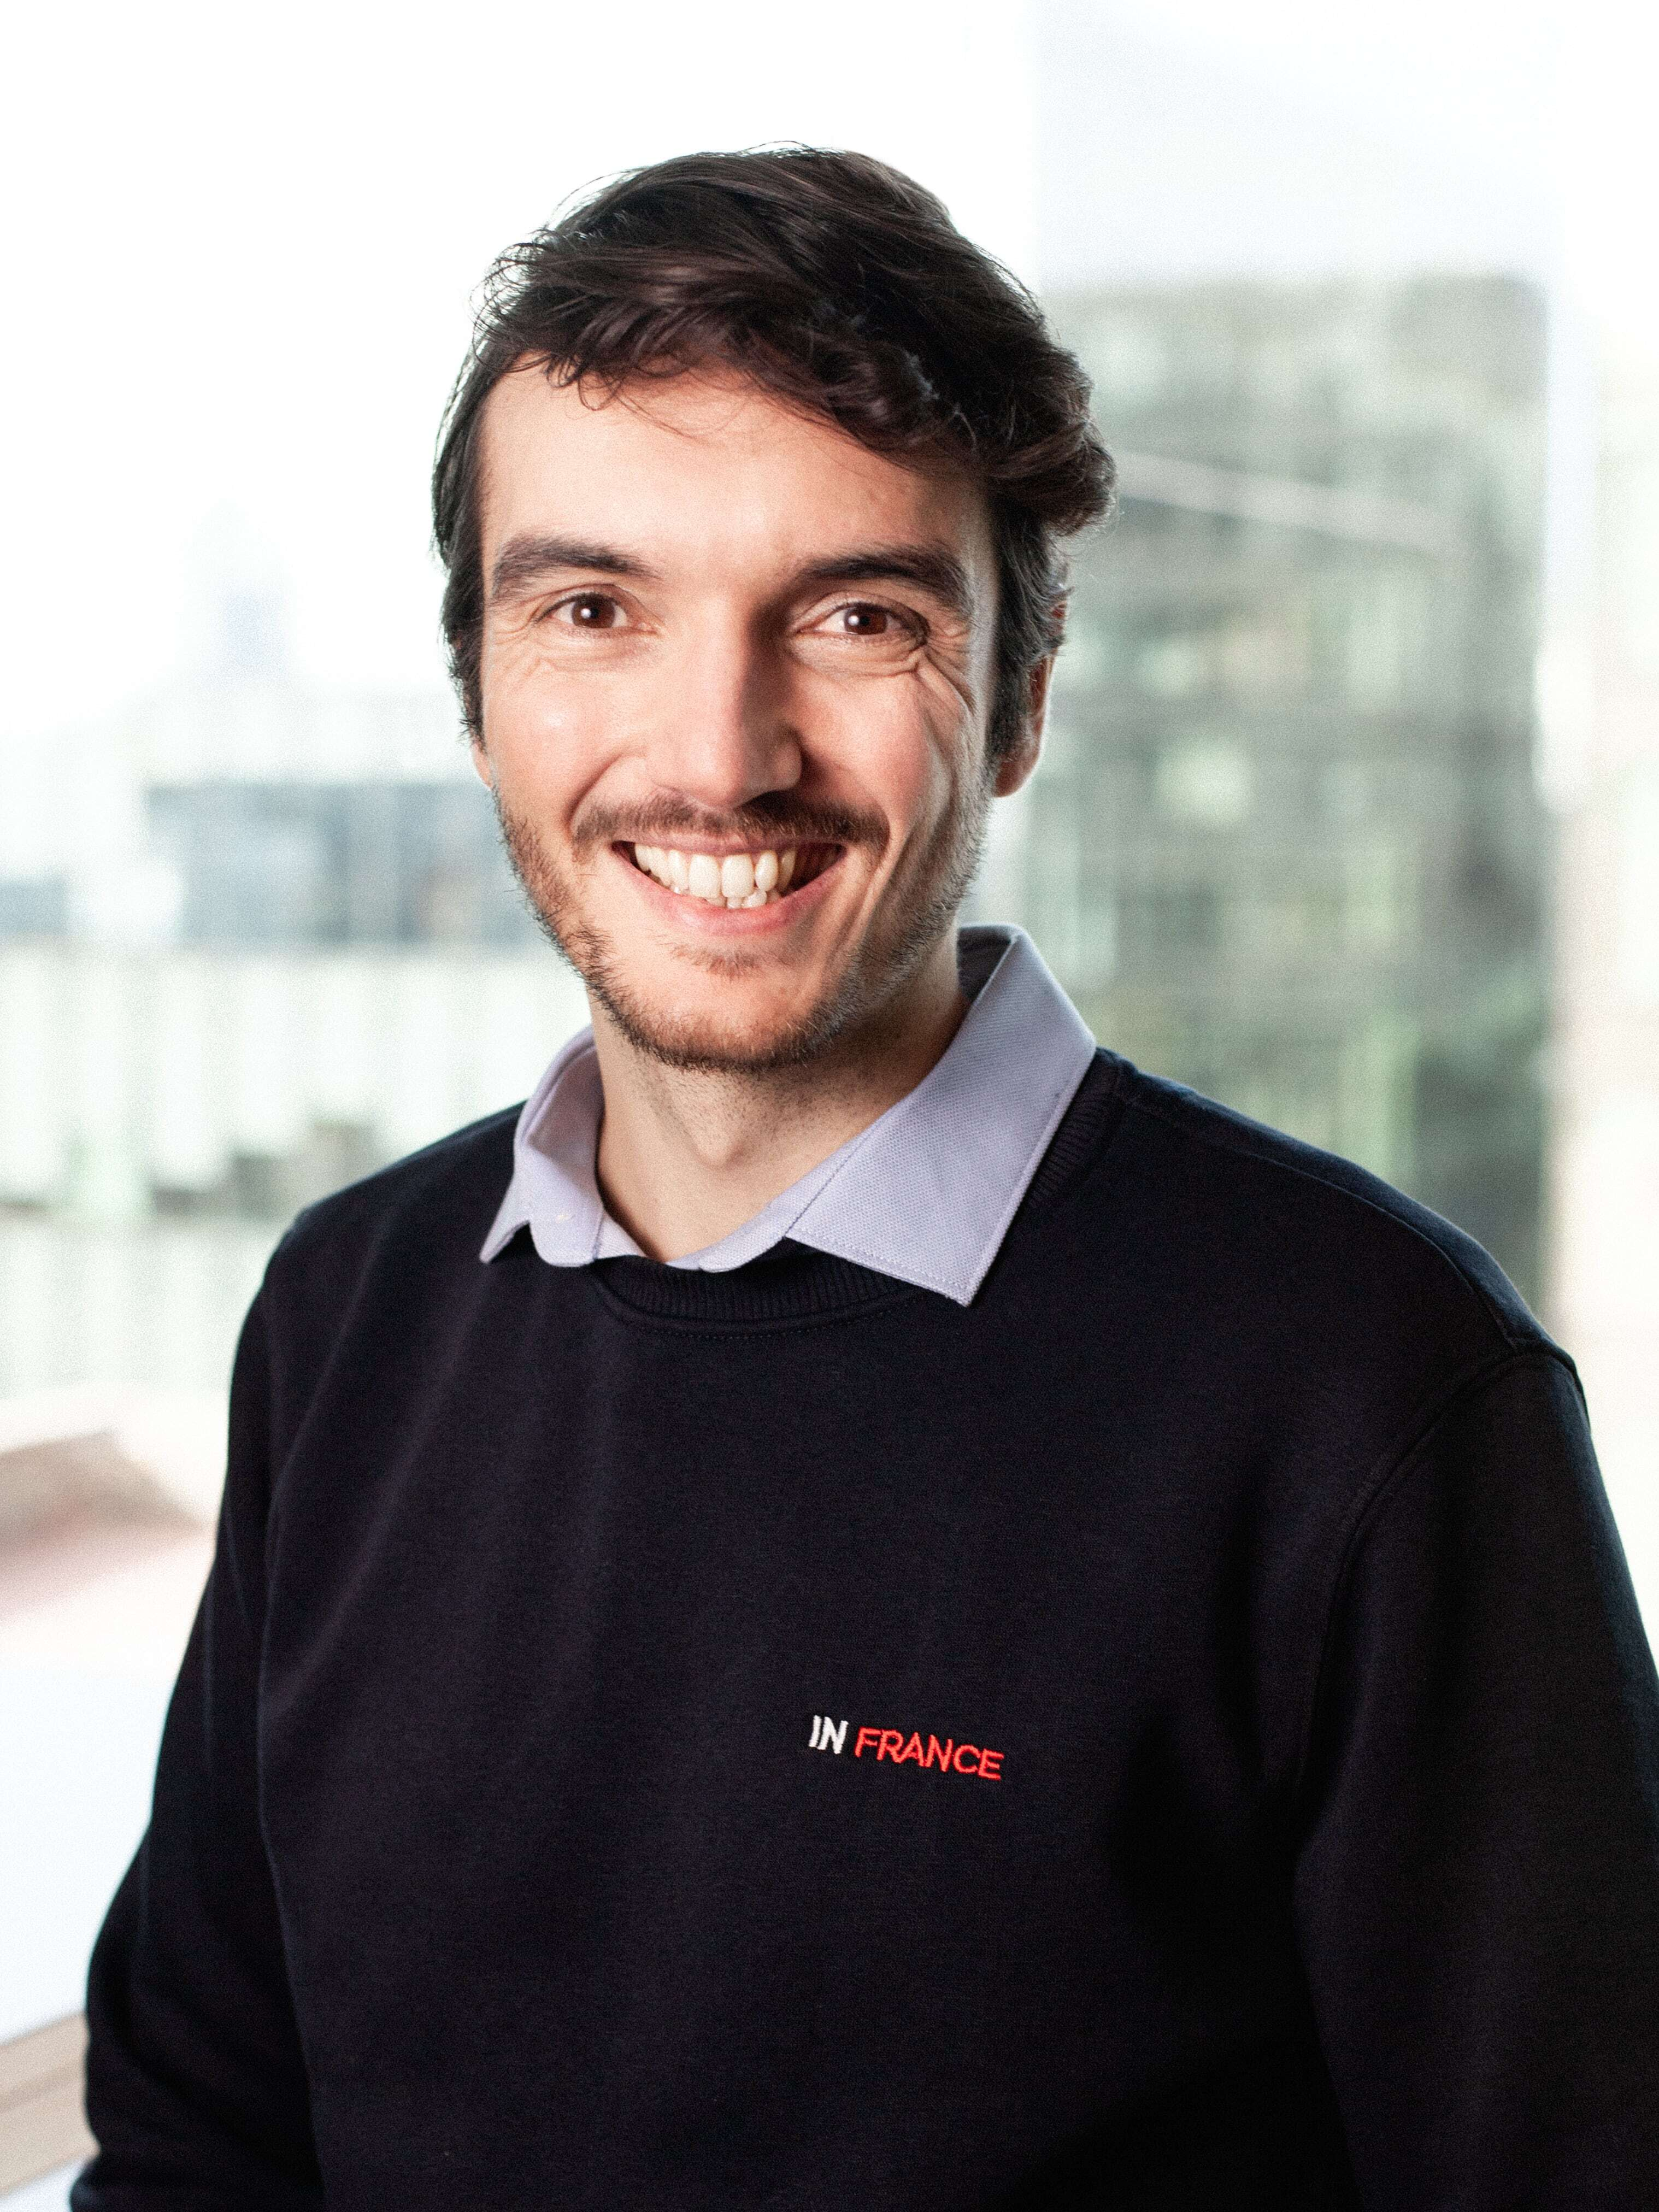
\includegraphics[width=5cm]{image/trombine-christophe}
        \end{columns}
    \end{frame}

    \subsection{Historique}\label{subsec:historique}

    \begin{frame}{Historique de Linux}{Linux, quelques caractéristiques de la première version\footnote{The early days of Linux, Lars Wirzenius, \url{https://lwn.net/Articles/928581/}}}
        \begin{footnotesize}
            \begin{itemize}
                \item La première version libérée par Linus Torvald, date de 1991 et sa licence ne permet pas l'usage commercial.
                \item Elle est compilée avec GCC 1.4, A.K.A. \textit{GNU C Compiler} de Richard Stallman.
                La publication de GCC en version 0.9 date de 1987.
                L.~Torvald a déjà porté GCC sous Minix, un OS éducatif\footnote{GCC,\url{https://gunkies.org/wiki/Gcc}}\footnotestep\footnote{A Brief Historu of GCC, \url{https://gcc.gnu.org/wiki/History}}.
                \item 1992, Linux est distribué sous license GNU GPL, donc pour tout usage, même commercial.
                \item 1992, intégration de X11, le serveur graphique, pour favoriser l'usage en \textit{desktop}.
                \item 1993, formation de la communauté Debian.
                \item Fin des années 90, les investissements d'IBM pour supporter Linux atteignent le milliard de dollars\footnote{A strong history and commitment to open source, \url{https://www.ibm.com/opensource/story/}}.
            \end{itemize}
        \end{footnotesize}
    \end{frame}

    \begin{frame}{Historique de Linux}{Historique de tous les OS\footnote{chococigar, \url{https://github.com/chococigar/cup-of-cs/blob/main/img/history\_of\_os.png}}}
        \centering
        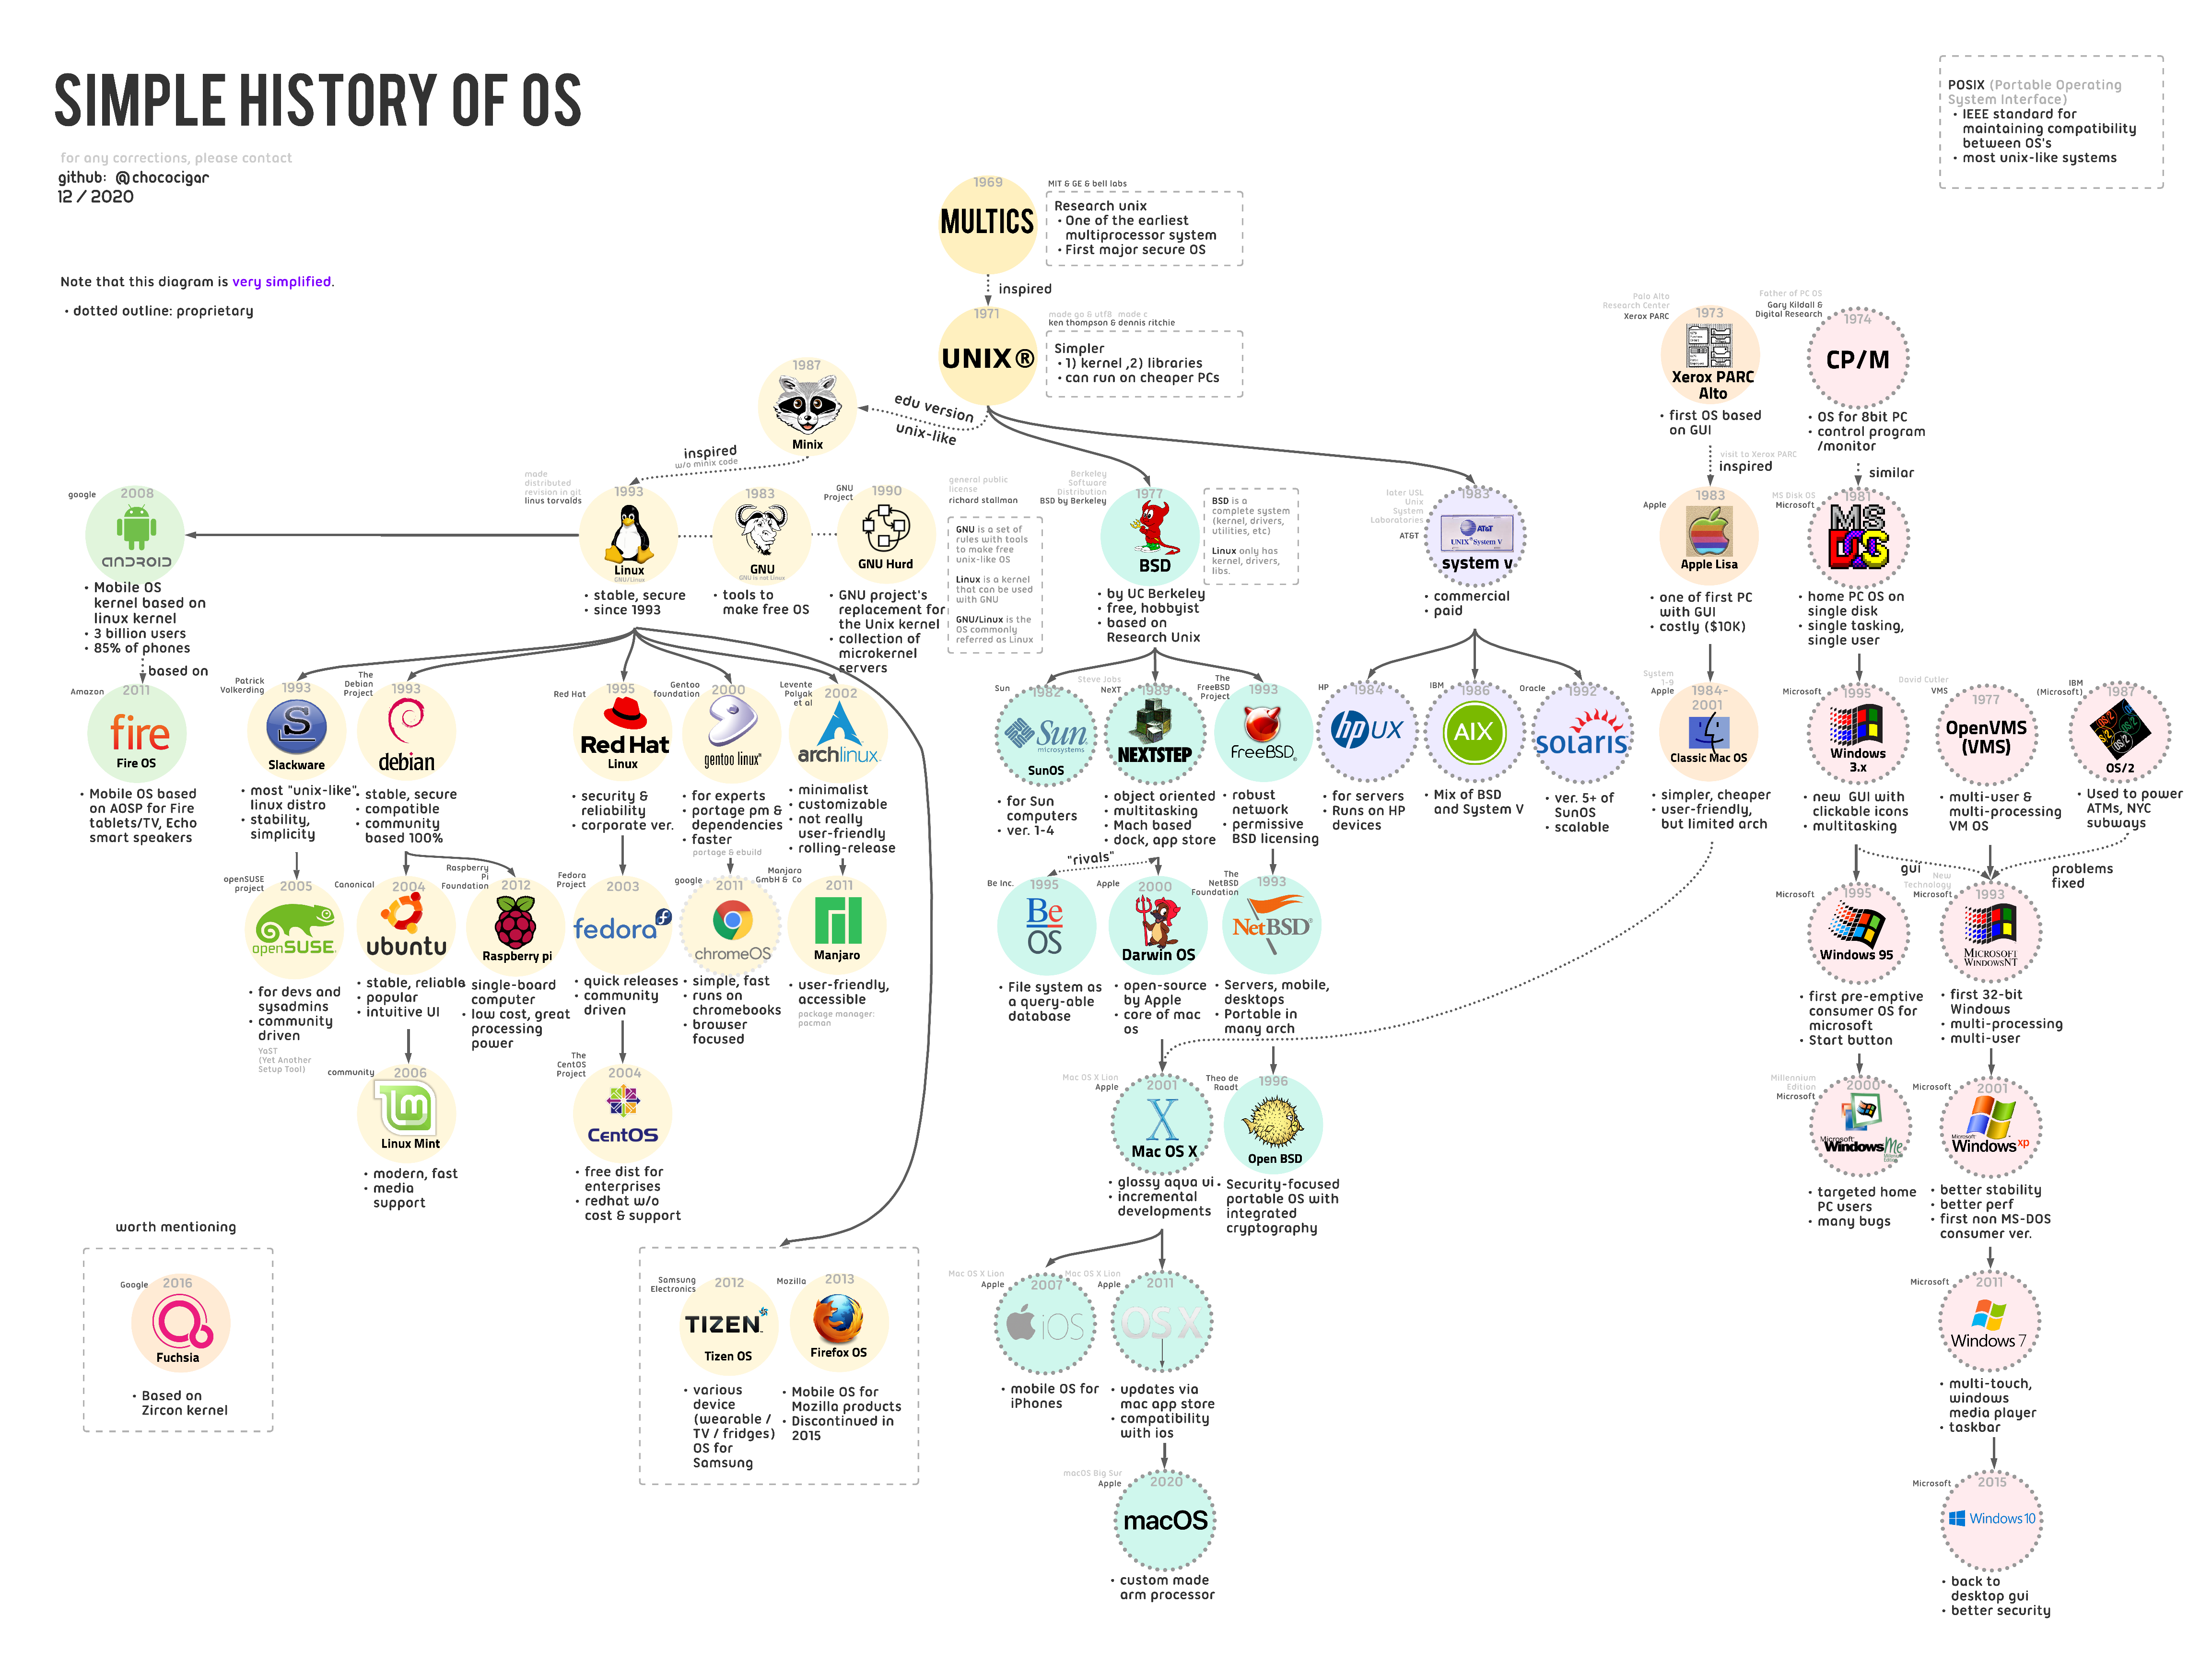
\includegraphics[width=9cm]{image/history_of_os}
    \end{frame}

    \begin{frame}{Historique de Linux}{Linux, historique des single/multi users OS}
        Multi user au sens \textit{Time-Sharing}, \textit{i.e.}, plus d'un utilisateur en même temps.

        Les premiers OS Multi user était OS/360 d'IBM dans les années 60.
        Un concurrent est développé par Bell Labs, une filiale d'AT\&T (Avant le démantèlement en 1982), c'est Unix en 1969.

        Linux est ainsi multi user dès le début.
        Par opposition à Windows, qui par défaut (sans RDP ni bricolage), ne l'est pas.
        C'est Windows® Server qui est multi user.
        \bigbreak
        Cette différence est cruciale, car elle a fait de cet OS un candidat idéal pour les serveurs (Web, BDD, \textit{etc}).
    \end{frame}

    \begin{frame}{Historique de Linux}{Adoption}
        \footnotetext{Why Linux runs 90 percent of the public cloud workload, \url{https://www.cbtnuggets.com/blog/certifications/open-source/why-linux-runs-90-percent-of-the-public-cloud-workload}}
        \footnotetext{\label{cbt}When everything is in the cloud, does the OS matter?, \url{https://www.redhat.com/en/blog/when-everything-cloud-does-os-matter}}
        \footnotetext{20 great years of Linux and supercomputer, \url{https://www.zdnet.com/article/20-great-years-of-linux-and-supercomputers/?ref=itsfoss.com}}
        \begin{columns}
            \column{0.5\textwidth}
            \begin{itemize}
                \item 2018, 90 \% des serveurs du cloud tournent sous Linux\footnotemark.
                \item 2018, 70 \% des serveurs sont déployés dans le cloud\footnotemark.
                \item 2018, 62 \% de l'embarqué\cref{cbt}.
                \item 2012, 95 \% des supercalculateurs\footnotemark.
            \end{itemize}
            \column{0.5\textwidth}
            \centering
            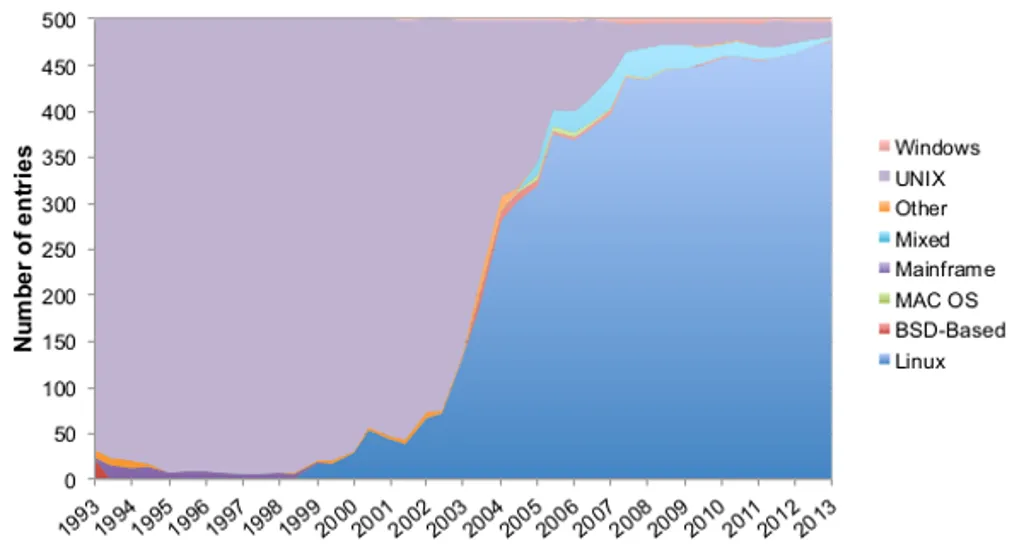
\includegraphics[width=6cm]{image/linux-supercomputer-growth}
        \end{columns}
    \end{frame}

    \subsection{Kernel et distribution}\label{subsec:kernel-et-distribution}

    \begin{frame}{Les distributions}{Définitions\footnote{Glossary, \url{https://help.ubuntu.com/community/Glossary}}}
        \begin{itemize}
            \item \textbf{Kernel} ou \textbf{Noyau}~: Le composant central d'un système d'exploitation qui contrôle tous les processus bas niveau d'un ordinateur, tels que la gestion de la mémoire, les threads et les entrées/sorties.
            En un sens, le noyau agit comme le gardien de l'ordinateur vis-à-vis du matériel.
            Les applications font des appels système via le noyau pour demander des ressources et interagir avec le matériel.
            \item \textbf{Distribution}~: Désigne une version de GNU/Linux ou d'un autre système d'exploitation open source, bien que certaines personnes soutiennent que le terme devrait inclure les différents systèmes d'exploitation Windows® et Apple.
            Ubuntu est la version la plus populaire, mais il en existe de nombreuses autres, telles que RedHat, qui est bien connue pour les serveurs.
            La plupart des autres distributions sont conçues pour un type particulier d'architecture, comme les téléphones, les netbooks, les routeurs, les serveurs, \textit{etc}.
        \end{itemize}
    \end{frame}

    \begin{frame}{Kernel}{Définition\footnote{Linux fundamentals: user space, kernel space, and the syscalls API surface, \url{https://www.form3.tech/blog/engineering/linux-fundamentals-user-kernel-space}}}
        \centering
        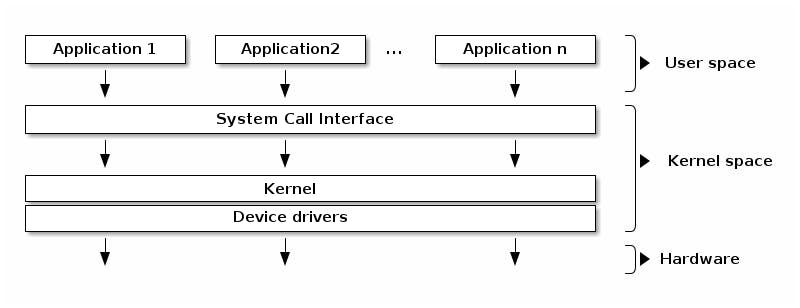
\includegraphics[width=10cm]{image/kernel}
        \flushleft
        \begin{itemize}
            \item \textbf{User space}~: L'espace utilisateur est l'endroit où les applications s'exécutent.
            \item \textbf{Kernel space}~: L'espace noyau est l'endroit où le noyau s'exécute.
            \item \textbf{Syscalls}~: Les appels système sont des interfaces entre les applications et le noyau.
        \end{itemize}
    \end{frame}

    \begin{frame}{Les distributions}{La timeline de toutes les distributions\footnote{FabioLolix, \url{https://github.com/FabioLolix/linuxtimeline}}\footnotestep\footnote{Put the fun back into computing. Use Linux, BSD., \url{https://distributionwatch.com/}}}
        \begin{columns}
            \column{0.8\textwidth}
            Insights~:
            \begin{itemize}
                \item Les 3 plus grosses branches sont Debian, Red Hat et Ubuntu.
                \item Très nombreuses.
                \item Certaines branches meurent même après de longues années d'existence (Mandrake, Centos, \textit{etc}.).
                \item Certaines distributions passent d'une branche à l'autre.
            \end{itemize}
            Quid de l'impact sur la maintenance de la distribution~?
            \column{0.2\textwidth}
            \centering
            \includegraphics[width=1.5cm]{image/linux-all-distro-timeline}
        \end{columns}
    \end{frame}

    \begin{frame}{Les distributions}{La timeline de toutes les distributions}
        Red-Hat, filiale d'IBM, fait l'opposition entre les distributions \textit{entreprise} et les \textit{community}.
        En mettant en avant leur support de 10 ans contre 2 ans pour Fedora, une distribution communautaire de la même branche\footnote{What's the best Linux distribution for you?, \url{https://www.redhat.com/en/topics/linux/whats-the-best-linux-distribution-for-you}}.
        \bigbreak
        Ubuntu a un business model légèrement différent, ils proposent 5 ans de support pour les versions LTS et une extension de 10 ans dans la version payant appelée \textquote{Ubuntu Pro}\footnote{The Ubuntu lifecycle and release cadence, \url{https://ubuntu.com/about/release-cycle}}.
        \bigbreak
        Mais peut-être que l'exemple de Red-Hat n'est pas le bon, Debian, une distribution communautaire également, communique un support des versions LTS de 5 ans minimum\footnote{Debian Long Term Support, \url{https://wiki.debian.org/LTS}}\ldots
    \end{frame}

    \begin{frame}{Les distributions}{La timeline des principales distributions\footnote{\label{main-distribution}Philipp Leclercq, \url{https://github.com/PhilLecl/SanitizedLinuxTimeline}}}
        \centering
        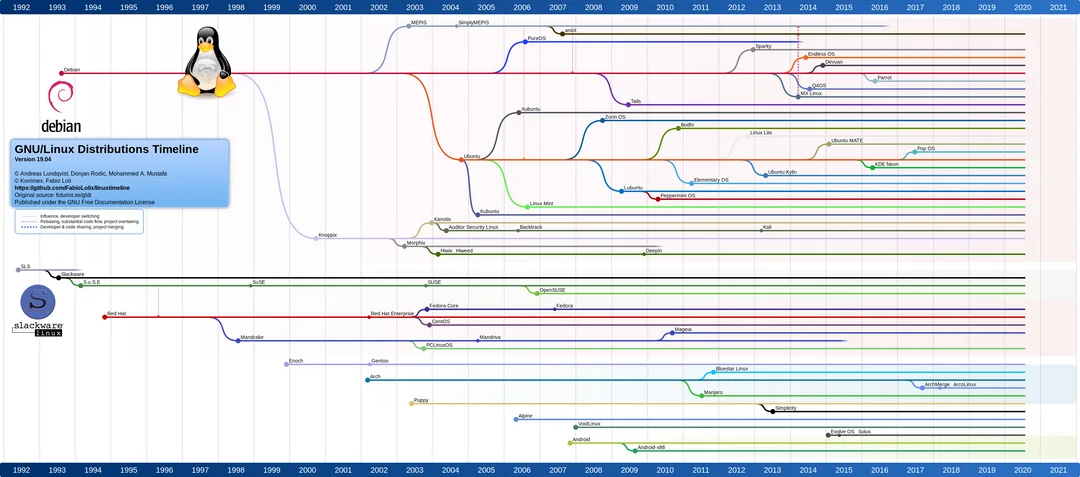
\includegraphics[width=12cm]{image/linux-main-distro-timeline}
    \end{frame}

    \begin{frame}{Les distributions}{Les licences des principales distributions\cref{main-distribution}}
        \centering
        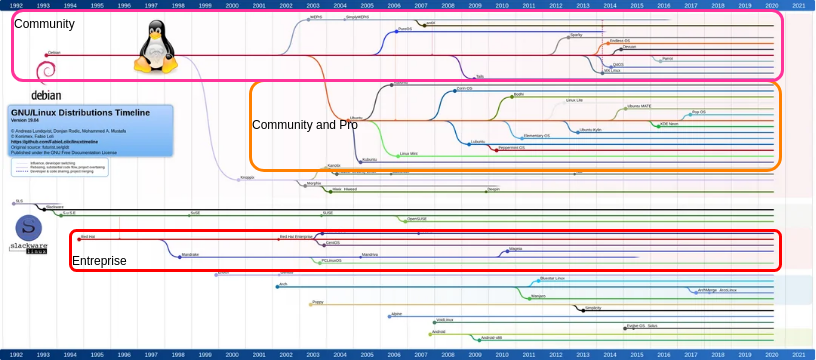
\includegraphics[width=12cm]{image/main-distro-license.drawio}
    \end{frame}

    \begin{frame}{Les distributions}{Les packages managers des principales distributions\cref{main-distribution}}
        \centering
        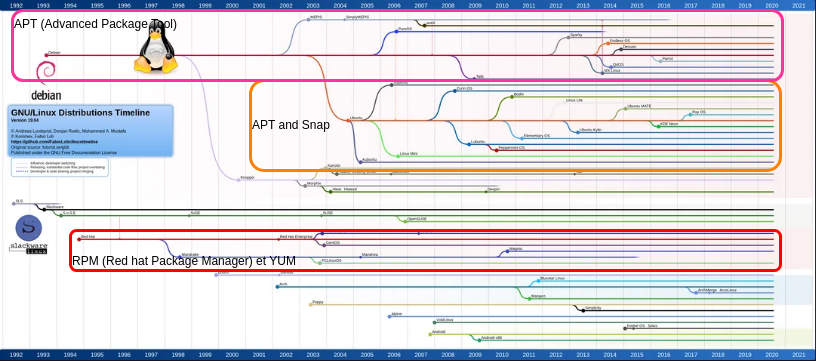
\includegraphics[width=12cm]{image/main-distro-package-manager.drawio}
    \end{frame}

    \begin{frame}{Les distributions}{Une aide pour choisir sa distribution}
        Le site Distrowatch propose un utilitaire pour trouver des distributions candidates en fonction d'un large nombre de critères, \url{https://distrowatch.com/search.php}.
        \bigbreak
        \centering
        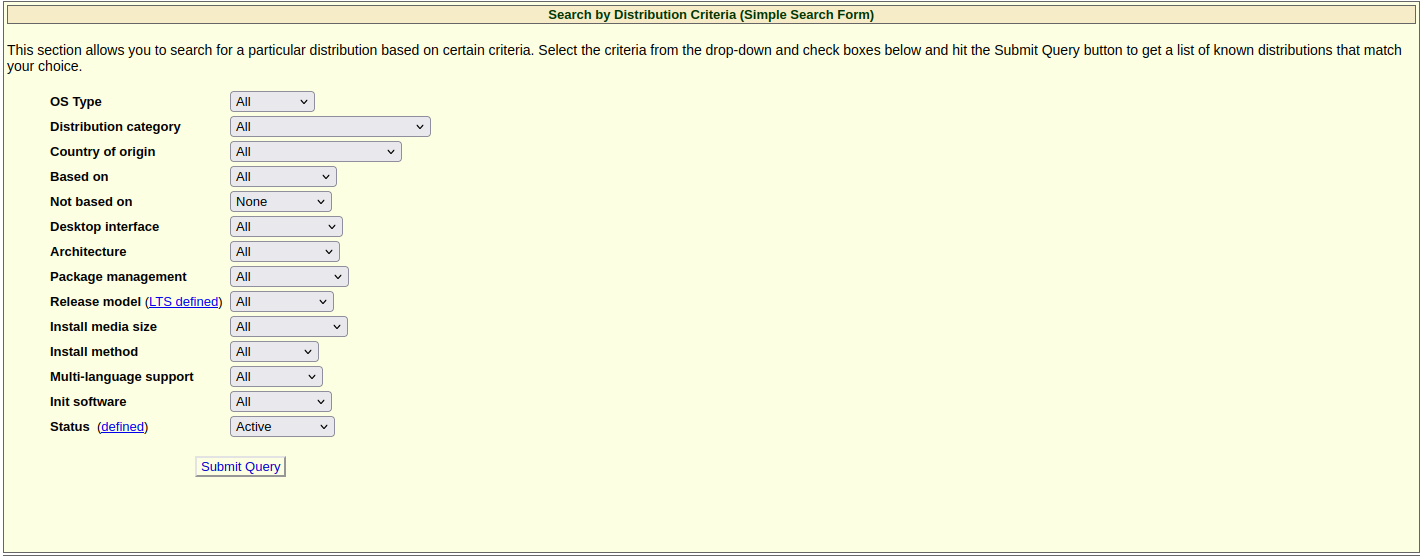
\includegraphics[width=12cm]{image/distrowatch-search}
    \end{frame}

    \begin{frame}{Les distributions}{Une aide pour choisir sa distribution}
        Admettons que tous les 2/3 packages managers mainstreams se valent.
        \bigbreak
        Un des critères différenciant, en plus du support que nous avons vu, est l'architecture.
        \bigbreak
        Qu'est-ce que le critère \textquote{architecture} et pourquoi est-ce important lors d'une migration~?
        \pause
        \bigbreak
        \begin{itemize}
            \item Une modernisation d'un hardware vieillissant qui peut être remplacé par une machine virtuelle faisant tourner les mêmes applications.
            \item Un hardware qui n'est plus supporté par la distribution actuelle et doit donc migrer.
        \end{itemize}
        Dans les 2 exemples, avoir une même architecture permettra ainsi une migration plus \textit{lean}.
        Sans rewrite, voire, sans recompilation.
    \end{frame}

    \begin{frame}{Les distributions}{Des critères manquants~?}
        Y-a-t-il des critères pertinents qui pourraient manquer~?
        \bigbreak
        \centering
        
\includegraphics[width=3cm]{image/question-mark}
    \end{frame}

    \begin{frame}{Les distributions}{Des critères manquants~?}
        L'énorme succès d'une distribution à part, Alpine Linux, pousser par les technologies de virtualisation et de conteneurisation.
        \bigbreak
        Une des premières phrases de présentation sur leur site est \textit{Alpine Linux is built around musl libc and busybox. A container requires no more than 8 MB and a minimal installation to disk requires around 130 MB of storage.}\footnote{About, \url{https://alpinelinux.org/about/}}.
        \bigbreak
        De leur analyse, qui est sûrement la bonne, leur succès vient du compilateur musl et de la librairie C libc musl.
    \end{frame}

    \begin{frame}{Les distributions}{Des critères manquants~?}
        Red-Hat recrute beaucoup d'experts de LLVM ces dernières années\footnote{Red Hat Is Hiring More LLVM Compiler Engineers, \url{https://www.phoronix.com/news/Red-Hat-More-LLVM-Engineers}}.

        Certaines distributions peuvent ou sont compilées avec LLVM comme FreeBSD\footnote{Building FreeBSD with clang/llvm, \url{https://wiki.freebsd.org/BuildingFreeBSDWithClang}}, Chimera\footnote{About Chimera Linux, \url{https://chimera-linux.org/about/}}, OpenMandriva\footnote{La communauté OpenMandriva annonce la disponibilité d'OpenMandriva Lx 4.0, \url{https://linux.developpez.com/actu/266344/La-communaute-OpenMandriva-annonce-la-disponibilite-d-OpenMandriva-Lx-4-0-qui-apporte-de-nombreuses-nouveautes-liees-a-LLVM-Clang/}}\ldots
    \end{frame}

    \begin{frame}{Les distributions}{Plusieurs combinaisons de compilateurs et libraries C}
        \centering
        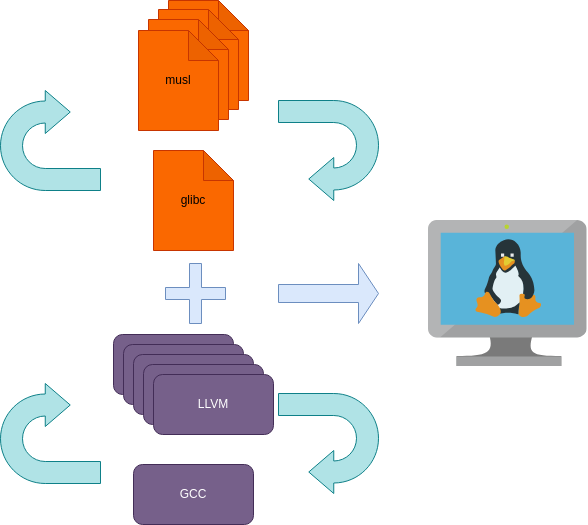
\includegraphics[width=8cm]{image/interchange-lib-compiler.drawio}
    \end{frame}

    \begin{frame}{Les distributions}{Conclusion}
        \begin{columns}
            \column{0.6\textwidth}
            Une distribution Linux est construite de manière modulaire~:
            \begin{itemize}
                \item Version de noyau.
                \item Packages manager.
                \item Architecture.
                \item Licence.
                \item Support.
                \item Librairie C~.
                \item Compilateur.
                \item \textit{Many more}.
            \end{itemize}
            \column{0.4\textwidth}
            \centering
            
\includegraphics[width=5.5cm]{image/craftsman-focused}
        \end{columns}
        \bigbreak
        À vous de trouver la meilleure combinaison pour vos besoins.
    \end{frame}


    \section{Shell et commandes de base}\label{sec:shell-and-command}

    \subsection{Shell}\label{subsec:shell}

    \begin{frame}{Shell}{Qu'est-ce~?}
        Shell c'est~:
        \begin{itemize}
            \item C'est un exécutable.
            \item Un interpréteur de ligne de commande.
            Ne pas confondre avec des Shell spécifique comme le Python Shell ou le MySQL Shell qui interagissent spécifiquement avec ces applications.
            \item Et donc un interpréteur de scripts Shell.
            \item C'est une interface entre l'OS et l'humain.
            \item Existe sur la plupart des plateformes Linux, Unix, Windows® (\lstinline{Bash}, installé avec Git par exemple), \textit{etc}.
            \item Une portabilité poussée par une standardisation, comme la standardisation POSIX~.
            \item Des Shells plus \textit{user friendly} et plus lourds comme \lstinline{zsh}.
            \item Des Shells éxotiques comme \lstinline{tcsh} et \lstinline{csh}.
        \end{itemize}
    \end{frame}

    \begin{frame}{Shell}{Bourne Shell VS Bourne Again Shell\footnote{Difference between sh and bash, \url{https://www.geeksforgeeks.org/difference-between-sh-and-bash/}}}
        \begin{footnotesize}
            \begin{table}[h!]
                \centering
                \begin{tabular}{|p{5.5cm}|p{5.5cm}|}
                    \hline
                    \textbf{bash}                                     & \textbf{sh}                               \\ \hline
                    Bourne Again SHell                                & SHell                                     \\ \hline
                    Developed by Brain Fox                            & Developed by Stephen R. Bourne            \\ \hline
                    Successor of sh                                   & Predecessor of bash                       \\ \hline
                    bash is the default SHELL                         & sh is not the default SHELL               \\ \hline
                    \lstinline{\#\!/bin/bash}                         & \lstinline{\#\!/bin/sh}                   \\ \hline
                    It has more functionality with up-gradation       & It has less functionality                 \\ \hline
                    Supports job controls                             & Does not support job control              \\ \hline
                    bash is not a valid POSIX shell                   & sh is a valid POSIX shell                 \\ \hline
                    Easy to use                                       & Not as easy as bash                       \\ \hline
                    Less portable than sh                             & More portable than bash                   \\ \hline
                    Extended version of language                      & Original language                         \\ \hline
                    Bash scripting is scripting specifically for Bash & Shell scripting is scripting in any shell \\ \hline
                    Supports command history                          & Does not support command history          \\ \hline
                \end{tabular}
            \end{table}
        \end{footnotesize}
    \end{frame}

    \begin{frame}[fragile]{Shell}{Qu'est-ce~?}
        2 Shells sous une même distribution \textquote{légère} comme Alpine Linux~:
        \begin{lstlisting}[language=bash]
root@71641013d445:/usr/src/celia# sh
# ls
 Dockerfile       README.pdf         UML-Sequence.drawio       celia.ipynb
# which sh
/usr/bin/sh
# which ls
/usr/bin/ls
# bash
root@71641013d445:/usr/src/celia# which bash
/usr/bin/bash
root@71641013d445:/usr/src/celia# which ls
/usr/bin/ls
root@71641013d445:/usr/src/celia# ls
 Dockerfile       README.pdf         UML-Sequence.drawio       celia.ipynb
        \end{lstlisting}
        \bigbreak
        Comment interpréter ce code~?
    \end{frame}

    \begin{frame}{Shell}{Qu'est-ce~?}
        \begin{itemize}
            \item Un interpréteur de lignes de commandes.
            \item \lstinline{sh} et \lstinline{bash} peuvent appeler les mêmes exécutables.
            \item \lstinline{sh} et \lstinline{bash} n'ont pas des scripts compatibles.
            \item \lstinline{sh}, le Shell POSIX ou Bourne Shell est plus léger et plus rapide que \lstinline{bash}.
            \item \lstinline{bash}, le Bourne Again Shell est plus complet et plus facile à utiliser.
            \item Shell n'est qu'une interface.
            \item Même dans une distribution \textquote{lightweight}, il y a 2 interpréteurs Shell~!
        \end{itemize}
        \begin{columns}
            \column{0.7\textwidth}
            \lstinline{bash}, n'est pas installé par défault sur la dernière version de FreeBSD 14, uniquement \lstinline{sh}.
            Qu'en penser~?
            \column{0.3\textwidth}
            \centering
            
\includegraphics[width=3cm]{image/guy-in-front-of-desktop}
        \end{columns}
    \end{frame}

    \begin{frame}{Shell}{Bourne Shell VS Bourne Again Shell}
        Peut-on lister les avantages/inconvénients de l'un et l'autre~?
        \bigbreak
        \centering
        
\includegraphics[width=3cm]{image/question-mark}
    \end{frame}

    \begin{frame}{Shell}{Le poid de cette interface\footnote{Exigences matérielles pour utiliser Ubuntu, \url{https://doc.ubuntu-fr.org/exigences_minimales}}}
        Minimum 30 Go d'espace disque disponible pour une installation avec GNOME contre 5 Go ou 6 Go pour une installation Server ou Cloud.
        \bigbreak
        L'absence de bureau, avoir uniquement cette interface, est une des raisons de cette différence de taille.

        L'interface graphique n'est donc pas installé dans les distributions dédiées aux serveurs.
        Shell et l'accès Shell distant sécurisé \lstinline{SSH} (Secure SHell), sont utilisés.
        Un client SSH comme Putty, SSH de GitBASH sous Windows® ou un terminal sous Linux permettent d'accéder à un server Linux.
        \bigbreak
        GitBash permet d'unifier les deux environnements Linux et Windows, de pratiquer le Bash sur les 2 plateformes.
    \end{frame}

    \begin{frame}{Shell}{Pourquoi a-t-on un Shell ou l'autre~?}
        Quand je me connecte avec mon utilisateur, j'ai souvent \lstinline{bash} comme Shell.
        Pourquoi pas \lstinline{sh}~?
        \bigbreak
        \centering
        
\includegraphics[width=3cm]{image/question-mark}
    \end{frame}

    \begin{frame}[fragile]{Shell}{Pourquoi a-t-on un Shell ou l'autre~?}
        Probablement, l'administrateur système a créé votre utilisateur en spécifiant \lstinline{bash} comme Shell.
        \bigbreak
        Si on lit l'aide de la commande \lstinline{useradd}~:
        \begin{lstlisting}[language=bash]
$ useradd -h | grep shell
  -s, --shell SHELL               interpréteur de commandes de connexion du nouveau compte
        \end{lstlisting}
        \bigbreak
        Un exemple de commande devient donc~:
        \begin{lstlisting}[language=bash]
$ useradd -s /bin/bash -m -d $/home/digiformateur digicomp
        \end{lstlisting}
        \bigbreak
        \lstinline{/bin/bash} passé à l'option \lstinline{-s} permet de spécifier le Shell.
    \end{frame}

    \begin{frame}{Shell}{Naviguer dans les commandes}
        \begin{itemize}
            \item \lstinline{history}~: Affiche l'historique des commandes.
            \item Ctrl+c~: Arrête l'exécution d'une commande.
            \item \emoji{up-arrow}~: Rappelle la dernière commande.
            \item \emoji{down-arrow}~: Rappelle la commande suivante.
            \item Ctrl+r~: Recherche dans l'historique des commandes.
            \item \lstinline{\\}~: Permet de continuer une commande sur la ligne d'après.
            \item \lstinline{\&}~: Lancer une commande en arrière-plan.
            \item Ctrl+z~: Mettre une commande en pause.
            \item \lstinline{fg}~: Reprendre une commande en pause.
            \item \lstinline{bg}~: Reprendre une commande en pause en arrière-plan.
        \end{itemize}
    \end{frame}

    \begin{frame}{Shell}{Gérer plusieurs commandes en parallèle avec \lstinline{tmux}\footnote{\label{tmux}Tmux (terminal multiplexer), \url{https://www.redhat.com/sysadmin/introduction-tmux-linux}}}
        \lstinline{tmux} est un multiplexeur de terminal, \textit{i.e.}, permet d'ouvrir plusieurs fenêtres dans un terminal.
        Chacune faisant tourner un processus.
        \begin{footnotesize}
            \begin{table}[ht]
                \centering
                \begin{tabular}{|p{3.5cm}|p{8cm}|}
                    \hline
                    \textbf{Commande}         & \textbf{Description}                                                            \\
                    \hline
                    Ctrl+b puis D             & Détacher de la session courante                                                 \\
                    \hline
                    Ctrl+b puis \%            & Diviser la fenêtre en deux volets horizontalement                               \\
                    \hline
                    Ctrl+b puis ``            & Diviser la fenêtre en deux volets verticalement                                 \\
                    \hline
                    Ctrl+b puis Flèche        & Se déplacer entre les volets                                                    \\
                    \hline
                    Ctrl+b puis X             & Fermer le volet                                                                 \\
                    \hline
                    Ctrl+b puis C             & Créer une nouvelle fenêtre                                                      \\
                    \hline
                    Ctrl+b puis N ou P        & Passer à la fenêtre suivante ou précédente                                      \\
                    \hline
                    Ctrl+b puis 0 (1,2\ldots) & Aller à une fenêtre spécifique par numéro                                       \\
                    \hline
                    Ctrl+b puis~:             & Entrer dans la ligne de commande pour taper des commandes (avec autocomplétion) \\
                    \hline
                    Ctrl+b puis ?             & Voir tous les raccourcis clavier (appuyer sur Q pour quitter)                   \\
                    \hline
                    Ctrl+b puis W             & Ouvrir un panneau pour naviguer entre les fenêtres de plusieurs sessions        \\
                    \hline
                \end{tabular}
            \end{table}
        \end{footnotesize}
    \end{frame}

    \begin{frame}{Shell}{Gérer plusieurs commandes en parallèle avec \lstinline{tmux}\cref{tmux}}
        Par exemple pour monitorer les ressources avec \lstinline{top} dans le terminal de droite, pendant qu'on lance la commande dans celui de gauche.
        \bigbreak
        \centering
        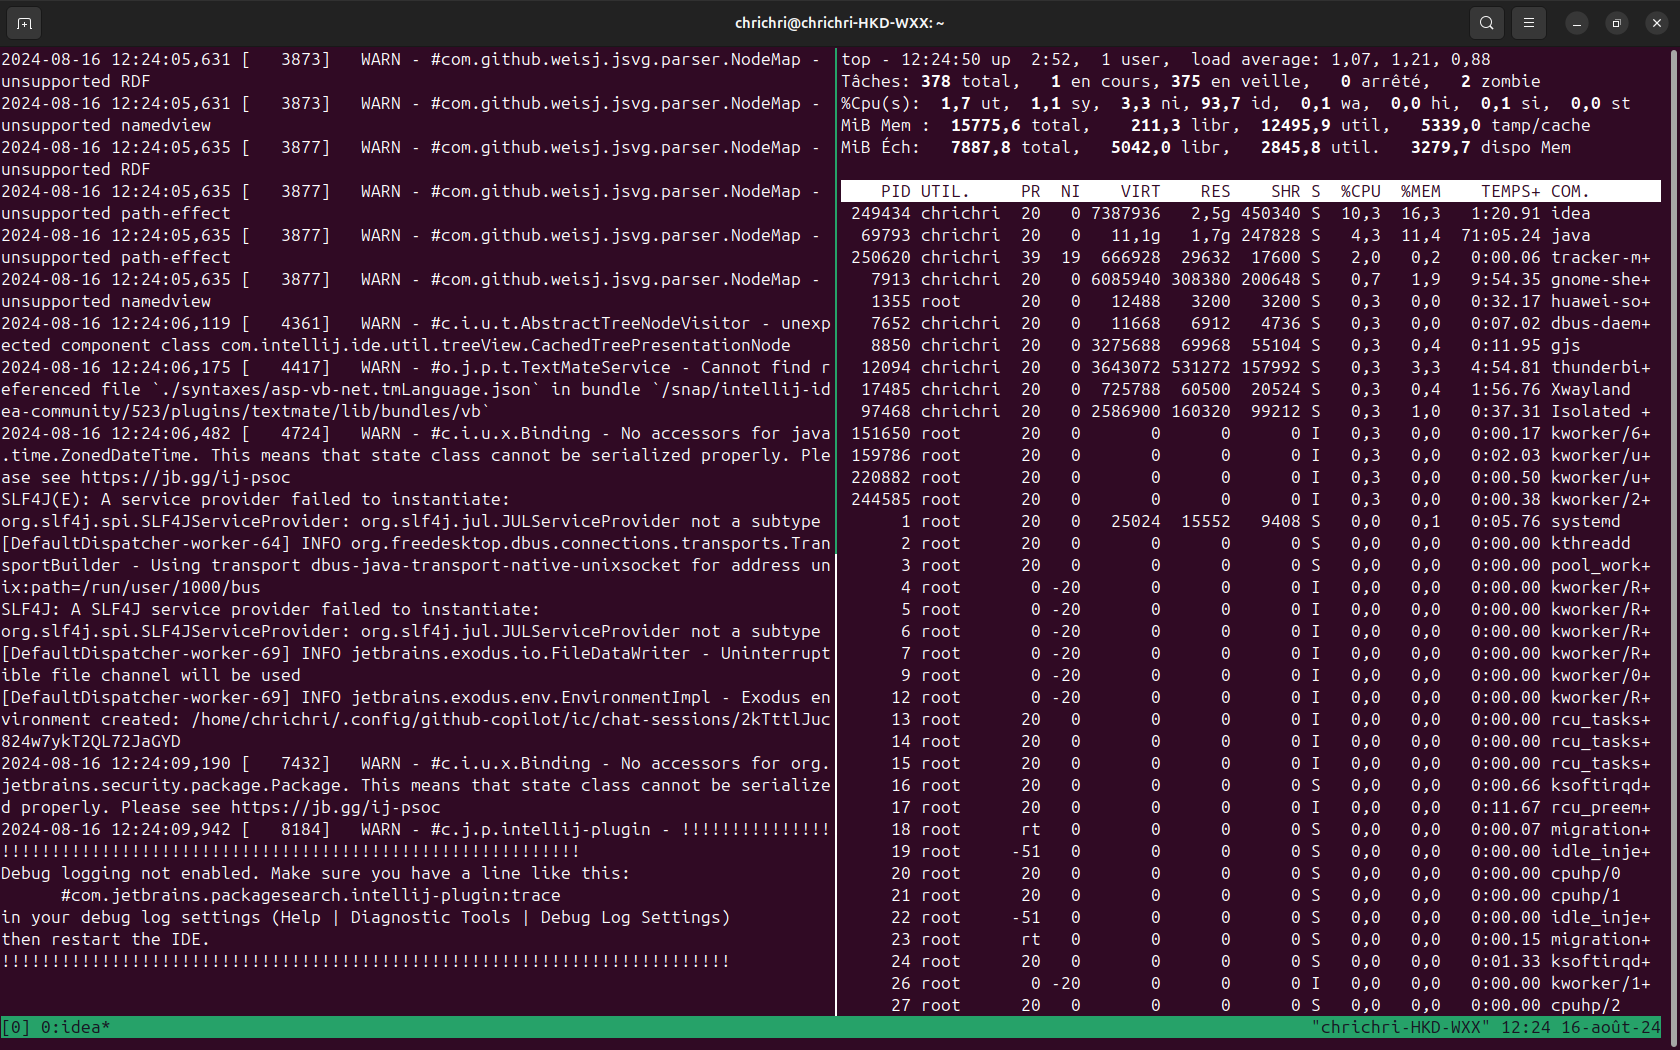
\includegraphics[width=10.3cm]{image/tmux-illustration}
    \end{frame}

    \begin{frame}[fragile]{Shell}{Gérer plusieurs commandes en parallèle avec \lstinline{nohup}}
        \lstinline{nohup} vient de NO Hang UP, c'est une commande qui permet de lancer une autre commande en arrière-plan sans qu'elle soit interrompue par la fermeture de la session Shell.
        Idéale donc pour les longs processus.
        L'output de la commande va par défault dans le fichier \lstinline{nohup.out}.
        \bigbreak
        Il suffit de préfixer la commande par \lstinline{nohup} et d'ajouter un \lstinline{&} pour libérer le terminal.
        \lstinline{nohup} indique le PID pour pouvoir stopper la commande au besoin et indique également quand la commande est terminée, si elle s'est arrêtée (Termine <code retour>) prématurément ou normalement (Fini).
        \begin{lstlisting}[language=bash]
$ nohup ls &
[1] 279343
nohup: les entrées sont ignorées et la sortie est ajoutée à 'nohup.out'
[1]+  Fini                    nohup ls
$ tail -n 3 nohup.out
technip
Téléchargements
ts-test
        \end{lstlisting}
    \end{frame}

    \begin{frame}[fragile]{Shell}{Les alias}
        Les alias sont des raccourcis pour des commandes.
        ils sont donc intéressant à paramétrer pour les commandes longues et récurrente.
        \bigbreak
        Par exemple, pour la commande \lstinline{ls -l}~:
        \begin{lstlisting}[language=bash]
$ alias ll='ls -l'
$ ll
total 3484
-rw-rw-r-- 1 chrichri chrichri     249 août  15 12:35 analytic-using-awk.sh
-rw-rw-r-- 1 chrichri chrichri      82 août  10 23:04 checkmytex.sh
...
        \end{lstlisting}
        \bigbreak
        Pour rendre l'alias permanent, il faut l'ajouter dans le fichier \lstinline{.bashrc} ou \lstinline{.bash\_profile}~:
        \begin{lstlisting}[language=bash]
$ echo "alias ll='ls -l'" >> ~/.bashrc
        \end{lstlisting}
        De cette manière à chaque fois qu'un Shell est ouvert, la commande est exécutée.
    \end{frame}

    \begin{frame}{Shell}{Secure SHell (SSH)}
        La machine Linux à administrer sera le plus souvent dans un cloud, une salle serveur, un data center, elle sera distante.
        Dans une infrastructure sécurisée.
        \bigbreak
        Mais avec un user, un Shell par défaut, et un protocole sécurisé comme le SSH~.
        Nous allons pouvoir nous connecter et l'administrer à distance.
        \bigbreak
        Les bonnes pratiques sont d'utiliser les clés SSH uniquement, pas de connexion SSH avec l'utilisateur root,
        Tutoriel utile~:
        \begin{itemize}
            \item \href{https://phoenixnap.com/kb/generate-setup-ssh-key-ubuntu}{Configuration du login SSH sur Ubuntu}
        \end{itemize}
        \bigbreak
        \centering
        
\includegraphics[width=3cm]{image/guy-in-front-of-desktop}
    \end{frame}

    \begin{frame}{Shell}{Sécurisation du SSH avec la cryptographie asymétrique}
        \begin{small}
            Pourquoi est-ce plus sécure d'utiliser une clé SSH plutôt qu'un mot de passe~?
            \bigbreak
            Quels algorithmes et taille de clés sont recommandés~?
            \pause
            \bigbreak
            Sur le site \url{https://jadaptive.com/ssh-key-management/the-benefits-of-ssh-key-authentication/} on trouve~:
            \begin{columns}
                \begin{column}{0.6\textwidth}
                    \begin{itemize}
                        \item Le mot de passe doit être communiqué à chaque connexion, il est donc plus vulnérable à une interception/sniffing/MITHM~.
                        La clé privée reste sur le client, elle n'est pas communiquée.
                        \item La clé SSH est plus complexe à deviner qu'un mot de passe.
                        \item On peut automatiser des taches depuis la machine cliente avec la clé SSH~.
                    \end{itemize}
                \end{column}
                \begin{column}{0.4\textwidth}
                    \centering
                    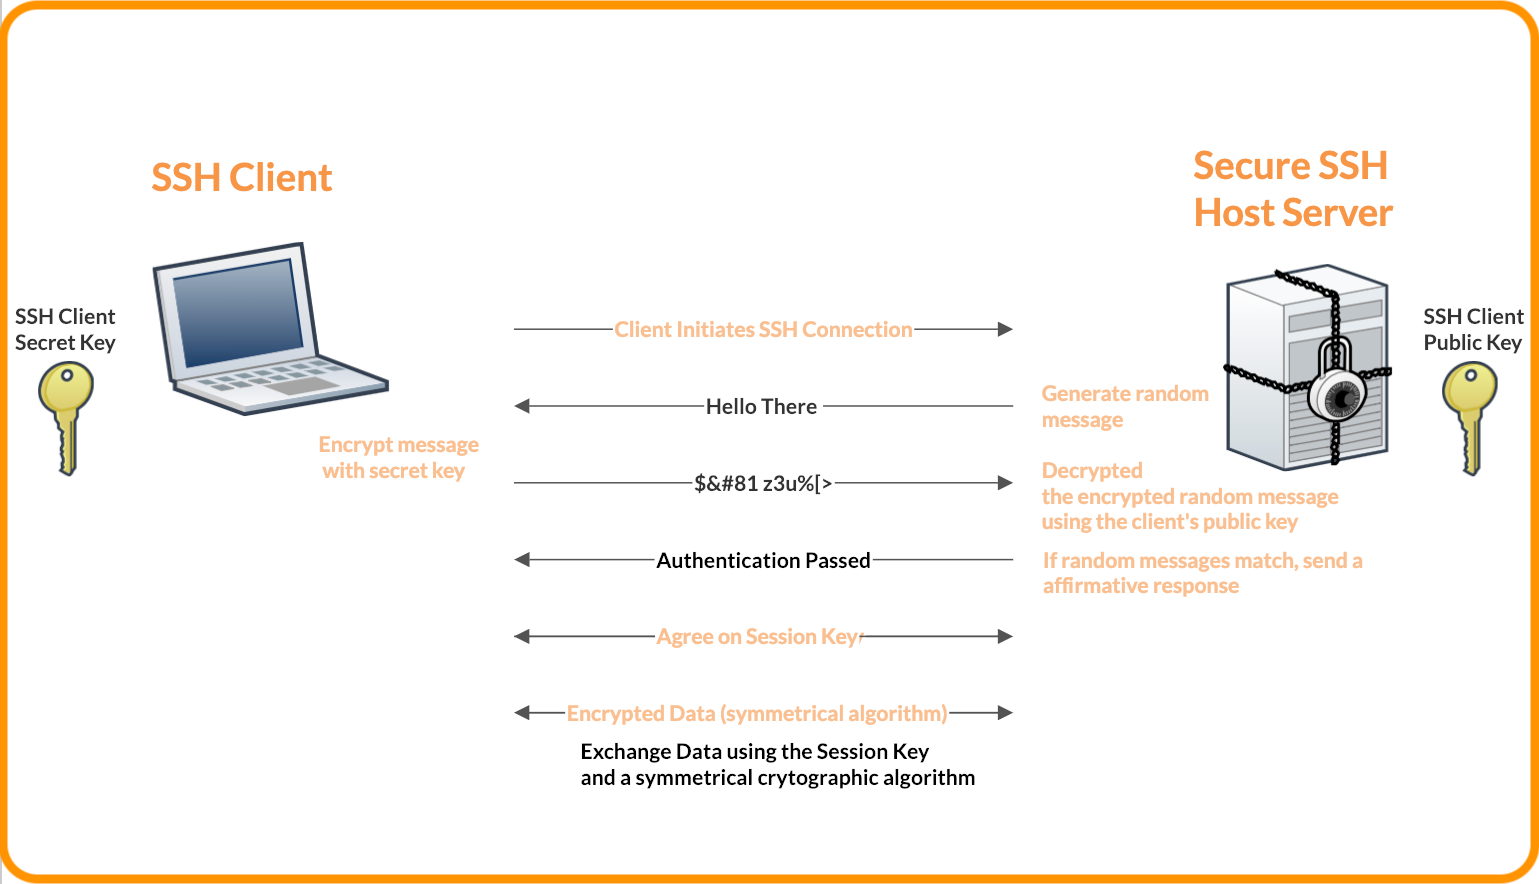
\includegraphics[width=5cm]{image/ssh-key-diagram} \\ Foxpass\footnotemark \\
                \end{column}
            \end{columns}
        \end{small}
    \end{frame}

    \begin{frame}{Shell}{Sécurisation du SSH avec la cryptographie asymétrique}
        Exercice \execcounterdispinc{}~:
        Restreindre l'accès à la VM au SSH avec une clé SSH, aucun mot de passe.
        \bigbreak
        Exercice \execcounterdispinc{}~:
        Créer un user pour un de vos camarades.
        Lui donner un Shell \lstinline{sh} par défaut.
        Configurer lui communiquer les clés SSH pour qu'il puisse se connecter.
    \end{frame}

    \begin{frame}[fragile]{Shell}{Une des solutions (commande à exécuter sur la VM)}
        Commande pour configurer la VM~:
        \begin{lstlisting}[language=bash][fragile]
# Configure SSH
$ sudo sed -i 's/PermitRootLogin yes/PermitRootLogin no/' /etc/ssh/sshd_config
$ sudo sed -i 's/PasswordAuthentication yes/PasswordAuthentication no/' /etc/ssh/sshd_config
# Restart SSH with the new configuration
$ sudo systemctl restart sshd
# Create the .ssh directory and the authorized_keys file
$ mkdir -p ~/.ssh
$ touch ~/.ssh/authorized_keys
# Add the public key to the authorized_keys file
$ echo "ssh-rsa AAAAB3NzaC1yc2EAAAADAQABAAABgQDQ8z4... chrichri@localhost" >> ~/.ssh/authorized_keys
        \end{lstlisting}
        \begin{center}
            
\includegraphics[width=2cm]{image/digicomp-lightbulb} \\ Expliquer chaque commande \\
        \end{center}
    \end{frame}

    \begin{frame}[fragile]{Shell}{Exemple de sécurisation des clés et des secrets sous Linux}
        Par défaut, Ubuntu desktop s’installe sur une partition non
        chiffrée (encrypter, ce n’est pas français on dit chiffrer~!~).
        Tout document peut donc être lu avec un disque de
        démarrage (live CD, USB bootable, \textit{etc}) ou si le disque dur
        est extrait et lu (vol, perte du desktop\ldots).
        \bigbreak
        Avec le package \lstinline{ecryptfs-utils} on peut chiffrer une partition~:
        \begin{lstlisting}[language=bash]
$ sudo apt-get install ecryptfs-utils
$ ecryptfs-setup-private
$ cp -r .ssh/ Private/ # Pour proteger les clés SSH on les déplace
$ ln -s /home/<mon user Ubuntu>/Private/.ssh/ . # Lien symbolique
        \end{lstlisting}
        Output~:
        \begin{lstlisting}
$ ls ~/.ssh -d -lha
lrwxrwxrwx 1 chrichri chrichri 28 janv. 14 21:27 /home/chrichri/.ssh -> /home/chrichri/Private/.ssh/
        \end{lstlisting}
        Il utilise le mot de passe de la session pour chiffrer/déchiffrer.
        Si la session n'est pas ouverte, les données sont chiffrées.
    \end{frame}

    \subsection{Commandes de base}\label{subsec:commandes-de-base}

    \begin{frame}{Commandes de base}{Commandes de base}
        \begin{itemize}
            \item \lstinline{ls}~: Liste les fichiers et répertoires.
            \item \lstinline{cd}~: Change de répertoire.
            \item \lstinline{pwd}~: Affiche le répertoire courant.
            \item \lstinline{cp}~: Copie des fichiers et des répertoires.
            \item \lstinline{mv}~: Déplace des fichiers et des répertoires.
            \item \lstinline{rm}~: Supprime des fichiers et des répertoires.
            \item \lstinline{mkdir}~: Crée des répertoires.
            \item \lstinline{cat}~: Affiche le contenu d'un fichier.
            \item \lstinline{head}~: Affiche les premières lignes d'un fichier.
            \item \lstinline{tail}~: Affiche les dernières lignes d'un fichier.
            \item \lstinline{touch}~: Crée un fichier vide.
            \item \lstinline{echo}~: Affiche une chaîne de caractères.
            \item \lstinline{du}~: Affiche l'espace disque utilisé par les fichiers.
            \item \lstinline{wget}~: Télécharge un fichier depuis URL~.
        \end{itemize}
    \end{frame}

    \begin{frame}[fragile]{Commandes de base}{Les options}
        Mais souvent, une commande seule ne suffit pas, il faut utiliser des options.

        Il existe deux solutions pour découvrir ces options~:
        \begin{itemize}
            \item Utiliser l'aide de la commande.
            Le plus souvent avec l'option \lstinline{-h}, équivalente à \lstinline{--help}.
            \begin{lstlisting}[language=bash]
$ ls --help # -h c'est human readable avec ls...
            \end{lstlisting}
            \item Ce qui revient à lire la documentation de la commande avec la commande~:
            \begin{lstlisting}[language=bash]
$ man ls # Same as above
            \end{lstlisting}
        \end{itemize}
    \end{frame}

    \begin{frame}[fragile]{Commandes de base}{Busy box}
        BusyBox est un logiciel libre qui fournit une implémentation unique d'environ 200 commandes UNIX standards dans un seul fichier pour diminuer la taille de ces derniers.
        Des distributions comme Alpine Linux l'utilisent pour réduire la taille de l'OS~.
        \begin{lstlisting}[language=bash,basicstyle=\tiny\ttfamily]
$ busybox
BusyBox v1.36.1 (Ubuntu 1:1.36.1-6ubuntu3) multi-call binary.
BusyBox is copyrighted by many authors between 1998-2015.
Licensed under GPLv2. See source distribution for detailed
copyright notices.

Usage: busybox [function [arguments]...]
   or: busybox --list[-full]
   or: busybox --install [-s] [DIR]
   or: function [arguments]...

        BusyBox is a multi-call binary that combines many common Unix
        utilities into a single executable.  The shell in this build
        is configured to run built-in utilities without $PATH search.
        You don't need to install a link to busybox for each utility.
        To run external program, use full path (/sbin/ip instead of ip).

Currently defined functions:
        [, [[, acpid, adjtimex, ar, arch, arp, arping, ascii, ash, awk, base64, basename, bc, blkdiscard, blockdev, brctl, bunzip2, busybox, bzcat, bzip2, cal, cat, chgrp, chmod, chown, chpasswd, chroot, chvt, clear, cmp, cp,
        cpio, crc32, crond, crontab, cttyhack, cut, date, dc, dd, deallocvt, depmod, devmem, df, diff, dirname, dmesg, dnsdomainname, dos2unix, dpkg, dpkg-deb, du, dumpkmap, dumpleases, echo, ed,
        \end{lstlisting}
    \end{frame}
    \begin{frame}[fragile]{Commandes de base}{Busy box}
        \begin{lstlisting}[language=bash,basicstyle=\tiny\ttfamily]
        egrep, env, expand, expr, factor,
        fallocate, false, fatattr, fdisk, fgrep, find, findfs, fold, free, freeramdisk, fsfreeze, fstrim, ftpget, ftpput, getopt, getty, grep, groups, gunzip, gzip, halt, head, hexdump, hostid, hostname, httpd, hwclock, i2cdetect,
        i2cdump, i2cget, i2cset, i2ctransfer, id, ifconfig, ifdown, ifup, init, insmod, ionice, ip, ipcalc, kill, killall, klogd, last, less, link, linux32, linux64, linuxrc, ln, loadfont, loadkmap, logger, login, logname,
        logread, losetup, ls, lsmod, lsscsi, lzcat, lzma, lzop, md5sum, mdev, microcom, mim, mkdir, mkdosfs, mke2fs, mkfifo, mknod, mkpasswd, mkswap, mktemp, modinfo, modprobe, more, mount, mt, mv, nameif, nbd-client, nc, netstat,
        nl, nologin, nproc, nsenter, nslookup, nuke, od, openvt, partprobe, passwd, paste, patch, pidof, ping, ping6, pivot_root, poweroff, printf, ps, pwd, rdate, readlink, realpath, reboot, renice, reset, resume, rev, rm, rmdir,
        rmmod, route, rpm, rpm2cpio, run-init, run-parts, sed, seq, setkeycodes, setpriv, setsid, sh, sha1sum, sha256sum, sha3sum, sha512sum, shred, shuf, sleep, sort, ssl_client, start-stop-daemon, stat, static-sh, strings, stty,
        su, sulogin, svc, svok, swapoff, swapon, switch_root, sync, sysctl, syslogd, tac, tail, tar, taskset, tc, tee, telnet, telnetd, test, tftp, time, timeout, top, touch, tr, traceroute, traceroute6, true, truncate, ts, tty,
        tunctl, ubirename, udhcpc, udhcpc6, udhcpd, uevent, umount, uname, uncompress, unexpand, uniq, unix2dos, unlink, unlzma, unshare, unxz, unzip, uptime, usleep, uudecode, uuencode, vconfig, vi, w, watch, watchdog, wc, wget,
        which, who, whoami, xargs, xxd, xz, xzcat, yes, zcat
$ busybox ls
LICENSE            checkmytex.sh      compress-image.sh  dept.csv           employee.csv       sqlite-hr.sh       venv
        \end{lstlisting}
        Et s'utilise en préfixant la commande par \lstinline{busybox <commande>}.
        \begin{lstlisting}[language=bash,basicstyle=\tiny\ttfamily]
$ busybox sha256sum employee.csv
c148c36111463e962f490742af787c1f8e49776f09d89e19f71c6cdcf220240d  employee.csv
        \end{lstlisting}
    \end{frame}

    \begin{frame}{Commandes de base}{Exercice \execcounterdispinc{}~:}
        Le but est de préparer la configuration d'un nouveau service après avoir sauvegardé l'original.
        \begin{itemize}
            \item Créer un répertoire de backup des services dans votre \textquote{home} nommé \lstinline{service-backup}.
            \item Se déplacer dans le répertoire des services \lstinline{/etc/systemd/system}.
            \item Copier un service dans \lstinline{service-backup}.
            \item Afficher le contenu du fichier copié pour vérifier ce dernier.
            \item Créer un répertoire de développement des services dans votre \textquote{home} nommé \lstinline{service-dev}.
            \item Copier le contenu de \lstinline{service-backup} dans \lstinline{service-dev}.
            \item Modifier la description du service de \lstinline{service-dev} avec un éditeur et sauvegarder.
        \end{itemize}
    \end{frame}

    \begin{frame}{Commandes de base}{Les flux standards dans le Shell Linux\footnote{\label{standard-stream}The Standard Streams, \url{https://zedas.fr/posts/linux-explained-6-standard-streams/}}}
        \begin{itemize}
            \item \textbf{Les flux standards}~: Canaux de communication d'entrée et de sortie dans le shell.
            \item \textbf{entrée standard (Entrée standard)}~:
            \begin{itemize}
                \item Flux pour les données d'entrée d'un programme.
                \item Exemple~: Taper la commande \lstinline{ls} utilise entrée standard pour entrer la commande.
            \end{itemize}
            \item \textbf{sortie standard (Sortie standard)~:}
            \begin{itemize}
                \item Flux pour les données de sortie d'un programme.
                \item Exemple~: La sortie de \lstinline{ls} est affichée via sortie standard.
            \end{itemize}
        \end{itemize}
    \end{frame}

    \begin{frame}{Commandes de base}{Les flux standards dans le Shell Linux\cref{standard-stream}}
        \begin{itemize}
            \item \textbf{sortie d'erreur (Erreur standard)}~:
            \begin{itemize}
                \item Flux pour les messages d'erreur ou diagnostics.
                \item Exemple~: L'erreur \lstinline{No such file or directory} de \lstinline{ls} est affichée via sortie d'erreur.
            \end{itemize}
            \item \textbf{Identifiants des flux~:}
            \begin{itemize}
                \item \textbf{0~:} entrée standard (stdin)
                \item \textbf{1~:} sortie standard (stdout)
                \item \textbf{2~:} sortie d'erreur (stderr)
            \end{itemize}
        \end{itemize}
    \end{frame}

    \begin{frame}{Commandes de base}{Les flux standards dans le Shell Linux\cref{standard-stream}}
        \centering
        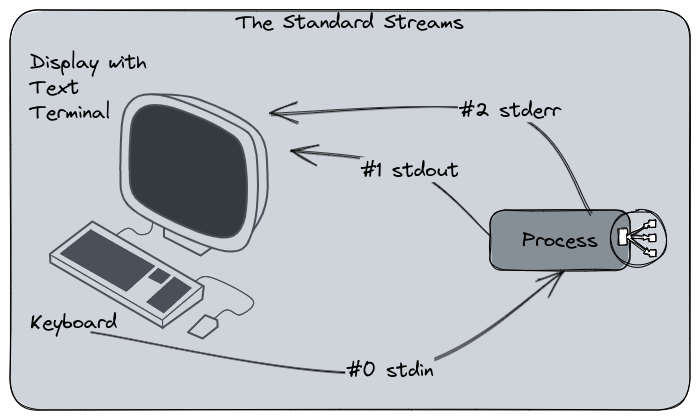
\includegraphics[width=10cm]{image/standard-stream-computer}
    \end{frame}

    \begin{frame}{Commandes de base}{Les flux standards dans le Shell Linux\cref{standard-stream}}
        \centering
        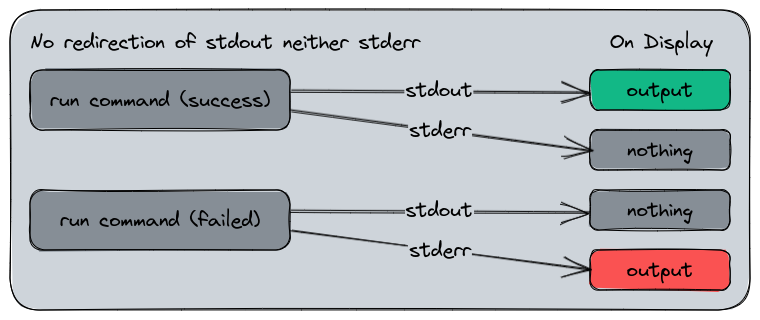
\includegraphics[width=10cm]{image/shell-stream-no-redirect}
    \end{frame}

    \begin{frame}{Commandes de base}{Opérateurs de redirection et piping\footnote{Five ways to use redirect operators in Bash, \url{https://www.redhat.com/sysadmin/redirect-operators-bash}}}
        \begin{itemize}
            \item \lstinline{>}~: Redirige la sortie standard vers un fichier.
            \item \lstinline{>>}~: Redirige la sortie standard vers un fichier en ajoutant le contenu à la fin.
            \item \lstinline{<}~: Redirige un fichier vers l'entrée standard.
            \item \lstinline{2>}~: Redirige la sortie d'erreur vers un fichier.
            \item \lstinline{|}~: Piping, redirige la sortie standard d'une commande vers l'entrée standard d'une autre.
        \end{itemize}
        À quoi ces opérateurs peuvent-ils servir~?
        \begin{center}
            
\includegraphics[width=3cm]{image/question-mark}
        \end{center}
    \end{frame}

    \begin{frame}{Commandes de base}{Exercice \execcounterdispinc{}~:}
        Le but est de créer un fichier source d'un script Shell en y ajoutant ligne par ligne les commandes~:
        \begin{itemize}
            \item Initier la création d'un script Shell nommé \lstinline{discover.sh} dans votre \textquote{home} avec un commentaire descriptif.
            \item Afficher un message indiquant que le \textquote{current working directory} va s'afficher.
            \item Afficher le \textquote{current working directory}.
            \item Afficher un message indiquant que les fichiers et répertoires du répertoire courant vont s'afficher.
            \item Afficher la liste des fichiers et répertoires du répertoire courant.
        \end{itemize}

        Inutile donc indispensable~:
        \begin{itemize}
            \item Changer de répertoire pour aller dans le répertoire courant avec le pipe.
        \end{itemize}
    \end{frame}

    \begin{frame}{Commandes de base}{Exercice \execcounterdispinc{}~:}
        \begin{itemize}
            \item Rediriger la sortie standard standard de la commande \lstinline{ls} dans un fichier \lstinline{ls-output.txt}.
            \item Rediriger la sortie d'erreur error de la commande \lstinline{ls} dans un fichier \lstinline{ls-error.txt}.
            \item Rediriger les deux flux dans un fichier \lstinline{ls-output-error.txt}.
            \item Rediriger le contenu du fichier \lstinline{ls-output.txt} dans la entrée standard de la commande \lstinline{grep} pour filter sur un type d'extension de fichier.
        \end{itemize}
    \end{frame}

    \subsection{Commandes de traitement de données}\label{subsec:commandes-donnees}

    \begin{frame}{Commandes de traitement de données}{Les grands classiques}
        \begin{itemize}
            \item \lstinline{grep}~: Recherche de chaînes de caractères dans un fichier à l'aide d'une RegExp, une \textquote{Regular Expression}.
            Le nom vient de \textit{Global Regular Expression Print}.
            \item \lstinline{sed}~: Stream EDitor, éditeur de flux, permet de modifier le contenu d'un fichier.
            Le plus souvent à l'aide d'une RegExp également.
            Il peut substituer un pattern, supprimer une ligne, ajouter une ligne, \textit{etc}.
            \item \lstinline{awk}~: Traitement de texte, permet de lire un fichier ligne par ligne et de le traiter.
            Il est plus complexe, il a son propre langage de programmation.
            \item \lstinline{cut}~: Permet de découper un fichier en colonnes et de les sélectionner.
            \item \lstinline{sort}~: Trie les lignes d'un fichier.
            \item \lstinline{join}~: Joint les lignes de deux fichiers sur un champ commun.
        \end{itemize}
    \end{frame}

    \subsubsection{Piping}\label{subsubsec:piping}
    \begin{frame}{Commandes de traitement de données}{L'histoire du piping}
        Les opérateurs de redirection et le piping fonctionnent toujours évidement avec ces commandes.
        \bigbreak
        \begin{columns}
            \centering
            \column{0.2\textwidth}
            
\includegraphics[width=3cm]{image/digicomp-video}
            \column{0.8\textwidth}
            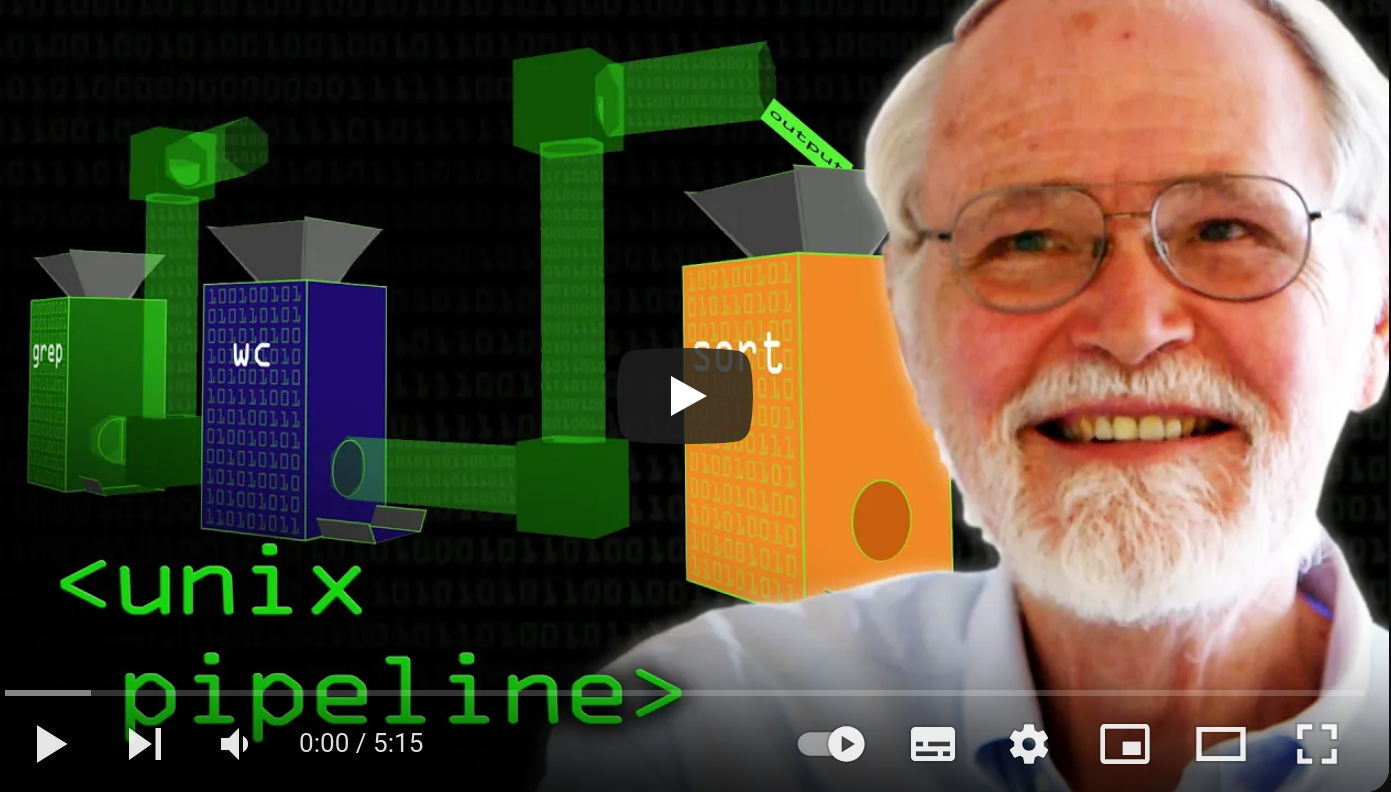
\includegraphics[width=9cm]{image/kernighan-piping-video} \\ \url{https://www.youtube.com/watch?v=bKzonnwoR2I} \\
        \end{columns}
    \end{frame}

    \subsubsection{grep}\label{subsubsec:grep}
    \begin{frame}[fragile]{Commandes de traitement de données}{\lstinline{grep}}
        Par exemple chercher une adresse mail dans un fichier.
        \bigbreak
        On valide d'abord la RegExp en ligne avec un utilitaire comme \url{https://regex101.com/}.
        \bigbreak
        Par exemple, pour chercher les connexions depuis une IP dans le fichier de ProFTP (un serveur FTP)~:
        \begin{lstlisting}[language=bash,basicstyle=\tiny\ttfamily]
$ grep -P 'from\s([0-9]{1,3}.[0-9]{1,3}.[0-9]{1,3}.[0-9]{1,3})' proftpd.log.1
2023-03-05 11:35:16,736 vps19562 proftpd[663168] vps19562.dreamhostps.com (104.156.155.30[104.156.155.30]): USER anonymous: no such user found from 104.156.155.30 [104.156.155.30] to~::ffff:66.33.201.239:21
2023-03-05 13:44:22,711 vps19562 proftpd[664214] vps19562.dreamhostps.com (183.127.77.34.bc.googleusercontent.com[34.77.127.183]): USER anonymous: no such user found from 183.127.77.34.bc.googleusercontent.com [34.77.127.183] to~::ffff:66.33.201.239:21
2023-03-05 21:18:51,926 vps19562 proftpd[669957] vps19562.dreamhostps.com (182.176.228.148[182.176.228.148]): USER local: no such user found from 182.176.228.148 [182.176.228.148] to~::ffff:66.33.201.239:21
2023-03-05 21:59:46,174 vps19562 proftpd[670340] vps19562.dreamhostps.com (107.150.102.211[107.150.102.211]): USER anonymous: no such user found from 107.150.102.211 [107.150.102.211] to~::ffff:66.33.201.239:21
2023-03-06 13:36:11,788 vps19562 proftpd[681605] vps19562.dreamhostps.com (116.62.233.35.bc.googleusercontent.com[35.233.62.116]): USER anonymous: no such user found from 116.62.233.35.bc.googleusercontent.com [35.233.62.116] to~::ffff:66.33.201.239:21
2023-03-07 10:19:49,666 vps19562 proftpd[695638] vps19562.dreamhostps.com (116.62.233.35.bc.googleusercontent.com[35.233.62.116]): USER anonymous: no such user found from 116.62.233.35.bc.googleusercontent.com [35.233.62.116] to~::ffff:66.33.201.239:21
        \end{lstlisting}
    \end{frame}

    \begin{frame}[fragile]{Commandes de traitement de données}{\lstinline{grep} pour le \textquote{Pattern Matching}}
        En rajouter l'option \lstinline{-o} pour avoir uniquement le pattern qui match~:
        \begin{lstlisting}[language=bash]
$ grep -oP 'from\s(\d{1,3}.\d{1,3}.\d{1,3}.\d{1,3})' proftpd.log.1
from 104.156.155.30
from 183.127.77.34
from 182.176.228.148
from 107.150.102.211
from 116.62.233.35
from 116.62.233.35
        \end{lstlisting}
        Uniquement sur les 10 premières lignes grâce à \lstinline{head}~:
        \begin{lstlisting}[language=bash]
$ grep -oP 'from\s(\d{1,3}.\d{1,3}.\d{1,3}.\d{1,3})' <(head -n 10 proftpd.log.1)
from 104.156.155.30
from 183.127.77.34
from 182.176.228.148
from 107.150.102.211
        \end{lstlisting}
        Expliquer cette dernière commande.
    \end{frame}

    \subsubsection{sed}\label{subsubsec:sed}
    \begin{frame}[fragile]{Commandes de traitement de données}{\lstinline{sed} la substitution}
        \lstinline{sed} a son propre langage de programmation avec \lstinline{s/} entre autre\footnote{\label{sed}Sed - An Introduction and Tutorial by Bruce Barnett, \url{https://www.grymoire.com/Unix/Sed.html}}.
        \bigbreak
        On peut anonymiser le fichier en remplaçant une chaine de caractère par une autre.
        \begin{lstlisting}[language=bash,basicstyle=\tiny\ttfamily]
$ head -n 3 proftpd.log.1
2023-03-05 00:17:11,880 vps19562 proftpX[653589] vps19562.dreamhostps.com: ProFTPD 1.3.6c (maint) (built Thu Feb 27 2020 19:34:56 UTC) standalone mode STARTUP
2023-03-05 00:47:51,132 vps19562 proftpX[653845] vps19562.dreamhostps.com (aurora.probe.onyphe.net[142.4.218.114]): USER anonymous: no such user found from aurora.probe.onyphe.net [142.4.218.114] to~::ffff:66.33.201.239:21
2023-03-05 00:55:14,666 vps19562 proftpX[655268] vps19562.dreamhostps.com (hodson.probe.onyphe.net[178.32.197.87]): USER anonymous: no such user found from hodson.probe.onyphe.net [178.32.197.87] to~::ffff:66.33.201.239:21
$ head -n 3 proftpd.log.1 | sed s/vps19562.dreamhostps.com/XXX/
2023-03-05 00:17:11,880 vps19562 proftpX[653589] XXX: ProFTPD 1.3.6c (maint) (built Thu Feb 27 2020 19:34:56 UTC) standalone mode STARTUP
2023-03-05 00:47:51,132 vps19562 proftpX[653845] XXX (aurora.probe.onyphe.net[142.4.218.114]): USER anonymous: no such user found from aurora.probe.onyphe.net [142.4.218.114] to~::ffff:66.33.201.239:21
2023-03-05 00:55:14,666 vps19562 proftpX[655268] XXX (hodson.probe.onyphe.net[178.32.197.87]): USER anonymous: no such user found from hodson.probe.onyphe.net [178.32.197.87] to~::ffff:66.33.201.239:21
        \end{lstlisting}
    \end{frame}

    \begin{frame}[fragile]{Commandes de traitement de données}{\lstinline{sed} la substitution avec \lstinline{s/}\cref{sed}}
        Pour anonymiser le fichier en remplaçant une chaine de caractère par une autre.
        On peut utiliser \lstinline{sed} pour substituer un pattern, donc une RegExp, avec l'option \lstinline{-E}, par une chaîne de caractère et donc anonymiser le fichier en remplaçant les IPv4 par \textquote{xxx.xxx.xxx.xxx}~:
        \begin{lstlisting}[language=bash,basicstyle=\tiny\ttfamily]
$ head -n 3 proftpd.log.1 | sed -E 's/\[[0-9]{1,3}.[0-9]{1,3}.[0-9]{1,3}.[0-9]{1,3}\]/[xxx.xxx.xxx.xxx]/g'
2023-03-05 00:17:11,880 vps19562 proftpX[653589] vps19562.dreamhostps.com: ProFTPD 1.3.6c (maint) (built Thu Feb 27 2020 19:34:56 UTC) standalone mode STARTUP
2023-03-05 00:47:51,132 vps19562 proftpX[653845] vps19562.dreamhostps.com (aurora.probe.onyphe.net[xxx.xxx.xxx.xxx]): USER anonymous: no such user found from aurora.probe.onyphe.net [xxx.xxx.xxx.xxx] to~::ffff:66.33.201.239:21
2023-03-05 00:55:14,666 vps19562 proftpX[655268] vps19562.dreamhostps.com (hodson.probe.onyphe.net[xxx.xxx.xxx.xxx]): USER anonymous: no such user found from hodson.probe.onyphe.net [xxx.xxx.xxx.xxx] to~::ffff:66.33.201.239:21
        \end{lstlisting}
    \end{frame}

    \begin{frame}[fragile]{Commandes de traitement de données}{\lstinline{sed} la supression avec \lstinline{/d}\cref{sed}}
        De la même manière et avec les mêmes options on peut supprimer une ligne qui match une chaine de caractère ou une RegExp~:
        \begin{lstlisting}[language=bash,basicstyle=\tiny\ttfamily]
$ head -n 3 proftpd.log.1
2023-03-05 00:17:11,880 vps19562 proftpX[653589] vps19562.dreamhostps.com: ProFTPD 1.3.6c (maint) (built Thu Feb 27 2020 19:34:56 UTC) standalone mode STARTUP
2023-03-05 00:47:51,132 vps19562 proftpX[653845] vps19562.dreamhostps.com (aurora.probe.onyphe.net[142.4.218.114]): USER anonymous: no such user found from aurora.probe.onyphe.net [142.4.218.114] to~::ffff:66.33.201.239:21
2023-03-05 00:55:14,666 vps19562 proftpX[655268] vps19562.dreamhostps.com (hodson.probe.onyphe.net[178.32.197.87]): USER anonymous: no such user found from hodson.probe.onyphe.net [178.32.197.87] to~::ffff:66.33.201.239:21
$ head -n 3 proftpd.log.1 | sed -E '/\[[0-9]{1,3}.[0-9]{1,3}.[0-9]{1,3}.[0-9]{1,3}\]/d'
2023-03-05 00:17:11,880 vps19562 proftpX[653589] vps19562.dreamhostps.com: ProFTPD 1.3.6c (maint) (built Thu Feb 27 2020 19:34:56 UTC) standalone mode STARTUP
$ head -n 3 proftpd.log.1 | sed '/vps19562.dreamhostps.com/d'
        \end{lstlisting}
        Il peut aussi supprimer une ligne spécifique, par exemple ici la première~:
        \begin{lstlisting}[language=bash,basicstyle=\tiny\ttfamily]
$ head -n 3 proftpd.log.1 | sed '1d'
2023-03-05 00:47:51,132 vps19562 proftpX[653845] vps19562.dreamhostps.com (aurora.probe.onyphe.net[142.4.218.114]): USER anonymous: no such user found from aurora.probe.onyphe.net [142.4.218.114] to~::ffff:66.33.201.239:21
2023-03-05 00:55:14,666 vps19562 proftpX[655268] vps19562.dreamhostps.com (hodson.probe.onyphe.net[178.32.197.87]): USER anonymous: no such user found from hodson.probe.onyphe.net [178.32.197.87] to~::ffff:66.33.201.239:21
        \end{lstlisting}
    \end{frame}

    \begin{frame}[fragile]{Commandes de traitement de données}{\lstinline{sed} plusieurs traitements}
        Plusieurs traitements peuvent être enchainés en les séparant par \lstinline{;}.
        Comme ici avec la suppression de la première ligne et l'anonymisation du serveur ensuite~:
        \begin{lstlisting}[language=bash,basicstyle=\tiny\ttfamily]
$ head -n 3 proftpd.log.1
2023-03-05 00:17:11,880 vps19562 proftpX[653589] vps19562.dreamhostps.com: ProFTPD 1.3.6c (maint) (built Thu Feb 27 2020 19:34:56 UTC) standalone mode STARTUP
2023-03-05 00:47:51,132 vps19562 proftpX[653845] vps19562.dreamhostps.com (aurora.probe.onyphe.net[142.4.218.114]): USER anonymous: no such user found from aurora.probe.onyphe.net [142.4.218.114] to~::ffff:66.33.201.239:21
2023-03-05 00:55:14,666 vps19562 proftpX[655268] vps19562.dreamhostps.com (hodson.probe.onyphe.net[178.32.197.87]): USER anonymous: no such user found from hodson.probe.onyphe.net [178.32.197.87] to~::ffff:66.33.201.239:21
$ head -n 3 proftpd.log.1 | sed -E '1d;s/\] .*.com/] XXX/g'
2023-03-05 00:47:51,132 vps19562 proftpX[653845] XXX (aurora.probe.onyphe.net[142.4.218.114]): USER anonymous: no such user found from aurora.probe.onyphe.net [142.4.218.114] to~::ffff:66.33.201.239:21
2023-03-05 00:55:14,666 vps19562 proftpX[655268] XXX (hodson.probe.onyphe.net[178.32.197.87]): USER anonymous: no such user found from hodson.probe.onyphe.net [178.32.197.87] to~::ffff:66.33.201.239:21
        \end{lstlisting}
    \end{frame}

    \subsubsection{cut}\label{subsubsec:cut}
    \begin{frame}[fragile]{Commandes de traitement de données}{\lstinline{cut} pour gérer les colonnes}
        Il est très utile pour travailler avec les fichiers de données comme CSV, TSV~.

        Il les découpe en colonne et permet de sélectionner les colonnes voulues sur la base d'un séparateur spécifié avec l'option \lstinline{-d} ou \lstinline{--delimiter}.
        \bigbreak
        \lstinline{-f 1,3} pour sélectionner les colonnes 1 et 3~:
        \begin{lstlisting}[language=bash,basicstyle=\tiny\ttfamily]
$ head -n 3 employee.csv
"id";"name";"age";"salary";"dept_id"
0;"John";30;1000;0
1;"Jane";25;1500;0
$ cut employee.csv -f 1,3 --delimiter=';' | head -n 3
"id";"age"
0;30
1;25
        \end{lstlisting}
        \lstinline{-f 1,3} pour sélectionner les colonnes de 1 à 3~:
        \begin{lstlisting}[language=bash,basicstyle=\tiny\ttfamily]
$ cut employee.csv -f 1-3 --delimiter=';' | head -n 3
"id";"name";"age"
0;"John";30
1;"Jane";25
        \end{lstlisting}
    \end{frame}

    \subsubsection{sort}\label{subsubsec:sort}
    \begin{frame}[fragile]{Commandes de traitement de données}{\lstinline{sort} pour trier les lignes}
        \lstinline{sort} trie les lignes d'un fichier en se basant sur le premier champ par défaut ou en spécifiant un champ avec l'option \lstinline{-k} ou \lstinline{--key}.
        \begin{lstlisting}[language=bash,basicstyle=\tiny\ttfamily]
$ head employee.csv -n 4
"id";"name";"age";"salary";"dept_id"
0;"John";30;1000;0
1;"Jane";25;1500;0
2;"Doe";35;2000;1
        \end{lstlisting}
        Pour trier sur le salaire, la colonne 4, séparée par \textquote{;}~:
        \begin{lstlisting}[language=bash,basicstyle=\tiny\ttfamily]
$ sed 1d employee.csv | sort -k 4 --field-separator=';' | head -n 4
0;"John";30;1000;0
1;"Jane";25;1500;0
3;"Steeve";40;2000;0
2;"Doe";35;2000;1
        \end{lstlisting}
        Pour trier sur le salaire puis sur le nom en colonne 2~:
        \begin{lstlisting}[language=bash,basicstyle=\tiny\ttfamily]
$ sed 1d employee.csv | sort -k 4,2 --field-separator=';' | head -n 4
0;"John";30;1000;0
1;"Jane";25;1500;0
2;"Doe";35;2000;1
3;"Steeve";40;2000;0
        \end{lstlisting}
    \end{frame}

    \subsubsection{join}\label{subsubsec:join}
    \begin{frame}[fragile]{Commandes de traitement de données}{\lstinline{join} pour joindre 2 fichiers sur une clé}
        Jointure des fichiers CSV \lstinline{employee.csv} et \lstinline{dept.csv} sur la colonne \lstinline{dept_id} qui est commune aux 2~:
        \begin{lstlisting}[language=bash,basicstyle=\tiny\ttfamily]
$ join -1 1 -2 1 -t ';' -a 2 <(sed 1d employee.csv | sort -k 1 --field-separator=';') <(sed 1d dept.csv | sort -k 1 --field-separator=';')
0;"John";30;1000;0;"HR"
1;"Jane";25;1500;0;"Engineering"
2;"Doe";35;2000;1;"Finance"
$ join -1 1 -2 1 -t ';' -a 1 <(sed 1d employee.csv | sort -k 1 --field-separator=';') <(sed 1d dept.csv | sort -k 1 --field-separator=';')
0;"John";30;1000;0;"HR"
1;"Jane";25;1500;0;"Engineering"
2;"Doe";35;2000;1;"Finance"
3;"Steeve";40;2000;0
4;"Smith";40;2500;1
5;"Brown";45;3000;2
        \end{lstlisting}
        \begin{dangercolorbox}
            Les 2 doivent avoir exactement le même nombre de ligne~!
            Les 3 dernières lignes ont une correspondance dans le fichier \lstinline{dept.csv} mais aucune association n'est faite, car le fichier \lstinline{dept.csv} n'a que 3 lignes.

            Les clés d'associations doivent être triées, il y a donc toujours une étape avec \lstinline{sort} auparavant.
        \end{dangercolorbox}
    \end{frame}

    \begin{frame}{Commandes de traitement de données}{\lstinline{awk}}
        L'histoire et le bien fondé de \lstinline{awk} (12 premières minutes).
        \bigbreak
        \begin{columns}
            \centering
            \column{0.2\textwidth}
            
\includegraphics[width=3cm]{image/digicomp-video}
            \column{0.8\textwidth}
            
\includegraphics[width=9cm]{image/coffee-with-bk} \\ \url{https://www.youtube.com/watch?v=GNyQxXw_oMQ} \\
        \end{columns}
    \end{frame}

    \begin{frame}{Commandes de traitement de données}{\lstinline{awk}}
        \begin{itemize}
            \item \textquote{The right tool for a job}.
            \item N'est même pas packagé, il vient dans toute les distributions.
            \item Data orientated.
            \item Search a matching pattern.
            \item Add numbers.
            \item One liner.
            \item Fonctionne avec des \textquote{associative arrays}, donc similaire à des maps, dictionnaires\ldots.
        \end{itemize}
    \end{frame}

    \begin{frame}{Commandes de traitement de données}{\lstinline{awk}, exercice \execcounterdispinc{}~:}
        Mais c'est aussi pour ajouter des nombres sont créateur à dit, on peut donc faire de l'analytique avec~!
        \bigbreak
        Quel la somme des salaires par département dans le fichier \lstinline{employee.csv}~?
        \bigbreak
        \centering
        
\includegraphics[width=3cm]{image/question-mark}
    \end{frame}

    \subsubsection{Exercice}\label{subsubsec:data-exercice}
    \begin{frame}{Commandes de traitement de données}{Exercice \execcounterdispinc{}~:}
        Cet exercice a pour objectif d'illustrer qu'un prétraitement avec ces commandes est efficace.
        Plus qu'un équivalent SQL~.
        \bigbreak
        Il est courant de limiter les données en base SQL aux besoins des programmes haut-niveau, d'un backend Java, CoBOL, PHP par exemple, pour ne pas surcharger les serveurs SQL~.
        \bigbreak
        Ces commandes ne remplacent pas SQL, car elles s'interfacent difficilement avec ces programmes haut-niveau.
        \bigbreak
        Par contre, elles peuvent traiter des flux de données avant de les mettre en base.
        L'exercice consiste à développer avec ces commandes l'équivalent des \href{https://github.com/DigicompClassesByPapIT/linux2/blob/main/sqlite-hr.sh}{traitements SQL de ce fichier}.

        Analyser~:
        \begin{itemize}
            \item Ce qui peut être qualifié d'\textquote{efficace}.
            \item Ce que cette \textquote{efficacité} apporte à l'entreprise.
            \item Quelle version SQL ou Shell est la plus sensible aux bugs et pourquoi~?
        \end{itemize}
    \end{frame}

    \subsubsection{Equivalence SQL - Shell}\label{subsubsec:equi-sql-shell}
    \begin{frame}{Commandes de traitement de données}{Equivalence SQL - Shell}
        De nombreux traitements de données ne nécessitent pas toujours de SQL, ils ont leur équivalent en Shell~:
        \begin{table}[ht]
            \centering
            \begin{tabular}{|c|c|}
                \hline
                \textbf{SQL}         & \textbf{Shell}                   \\
                \hline
                \lstinline{SELECT}   & \lstinline{cut}                  \\
                \hline
                \lstinline{DELETE}   & \lstinline{sed}                  \\
                \hline
                \lstinline{UPDATE}   & \lstinline{sed}, \lstinline{awk} \\
                \hline
                \lstinline{INSER}    & \lstinline{<}                    \\
                \hline
                \lstinline{WHERE}    & \lstinline{grep}                 \\
                \hline
                \lstinline{JOIN}     & \lstinline{awk}                  \\
                \hline
                \lstinline{GROUP BY} & \lstinline{awk}                  \\
                \hline
                \lstinline{SORT BY}  & \lstinline{sort}                 \\
                \hline
            \end{tabular}
%\caption{SQL functions and their Shell commands equivalents}
        \end{table}
        Dans une grande banque d'investissement française, chaque soir, le data center d'IBM facture des dizaines de milliers d'EUR pour les batchs qui traitent les données du jour\ldots
    \end{frame}

    \subsubsection{Les variantes}\label{subsubsec:variantes}

    \begin{frame}{Commandes de traitement de données}{Variantes de ces outils}
        Ces outils sont open-source et ont d'innombrables variantes~:
        \begin{itemize}
            \item \lstinline{egrep}~: Extended \lstinline{grep}.
            \item \lstinline{gsed}~: La version sous licence GNU de \lstinline{sed}.
            \item \lstinline{gawk}~: La version sous licence GNU de \lstinline{awk}.
            \item \lstinline{bawk}~: \lstinline{bawk}, binary \lstinline{bawk}, pour parser des fichiers binaires.
            \item \lstinline{busybox}~: Ils ont tous une version dans cette boîte à outils.
        \end{itemize}
        \bigbreak
        Quel est l'intérêt de traiter des fichiers binaires~?
        \bigbreak
        \centering
        
\includegraphics[width=3cm]{image/question-mark}
    \end{frame}

    \begin{frame}[fragile]{Commandes de traitement de données}{Variantes de ces outils}
        Dans les exemples précédents, nous n'avons manipulé que des données issues de fichier texte.
        Les données numériques prennent moins de place en binaire.
        \begin{lstlisting}[language=python]
from sys import getsizeof
from struct import pack
print("lentgh of the string:", getsizeof("65535"))
print("lentgh of the struct:", getsizeof(pack(">H", 0xffff)))
lentgh of the string: 46
lentgh of the struct: 35
        \end{lstlisting}
        La valeur d'un octet est comprise entre 0 et 255, mais pour obtenir du texte, on passe par une table de correspondance, un encodage, qui donnera un seul caractère.
        La valeur numérique la plus élevée pour ce même octet en texteb donc 9.
        \bigbreak
        Pour des soucis de performance, de coût (du cloud), il n'est pas rare que les formats de données soit binaires.
    \end{frame}


    \section{Utilisateurs, groupes et droits d'accès}\label{sec:utilisateurs-groupes-droits}

    \subsection{Groupes}\label{subsec:groupes}

    \begin{frame}{Utilisateurs, groupes et droits d'accès}{Les groupes}
        \begin{columns}
            \column{0.5\textwidth}
            Les groupes facilitent la gestion des droits d'accès.
            En effet, il est plus simple de gérer les droits d'accès pour un groupe d'utilisateurs que pour chaque utilisateur.
            \bigbreak
            L'administrateur a tout intérêt à créer des groupes pour les utilisateurs qui ont les mêmes besoins et par la même, diminuer le nombre de droits à gérer et les erreurs possibles.
            \column{0.5\textwidth}
            \centering
            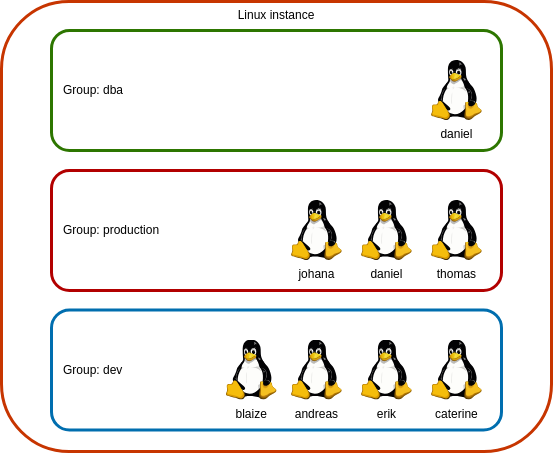
\includegraphics[width=6cm]{image/groups-and-users.drawio}
        \end{columns}
    \end{frame}

    \begin{frame}[fragile]{Utilisateurs, groupes et droits d'accès}{Les groupes}
        L'utilitaire \lstinline{addgroup} permet de créer un groupe.
%bash listing
        \begin{lstlisting}[language=bash]
$ whoami
chrichri
$ addgroup digicomp
fatal: Seul le superutilisateur est autorisé à ajouter un utilisateur ou un groupe au système.
        \end{lstlisting}
        Pourquoi cela ne fonctionne pas~?
        \pause
        \begin{dangercolorbox}
            Pour ajouter un groupe, il faut être superutilisateur.
            C'est à dire, avoir les droits \textquote{root}.
            Donc être \textquote{root}, ou utiliser \lstinline{sudo}, si on est \textquote{sudoer}, \textit{i.e.}, que l'on fait partie du groupe \textquote{sudo}.
        \end{dangercolorbox}
        \begin{lstlisting}[language=bash]
$ sudo addgroup digicomp
info: Choix d'un GID dans la plage 1000 à 59999 ...
info: Ajout du groupe « digicomp » (GID 1002)...
$ groups
chrichri adm dialout cdrom sudo audio dip video plugdev lpadmin pulse lxd sambashare docker libvirt nordvpn
$ members sudo
chrichri
$ members digicomp
        \end{lstlisting}
    \end{frame}

    \begin{frame}[fragile]{Utilisateurs, groupes et droits d'accès}{Les groupes}
        \lstinline{groups} permet de lister les groupes auxquels appartient un utilisateur, mais aussi de lister tous les groupes~:
        \begin{lstlisting}[language=bash]
$ groups chrichri
chrichri~: chrichri adm dialout cdrom sudo audio dip video plugdev lpadmin pulse lxd sambashare nordvpn docker libvirt
        \end{lstlisting}
        \lstinline{members} permet de lister les membres d'un groupe.
        Il nous confirme que le groupe \lstinline{digicomp} est bien créé.
        Il n'a pas de membre.
        \bigbreak
        Pour qu'une ressource, fichier, dossier, appartienne à un groupe, il faut que le groupe soit propriétaire de la ressource.
        Pour cela, la commande \lstinline{chown}(CHange OWNer) permet de changer le propriétaire d'une ressource.
% Shell listing
        \begin{lstlisting}[language=bash]
$ mkdir digicomp-little-secret
$ touch digicomp-little-secret/secret.txt
$ echo "Le code de l'entrée est 8564" > digicomp-little-secret/secret.txt
$ cat digicomp-little-secret/secret.txt
Le code de l'entrée est 8564
$ sudo chown root:digicomp -R digicomp-little-secret/
$ ls -lha digicomp-little-secret/
total 12K
drwxrwxr-x  2 root     digicomp 4,0K août  15 16:07 .
drwxrwxr-x 10 chrichri chrichri 4,0K août  15 16:07 ..
-rw-rw-r--  1 root     digicomp   29 août  15 16:08 secret.txt
        \end{lstlisting}
    \end{frame}

    \begin{frame}[fragile]{Utilisateurs, groupes et droits d'accès}{Les groupes}
        \lstinline{sudo chown root:digicomp -R digicomp-little-secret} veut dire que le groupe propriétaire de \lstinline{digicomp-little-secret} est \lstinline{digicomp} et de manière récursive, \textit{i.e.}, pour les sous-dossiers et fichiers.
        La structure de la commande est \lstinline{chown <user>:<group> -R <path>}.
        Et il faut là aussi être \textquote{superutilisateur}, ici avec \lstinline{sudo}.
        \bigbreak
        Mais\ldots
        \begin{lstlisting}[language=bash]
$ cat digicomp-little-secret/secret.txt
Le code de l'entré est 8564
$ echo "Le code de l'entré est 2539" > digicomp-little-secret/secret.txt
bash: digicomp-little-secret/secret.txt: Permission non accordée
        \end{lstlisting}
        Qu'est-ce que cela veut dire~?
        \begin{center}
            
\includegraphics[width=3cm]{image/question-mark}
        \end{center}
    \end{frame}

    \subsection{Droits}\label{subsec:droits}

    \begin{frame}{Utilisateurs, groupes et droits d'accès}{Les droits\footnote{\label{rights-digitalocean}An Introduction to Linux Permissions, \url{https://www.digitalocean.com/community/tutorials/an-introduction-to-linux-permissions}}}
        \begin{dangercolorbox}
            Cela montre que des users qui ne sont pas prioritaires et qui ne font pas partie du groupe propriétaire peuvent avoir des droits.
            Par défaut ces droits sont en lecture seule, n'ont n'avons pas pu écrire dans le fichier.
        \end{dangercolorbox}
        \centering
        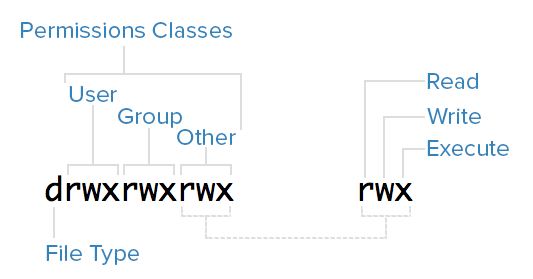
\includegraphics[width=7cm]{image/permission-classes}
        \flushleft
        Les droits par défaut du fichier en question étaient \lstinline{-rw-rw-r--}.
    \end{frame}

    \begin{frame}[fragile]{Utilisateurs, groupes et droits d'accès}{Les droits\cref{rights-digitalocean}}
        \begin{lstlisting}[language=bash]
$ ls -lha digicomp-little-secret/
total 12K
drwxrwxr-x  2 root     digicomp 4,0K août  15 16:07 .
drwxrwxr-x 10 chrichri chrichri 4,0K août  15 16:07 ..
-rw-rw-r--  1 root     digicomp   29 août  15 16:08 secret.txt
        \end{lstlisting}
        \begin{columns}
            \column{0.4\textwidth}
            N'étant ni dans le groupe propriétaire, ni propriétaire, l'utilisateur \lstinline{chrichri} est autre, ses droits sont donc \lstinline{r--}.

            Qui veut dire, \textit{read} uniquement.
            Ce qui est cohérent avec les commandes précédentes.
            \column{0.6\textwidth}
            \begin{center}
                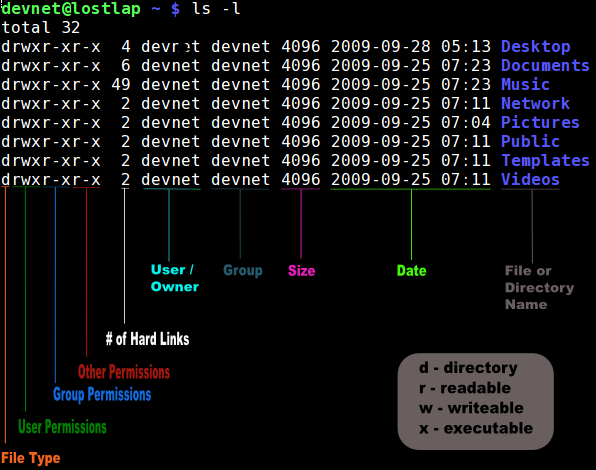
\includegraphics[width=6.5cm]{image/ls-details}
            \end{center}
        \end{columns}
    \end{frame}

    \begin{frame}{Utilisateurs, groupes et droits d'accès}{Les droits\cref{rights-digitalocean}\footnotestep\footnote{\label{octal}Octal Notation and Linux Permissions, \url{https://cratecode.com/info/octal-notation}}}
        \begin{columns}
            \column{0.5\textwidth}
            La notation octale est une manière de représenter les droits d'accès.
            \bigbreak
            \textit{In fine}, c'est un nombre qui est la concaténation de 3 suites de valeurs binaires\ldots.
            \column{0.5\textwidth}
            \begin{center}
                
\includegraphics[width=6.5cm]{image/binary-explosion}
            \end{center}
        \end{columns}
    \end{frame}

    \begin{frame}[fragile]{Utilisateurs, groupes et droits d'accès}{Représentation binaire la notation octale avec Python\cref{octal}}
        \begin{lstlisting}
int("000", 2) # Masque binaire de 3 de longs donc 0 est le minimum
Out[30]: 0
int("111", 2) # 7 le maximum, de 0 à 7 il y a 8 valeurs d'où octal
Out[31]: 7
int("001", 2) # Execute: --x
Out[32]: 1
int("010", 2) # Write: -w-
Out[33]: 2
int("100", 2) # Read: r--
Out[34]: 4
int("110", 2) # Read/write: rw-
Out[35]: 6
int("111", 2) # Read/write/execute: rwx
Out[36]: 7
int("011", 2) # Write/execute: -wx
Out[37]: 3
int("101", 2) # Write/execute: w-x
Out[38]: 5
        \end{lstlisting}
    \end{frame}

    \begin{frame}[fragile]{Utilisateurs, groupes et droits d'accès}{Notation octale\cref{octal}}
        Cela fait bien des droits qui vont de 0 pour la lecture seule au user, à 777 pour la lecture, l'écriture et l'exécution au user, groupe et autres.
        \begin{lstlisting}
"".join(map(str, [int("100", 2), int("000", 2), int("000", 2)])) # r-- pour user
Out[46]: '400'
"".join(map(str, [int("111", 2), int("111", 2), int("111", 2)])) # rwx pour tous
Out[45]: '777'
        \end{lstlisting}
        Ces droits s'appliquent avec la commande \lstinline{chmod} pour CHange MODe.
        Selon le format suivant \lstinline{chmod <mode> <file>}.
        \lstinline{<mode>} étant le chiffre calculé entre 000 et 777 calculé au dessus.
        Comme pour \lstinline{chown}, l'option \lstinline{-R} peut être ajoutée pour être récursif dans les sous-dossiers et fichiers.
        \bigbreak
        Des utilitaires de validation de cette notation, plus user friendly que Python, sont en ligne comme \url{https://chmod-calculator.com/}.
    \end{frame}

    \begin{frame}[fragile]{Utilisateurs, groupes et droits d'accès}{Notation octale\cref{octal}}
        En résumé, restreindre les droits à la lecture par l'utilisateur propriétaire m'empêche de lire le fichier~:
        \begin{lstlisting}[language=bash]
$ sudo chmod 400 digicomp-little-secret/secret.txt
$ cat digicomp-little-secret/secret.txt
cat: digicomp-little-secret/secret.txt: Permission non accordée
        \end{lstlisting}
        Graĉe à \lstinline{sudo} je peux me donner les droits en lecture ou écriture par exemple~:
        \begin{lstlisting}[language=bash]
$ sudo chmod 007 digicomp-little-secret/secret.txt
$ cat digicomp-little-secret/secret.txt
Le code de l'entrée est 8564
$ sudo chmod 002 digicomp-little-secret/secret.txt
$ cat digicomp-little-secret/secret.txt
cat: digicomp-little-secret/secret.txt: Permission non accordée
$ echo "Le code de l'entrée est 8564" > digicomp-little-secret/secret.txt
        \end{lstlisting}
    \end{frame}

    \subsection{Utilisateurs}\label{subsec:utilisateurs}
    \begin{frame}{Utilisateurs, groupes et droits d'accès}{Les utilisateurs}
        Les utilisateurs sont les personnes qui utilisent le système.
        Les bonnes pratiques veulent qu'il y en a un par personne physique.
        L'utilisateur a pour s'identifier un user et un mot de passe et/ou une clé privé.
        C'est l'administrateur du système qui lui génère son premier mot de passe et sa première clé.
        Un user peut faire partie de plusieurs groupes, comme ici \lstinline{daniel} qui est \lstinline{dba} et \lstinline{prod}.
        \begin{columns}
            \column{0.5\textwidth}
            Exemple de commandes pour gérer un utilisateur~:
            \begin{itemize}
                \item \lstinline{adduser}~: Ajouter un utilisateur.
                \item \lstinline{passwd}~: Changer le mot de passe.
                \item \lstinline{usermod}~: Modifier un utilisateur.
                \item \lstinline{userdel}~: Supprimer un utilisateur.
            \end{itemize}
            \column{0.5\textwidth}
            \centering
            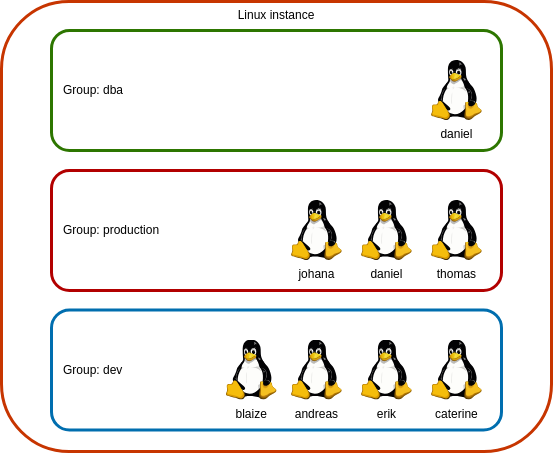
\includegraphics[width=5cm]{image/groups-and-users.drawio}
        \end{columns}
    \end{frame}

    \begin{frame}[fragile]{Utilisateurs, groupes et droits d'accès}{Les utilisateurs}
        Exemple avec la création du user \lstinline{digiformateur}.
        \begin{lstlisting}[language=bash]
$ useradd -s /bin/bash -m -d $/home/digiformateur digiformateur
useradd: Permission denied.
useradd~: impossible de vérouiller /etc/passwd ; réessayer plus tard.
$ sudo useradd -s /bin/bash -m -d $/home/digiformateur digiformateur # sudo
$ passwd digiformateur
passwd~: Vous ne devriez pas voir ou modifier l'information du mot de passe pour digiformateur.
$ sudo passwd digiformateur # superutilisateur
Nouveau mot de passe~: 
Retapez le nouveau mot de passe~: 
passwd~: mot de passe mis à jour avec succès
$ su digiformateur
Mot de passe~: 
$ whoami
digiformateur
$ exit
exit
$ userdel digiformateur # superutilisateur
userdel: Permission denied.
userdel~: impossible de vérouiller /etc/passwd ; réessayer plus tard.
$ sudo userdel digiformateur
        \end{lstlisting}
    \end{frame}

    \subsection{Mot de passe}\label{subsec:password}
    \begin{frame}{Utilisateurs, groupes et droits d'accès}{Recommandation sur les motrs de passe}
        \begin{footnotesize}
            Bonnes pratiques de l'ANSSI\footnote{Bonnes pratiques - Protégez-vous~!, \url{https://cyber.gouv.fr/bonnes-pratiques-protegez-vous}} pour les mots de passe~:
            \begin{columns}
                \column{0.5\textwidth}
                \begin{itemize}
                    \item Créer un mot de passe suffisamment long, complexe et inattendu~:
                    de 8 caractères minimum et contenant des minuscules, des majuscules,
                    des chiffres et des caractères spéciaux.

                    \item Ne communiquez jamais votre mot de passe à un tiers~: aucune
                    organisation ou personne de confiance ne vous demandera de lui
                    communiquer votre mot de passe.

                \end{itemize}
                \column{0.6\textwidth}
                \centering
                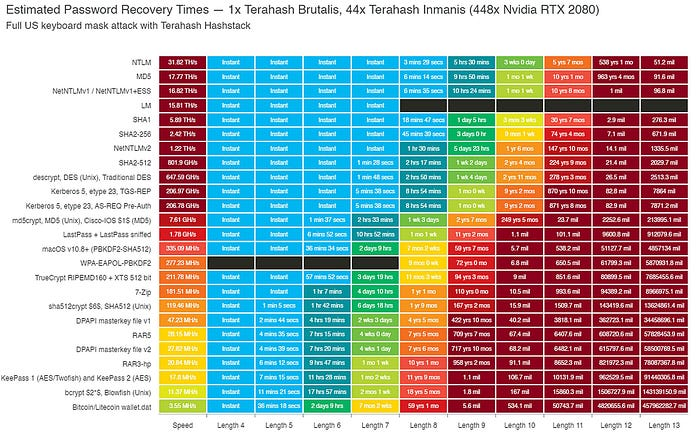
\includegraphics[width=6.5cm]{image/real-password-cracking} \\ Hashcat benchmark\footnotemark \\
            \end{columns}
            Mais le mot de passe seul n'est pas suffisant, le plus sûr reste le SSH avec la paire de clés privé et publique.
            \footnotetext{Those Tables With Password Cracking Times That Scare You And Peddle Snake Oil — Are Mostly Wrong!, \url{https://billatnapier.medium.com/those-tables-password-cracking-times-that-scare-you-are-mostly-wrong-7d03bf4aec6}}
        \end{footnotesize}
    \end{frame}

    \subsection{Exercice}\label{subsec:user-group-rights-exercice}
    \begin{frame}{Utilisateurs, groupes et droits d'accès}{Exercice \execcounterdispinc}
        Cet exercice a pour objectif de montrer que les droits d'accès sont une question de sécurité, les configurations et les services sont très sensibles.
        En effet, les services sont le plus souvent exécutés par l'utilisateur root et ont donc le maximum de droits.
        \bigbreak
        Il est courant de donner des droits en lecture seule à un fichier de configuration, mais de ne pas donner de droits en écriture.
        \begin{itemize}
            \item Créer un user qui aura des droits en écriture sur la configuration d'un service dans \lstinline{/etc/systemd/system}.
            \item Créer un groupe qui aura des droits en écriture sur la configuration d'un autre service dans \lstinline{/etc/systemd/system}.
            \item Ajouter à ce dernier groupe le nouveau user.
            \item Supprimer groupe et user.
            \item Remettre les droits comme avant sur les deux services.
        \end{itemize}
    \end{frame}

    \begin{frame}{Utilisateurs, groupes et droits d'accès}{Exercice \execcounterdispinc}
        Cet exercice a pour objectif de créer un simple site web static isolé par le jeu des user/groupes/droits.
        \begin{itemize}
            \item Créer un groupe pour ce serveur/site web.
            \item Créer un user type développeur qui aura des droits adéquats sur un dossier et fichier \lstinline{/var/www/html/digicomp/index.html}.
            \item Créer un user type production qui aura des droits adéquats sur un dossier et fichier \lstinline{/var/www/html/digicomp/index.html}.
            \item Un script shell à exécuter grâce au shebang \lstinline{\#!/bin/bash} qui lance la commande Python \lstinline{python3 -m http.server -d /var/www/html/digicomp/}.
            Ce script shell ne peut être exécuté par l'utilisateur de production uniquement et aucune resource ne doit pouvoir être modifiée.
        \end{itemize}
    \end{frame}


    \section{Système de fichiers}\label{sec:fs}
    \begin{frame}{Système de fichiers}{Définition\footnote{\label{fs}Les systèmes de fichiers sous GNU-Linux / macOS / Windows, \url{https://doc.ubuntu-fr.org/systeme_de_fichiers}}}
        \begin{footnotesize}
            Soft qui organise les fichiers de votre ordinateur sur votre disque dur de façon
            à pouvoir les retrouver lorsque vous en avez besoin.
            Les systèmes de fichiers les plus répandus à l'heure actuelle sont sûrement le FAT32 et
            le NTFS, qui sont les deux seuls systèmes de fichiers que Microsoft® Windows® peut nativement lire.
            Il existe de nombreux autres systèmes de fichiers~: ext2, ext3, ext4, ReiserFS, JFS, XFS, Btrfs, ZFS\ldots
            \begin{table}[h!]
                \centering
                \begin{tabular}{|c|c|c|c|c|}
                    \hline
                    \textbf{Nom} & \textbf{Fichier max} & \textbf{Partition max} & \textbf{Journalisé} & \textbf{Gestion des droits} \\ \hline
                    BtrFS        & 16 EiB               & 16 EiB                 & Non (CoW)           & Oui                         \\ \hline
                    exFAT        & 16 TiB               & 256 TiB                & Oui                 & Oui                         \\ \hline
                    ext2FS       & 2 TiB                & 4 TiB                  & Non                 & Oui                         \\ \hline
                    ext3FS       & 2 TiB                & 4 TiB                  & Oui                 & Oui                         \\ \hline
                    ext4FS       & 16 TiB               & 1 EiB                  & Oui                 & Oui                         \\ \hline
                    FAT          & 2 GiB                & 2 GiB                  & Non                 & Non                         \\ \hline
                    FAT32        & 4 GiB                & 8 TiB                  & Non                 & Non                         \\ \hline
                    NTFS         & 16 TiB               & 256 TiB                & Oui                 & Oui                         \\ \hline
                    ReiserFS     & 8 TiB                & 16 TiB                 & Oui                 & Oui                         \\ \hline
                    UDF          & 16 EiB               & 2 To                   & Non                 & Oui                         \\ \hline
                \end{tabular}
            \end{table}
        \end{footnotesize}
    \end{frame}

    \begin{frame}[fragile]{Système de fichiers}{Définition\cref{fs}}
        Sans cette indexation, il serait impossible de retrouver un fichier sur un disque dur.
        Qui n'est que une immensité de données binaires~:
        \begin{lstlisting}
$ sudo dd if=/dev/nvme0n1p3 ibs=512 count=1 skip=239 2> /dev/null | hexdump -C
00000000  00 d7 01 d7 02 d7 03 d7  04 d7 05 d7 06 d7 07 d7  |................|
00000010  08 d7 09 d7 0a d7 0b d7  0c d7 0d d7 0e d7 0f d7  |................|
00000020  10 d7 11 d7 12 d7 13 d7  14 d7 15 d7 16 d7 17 d7  |................|
00000030  18 d7 19 d7 1a d7 1b d7  1c d7 1d d7 1e d7 1f d7  |................|
00000040  20 d7 21 d7 22 d7 23 d7  24 d7 25 d7 26 d7 27 d7  | .!.".#.$.%.&.'.|
00000050  28 d7 29 d7 2a d7 2b d7  2c d7 2d d7 2e d7 2f d7  |(.).*.+.,.-.../.|
00000060  30 d7 31 d7 32 d7 33 d7  34 d7 35 d7 36 d7 37 d7  |0.1.2.3.4.5.6.7.|
00000070  38 d7 39 d7 3a d7 3b d7  3c d7 3d d7 3e d7 3f d7  |8.9.:.;.<.=.>.?.|
        \end{lstlisting}
        \lstinline{dd} est une commande qui permet de lire et écrire tout ou partie d'un disque
        \bigbreak
        Par défaut sur les machines Ubuntu le système de fichier est \lstinline{ext4}.
        \bigbreak
        Mais ZFS est aussi supporté.
        Il est plus courant sur les serveurs qui stock des données, plus que sur les serveurs applicatifs.
    \end{frame}

    \begin{frame}{Système de fichiers}{Du hardware au Kernel\footnote{Linux File System\url{https://www.javatpoint.com/linux-file-system}}}
        \centering
        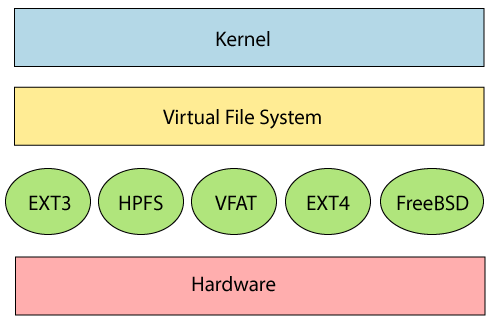
\includegraphics[width=11cm]{image/linux-file-system-stack}
    \end{frame}

    \subsection{Montage du système de fichiers}\label{subsec:mount}
    \begin{frame}[fragile]{Système de fichiers}{Comment rajouter un disque~?}
        \begin{scriptsize}
            \begin{itemize}
                \item \lstinline{lsblk}~: Pour lister les disques et les partitions.
                \item \lstinline{parted}~: Pour lister et modifier les disques et les partitions.
                \item \lstinline{mount}~: Pour monter le disque.
                \item \lstinline{df}~: Pour vérifier que le disque est bien monté.
            \end{itemize}
            \begin{lstlisting}[language=bash,basicstyle=\tiny\ttfamily]
$ sudo parted -l
Modèle~: KPART512GBC2DVT (nvme)
Disque /dev/nvme0n1~: 512GB
Taille des secteurs (logiques/physiques)~: 512B/512B
Table de partitions~: gpt
Drapeaux de disque~:

Numéro  Début   Fin    Taille  Système de fichiers  Nom                           Drapeaux
 1      1049kB  211MB  210MB   fat32                EFI system partition          démarrage, esp
 2      211MB   228MB  16,8MB                       Microsoft reserved partition  msftres
 3      228MB   129GB  129GB   ntfs                 Basic data partition          msftdata
 4      129GB   233GB  104GB   ntfs                 Basic data partition          msftdata
 8      233GB   491GB  258GB   ext4


Modèle~: Inconnu (unknown)
Disque /dev/zram0~: 8271MB
Taille des secteurs (logiques/physiques)~: 4096B/4096B
Table de partitions~: loop
Drapeaux de disque~:

Numéro  Début  Fin     Taille  Système de fichiers  Drapeaux
 1      0,00B  8271MB  8271MB  linux-swap(v1)
            \end{lstlisting}
        \end{scriptsize}
    \end{frame}

    \begin{frame}{Système de fichiers}{Comment rajouter un disque~?}
        Combien de disque(s) physique(s) \lstinline{parted} a-t-il indiqué~?
        \begin{center}
            
\includegraphics[width=3cm]{image/question-mark}
        \end{center}
        \pause
        \begin{dangercolorbox}
            Il y a un seul disque physique, \lstinline{/dev/nvme0n1}.

            L'autre est la RAM, une partie du système de fichier, celle dédiée aux fichiers temporaires est mappée sur la RAM pour des soucis de performance.
        \end{dangercolorbox}
    \end{frame}

    \begin{frame}[fragile]{Système de fichiers}{Comment rajouter un disque~?}
        \begin{scriptsize}
            En connectant un nouveau disque on constate bien avec \lstinline{parted} qu'il y a un nouveau disque~:
            \begin{lstlisting}[basicstyle=\tiny\ttfamily]
Modèle~: Intuix DiskOnKey (scsi)
Disque /dev/sda~: 252MB
Taille des secteurs (logiques/physiques)~: 512B/512B
Table de partitions~: loop
Drapeaux de disque~:

Numéro  Début  Fin    Taille  Système de fichiers  Drapeaux
 1      0,00B  252MB  252MB   ext4
            \end{lstlisting}
            4 To environ au format NTFS, il est sous \lstinline{/dev/sda}.
            A-t-il un point de montage sur le système de fichier~?
            \begin{lstlisting}[language=bash,basicstyle=\tiny\ttfamily]
$ df
Sys. de fichiers        blocs de 1K   Utilisé Disponible Uti% Monté sur
tmpfs                       1615420      6264    1609156   1% /run
/dev/nvme0n1p8            247090272 199514156   34951836  86% /
tmpfs                       8077096     11248    8065848   1% /dev/shm
tmpfs                          5120         8       5112   1% /run/lock
efivarfs                        184       172          8  96% /sys/firmware/efi/efivars
tmpfs                       8077096         0    8077096   0% /run/qemu
tmpfs                       2097152      3400    2093752   1% /tmp
/dev/nvme0n1p1               200704     51428     149276  26% /boot/efi
tmpfs                       1615416      2596    1612820   1% /run/user/1000
/home/chrichri/.Private   247090272 199514156   34951836  86% /home/chrichri/Private
            \end{lstlisting}
        \end{scriptsize}
    \end{frame}

    \begin{frame}[fragile]{Système de fichiers}{Comment rajouter un disque~?}
        Créons un \textquote{point de montage} et montons ce disque~:
        \begin{lstlisting}[language=bash]
$ sudo mkdir /mnt/sda-usb # /mnt pour les montage par convention mais peut être ailleurs
$ sudo mkfs.ext4 /dev/sda # formatage du disque en Ext4 car le FS était incompatible
$ sudo mount /dev/sda /mnt/sda-usb
$ ls /mnt/sda-usb -lha
total 24K
drwxr-xr-x 3 root root 4,0K août  17 15:21 .
drwxr-xr-x 5 root root 4,0K août  17 15:08 ..
drwx------ 2 root root  16K août  17 15:21 lost+found
        \end{lstlisting}
        \begin{dangercolorbox}
            \lstinline{mkfs.ext4} est une commande qui permet de formater un disque en Ext4.
            Elle supprime donc les données du disque.
            Elle est néanmoins nécessaire pour pouvoir monter le disque, il y avait en effet une incompatibilité de système de fichier.
            Ces incompatibilités sont fréquentes avec les systèmes de fichiers Windows® comme FAT et NTFS~.
        \end{dangercolorbox}
    \end{frame}

    \begin{frame}[fragile]{Système de fichiers}{Comment rajouter un disque~?}
        Comme ces commandes ont été exécutées par le supersaturation, il est probable ques les droits bloque l'écriture~:
        \begin{lstlisting}[language=bash]
$ cp ocr_speed.txt /mnt/sda-usb
cp: impossible de créer le fichier standard '/mnt/sda-usb/ocr_speed.txt': Permission non accordée
$ sudo cp ocr_speed.txt /mnt/sda-usb
$ sudo chown chrichri: -R /mnt/sda-usb
$ sudo chmod 700 /mnt/sda-usb
$ cp ocr_speed.txt /mnt/sda-usb
$ /mnt/sda-usb/ocr_speed.txt -lha
-rw-r--r-- 1 chrichri chrichri 212 août  17 15:37 /mnt/sda-usb/ocr_speed.txt
        \end{lstlisting}
        Des modifications ont pu être apportées.
        \bigbreak
        Avant de retirer le disque peut démonter le disque et éventuellement supprimer le point de montage~:
        \begin{lstlisting}[language=bash]
$ sudo umount /dev/sda
$ ls /mnt/sda-usb
$ sudo rm -rf /mnt/sda-usb
        \end{lstlisting}
    \end{frame}

    \begin{frame}{Système de fichier}{Exercice \execcounterdispinc}
        \newcounter{exemountcounter}
        \setcounter{exemountcounter}{\value{execounter}}
        % add one as execounter not incremented yet
        \addtocounter{exemountcounter}{1}
        Cet exercice a pour objectif d'ajouter un disque en lecture seule sur votre Bureau.
        \begin{itemize}
            \item Le disque est une clé USB pluggée à votre PC~.
            \item Créer le point de montage sur le bureau.
            \item Montez-y la clé USB~.
            Après l'avoir démonter si elle a été montée automatiquement par l'OS~.
            \item Modifier les droits pour qu'elle soit en lecture seule.
            \item Démonter la clé USB~.
            \item Supprimer le point de montage.
        \end{itemize}
        \bigbreak
        \centering
        
\includegraphics[width=3cm]{image/guy-in-front-of-desktop}
    \end{frame}

    \subsection{La table du système de fichiers (/etc/fstab)}\label{subsec:fstab}
    \begin{frame}[fragile]{Système de fichiers}{La table du système de fichiers (\lstinline{/etc/fstab})}
        \lstinline{/etc/fstab} est un fichier de configuration associe des points de montage à des disques.
        Il est lu au démarrage du système pour monter les disques automatiquement et ne pas avoir à passer les commandes vues précédemment.
        \bigbreak
        Il permet également de configurer des partitions spécialisées comme \lstinline{/tmp} ou \lstinline{swapfile}.
        \begin{lstlisting}[language=bash,basicstyle=\tiny\ttfamily]
$ cat /etc/fstab
# /etc/fstab: static file system information.
#
# Use 'blkid' to print the universally unique identifier for a
# device; this may be used with UUID= as a more robust way to name devices
# that works even if disks are added and removed. See fstab(5).
#
# <file system> <mount point>   <type>  <options>       <dump>  <pass>
# / was on /dev/nvme0n1p8 during installation
UUID=9bcc82ee-9214-4eac-90f6-9695c585874b /               ext4    errors=remount-ro 0       1
# /boot/efi was on /dev/nvme0n1p1 during installation
UUID=EE30-267D  /boot/efi       vfat    umask=0077      0       1
#/swapfile                                 none            swap    sw              0       0
# Temp file in memory.
tmpfs /tmp tmpfs defaults,size=2G 0 0
        \end{lstlisting}
    \end{frame}

    \begin{frame}[fragile]{Système de fichiers}{La table du système de fichiers (\lstinline{/etc/fstab})}
        \lstinline{/etc/fstab} est un fichier de configuration associe des points de montage à des disques.
        On y trouve les UUID des disques, le point de montage, le type de système de fichier, les options de montage du disque principale~:
        \begin{lstlisting}[basicstyle=\tiny\ttfamily]
UUID=9bcc82ee-9214-4eac-90f6-9695c585874b /               ext4    errors=remount-ro 0       1
        \end{lstlisting}
        La partition de boot montée sur \lstinline{/boot/efi}~:
        \begin{lstlisting}[basicstyle=\tiny\ttfamily]
UUID=EE30-267D  /boot/efi       vfat    umask=0077      0       1
        \end{lstlisting}
        La \lstinline{swapfile} qui est commentée pour car c'est une extension de la RAM sur le disque, c'est configuration invite l'OS à utiliser un maximum la RAM~.
        La partition \lstinline{/tmp} montée en mémoire pour de meilleurs performances avec certaines commandes comme \lstinline{sort}, la mémoire est plus rapide que le SSD.~:
        \begin{lstlisting}[basicstyle=\tiny\ttfamily]
# Temp file in memory.
tmpfs /tmp tmpfs defaults,size=2G 0 0
        \end{lstlisting}
        On peut aussi utiliser ce fichier pour configurer le montage au moment du démarrage d'un disque supplémentaire, clé USB sur un point de montage~:
        \begin{lstlisting}[basicstyle=\tiny\ttfamily]
# /boot was on /dev/sda5 during installation
/dev/sda5                                    /boot           ext2    defaults          0       2
        \end{lstlisting}
    \end{frame}

    \begin{frame}{Système de fichiers}{Exercices de configuration de la table du système de fichiers (\lstinline{/etc/fstab})}
        Exercice \execcounterdispinc: Reprendre les consignes de l'exercice  \theexemountcounter{} et ajouter le disque à la table du système de fichiers \lstinline{/etc/fstab} pour que la clé soit montée automatiquement au démarrage.
        \bigbreak
        Exercice \execcounterdispinc: Créer un disque virtuel de 1 Go et le monter automatiquement au démarrage en configurant \lstinline{/etc/fstab}.
        \bigbreak
        \centering
        
\includegraphics[width=3cm]{image/guy-in-front-of-desktop}
    \end{frame}

    \subsection{RAID}\label{subsec:raid}

    \begin{frame}{RAID}{Les différents RAID\footnote{\label{mdadm}mdadm~: RAID Logiciel sous Linux, \url{https://www.linuxtricks.fr/wiki/mdadm-raid-logiciel-sous-linux}}\footnotestep\footnote{Qu'est-ce que le RAID ?, \url{https://www.diskpart.com/fr/windows-server/logiciel-gestion-raid-8899-tc.html}}}
        Le RAID est un ensemble de standards de virtualisation du stockage permettant de répartir des données sur plusieurs disques durs afin d'améliorer soit les performances, soit la sécurité ou la tolérance aux pannes de l'ensemble du ou des systèmes.
        \bigbreak
        \centering
        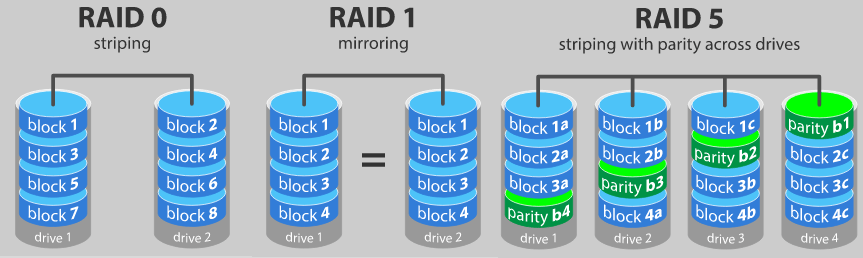
\includegraphics[width=10cm]{image/raid-0-1-5} \\ Les principaux RAID, les 0, 1 et 5 \\
    \end{frame}

    \begin{frame}{RAID}{\lstinline{mdadm}\cref{mdadm}\footnotestep\footnote{RAID logiciel avec mdadm, \url{https://doc.ubuntu-fr.org/raid_logiciel}}}
        \begin{itemize}
            \item Logiciel installable sous Ubuntu avec le package manager, pas besoin de compilation.
            \item Comme pour les autres commandes \textquote{bas-niveau}, elle nécessite d'être superutilisateur.
            \item Il lance un service qui monitor les processus nécessaires au RAID~.
            Un service se lance automatiquement au démarrage du système.
            \item Il faut que les disques soient vierges, sinon les données seront perdues.
            \item Il est recommandé qu'ils aient la même taille, mais ce n'est pas indispensable.
            Dans le cas contraire, l'espace dédié au RAID sera de la taille du plus petit disque et le reste sera non-RAID~.
            \item Ajout de disques dit \textquote{spare} ou en français dormants, qui ne sont pas utilisés par le RAID tant qu'un autre disque n'est pas tombé en panne.
        \end{itemize}
    \end{frame}

    \begin{frame}{RAID}{RAID logiciel ou controller RAID hardware?}
        \begin{itemize}
            \item Le RAID logiciel est plus flexible, car il est indépendant du matériel.
            Surtout si le controller n'est une carte du type PCIe mais qu'il est intégré à la carte mère.
            \item Le RAID hardware est plus performant, car il est géré par un processeur dédié.
            Le software prend des ressources qui pourraient être utilisées par d'autres softwares.
            \item Le RAID hardware est plus cher, car il nécessite un contrôleur RAID~.
            \item Le RAID hardware est plus difficile à maintenir.
            \item Un Contrôleurs RAID Intel® coûtent 100 à 700 CHF~.
        \end{itemize}
    \end{frame}

    \begin{frame}{RAID}{Exercice \execcounterdispinc{}}
        L'objectif est de maîtriser les commandes de base de l'outil \lstinline{mdadm}\cref{mdadm}.
        \begin{itemize}
            \item Créer 2 disques vierges de 1 Go chacun.
            \item Lancer la VM Ubuntu avec les 2 disques créés.
            \item Se connecter à la VM~.
            \item Vérifier l'ajout des 2 disques avec une commande vue précédemment.
            \item Suivre le tutorial \url{https://www.linuxtricks.fr/wiki/mdadm-raid-logiciel-sous-linux} pour créer un RAID 1.
        \end{itemize}
        \bigbreak
        \centering
        
\includegraphics[width=3cm]{image/guy-in-front-of-desktop}
    \end{frame}

    \begin{frame}{RAID}{Exercice \execcounterdispinc{}}
        Quel est un des dangers de RAID 0?
        \bigbreak
        \centering
        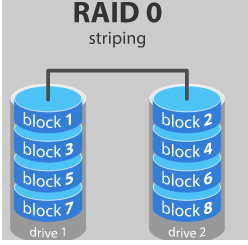
\includegraphics[width=5cm]{image/raid-0}
    \end{frame}

    \subsection{LVM}\label{subsec:lvm}

    \begin{frame}{Logical Volume Manager, A.K.A LVM}{Définition\footnote{\label{lvm}LVM, une autre manière de partitionner, \url{https://doc.ubuntu-fr.org/lvm}}}
        Il permet la création et la création de volumes logiques.
        Ces derniers sont des partitions virtuelles qui peuvent être agrandies ou réduites sans perte de données.
        Et sont décorrélées des disques physiques (les PV ou \textquote{Physical Volume}).
        \bigbreak
        Un ou plusieurs PV sont regroupés en un ou plusieurs VG \textquote{Volume group}.
        \bigbreak
        C'est dans ces VG que sont créés les LV \textquote{Logical Volume} qui remplacent les partitions.
        \bigbreak
        Un des bénéfices est qu'un dossier comme par exemple \lstinline{/var/lib/mysql} qui contient les données de la base MySQL peut être plus grand qu'un disque physique entier~!
    \end{frame}

    \begin{frame}{Logical Volume Manager, A.K.A LVM}{Définition\cref{lvm}}
        \centering
        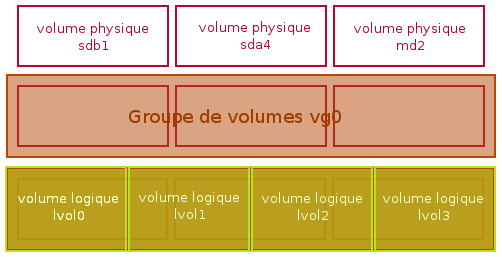
\includegraphics[width=10cm]{image/lvm}
        \flushleft
        Le PV peut être un disque RAID, par sécurité, pour prévenir une perte de données c'est même conseillé.
    \end{frame}

    \begin{frame}{Logical Volume Manager, A.K.A LVM}{Définition\cref{lvm}}
        Si les données sont strippées (avec les options \lstinline{-I} et/ou \lstinline{-i} de \lstinline{lvm2}\footnote{Analysing a Standard Logical Volume, \url{https://www.theurbanpenguin.com/striped-lvm-volumes/}}) le risque de perte de données est plus grand sans RAID mais la performance est meilleure comme avec RAID 0.
        \bigbreak
        \begin{columns}
            \column{0.5\textwidth}
            L'idéale en terme de sécurité et de performance est d'avoir un RAID 1 pour les PV et les volumes logiques strippées.
            \bigbreak
            Par défaut, avec la commande \lstinline{mount}, le montage configuré sera perdu au redémarrage.
            Une configuration de \lstinline{/etc/fstab} permet de garder le montage du LV après redémarrage.
            \column{0.5\textwidth}
            \bigbreak
            \centering
            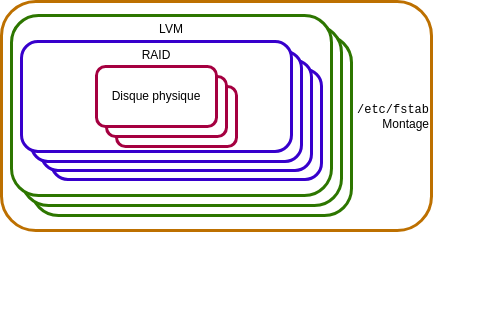
\includegraphics[width=7cm]{image/fs-stack.drawio}
        \end{columns}
    \end{frame}

    \begin{frame}{Système de fichier}{Exercice \execcounterdispinc}
        Avec le disque RAID créé précédemment, il est possible de créer un volume logique avec LVM~.
        \begin{itemize}
            \item Créer un volume physique~.
            \item Créer un groupe logique~.
            \item Créer un volume logique~.
            \item Monter le volume logique sur \lstinline{/lib/var/mysql}.
            \item Ajouter le montage du volume logique dans \lstinline{/etc/fstab} pour que le volume se monte au démarrage de la machine.
            \item Redémarrer la machine pour tester.
        \end{itemize}
    \end{frame}


    \section{Processus}\label{sec:processus}

    \subsection{Gestion des processus}\label{subsec:process-management}

    \begin{frame}{Gestion des processus}{Définition\footnote{\label{process}Les processus sous Linux, \url{https://www.cyberciti.biz/faq/how-to-check-running-process-in-ubuntu-linux-using-command-line/}}}
        Un processus est un programme en cours d'exécution.
        Il est identifié par un PID, le \textquote{Process IDentifier}.
        \bigbreak
        Il peut être en cours d'exécution, en attente, en pause, en zombie, dormant ou en terminaison, \textit{etc}.
        Il est possible de voir les processus avec la commande \lstinline{ps} ou \lstinline{top}.
        \bigbreak
        \begin{columns}
            \column{0.7\textwidth}
            \lstinline{ps} affiche les informations de manière statique alors que est dynamique, interactif et temps réel.
            \lstinline{ps} peut donc être utilisé également dans des scripts Shell.

            Les processus peuvent être tués avec la commande \lstinline{kill}.

            Les données les concernant sont stockées dans le dossier \lstinline{/proc}.
            \column{0.3\textwidth}
            \centering
            
\includegraphics[width=4cm]{image/proc-hamster}
        \end{columns}
    \end{frame}

    \begin{frame}[fragile]{Gestion des processus}{Les commandes \lstinline{ps}}
        L'option \lstinline{-f} affiche plus d'informations sur les processus.
        \begin{lstlisting}[language=bash,basicstyle=\tiny\ttfamily]
$ ps
    PID TTY          TIME CMD
 276321 pts/5    00:00:00 bash
 338450 pts/5    00:00:00 ps
$ ps -f
UID          PID    PPID  C STIME TTY          TIME CMD
chrichri  276321  265707  0 13:17 pts/5    00:00:00 /usr/bin/bash --rcfile /home/chrichri/pycharm-professional-2024.1.4/pycharm-2024.1.4/plugins/terminal/shell-integrations/bash/bash-integration.bash -i
chrichri  338508  276321 99 14:12 pts/5    00:00:00 ps -f
        \end{lstlisting}
        Une commande par nom de processus et avec la ligne de commande complète~:
        \begin{lstlisting}[language=bash,basicstyle=\tiny\ttfamily]
$ ps -fC java
UID          PID    PPID  C STIME TTY          TIME CMD
chrichri  265707    8404 80 13:08 ?        00:42:46 /home/chrichri/pycharm...
        \end{lstlisting}
        \bigbreak
        Les processus de l'utilisateur courant~:
        \begin{lstlisting}[language=bash,basicstyle=\tiny\ttfamily]
$ ps -u chrichri
    PID TTY          TIME CMD
   8059 ?        00:00:06 systemd
   8068 ?        00:00:00 (sd-pam)
   8090 ?        00:00:02 pipewire
...
        \end{lstlisting}
        \bigbreak
        Les processus de l'utilisateur courant et de tous les autres utilisateurs, \textit{i.e.}, tous les processus~:
        \begin{lstlisting}[language=bash,basicstyle=\tiny\ttfamily]
$ ps -ef
UID          PID    PPID  C STIME TTY          TIME CMD
root           1       0  0 09:23 ?        00:00:05 /sbin/init splash
root           2       0  0 09:23 ?        00:00:00 [kthreadd]
...
        \end{lstlisting}
    \end{frame}

    \begin{frame}{Gestion des processus}{Les états d'un processus sous \lstinline{ps}}
        \begin{table}[h!]
            \centering
            \begin{tabular}{|p{0.1\textwidth}|p{0.8\textwidth}|}
                \hline
                \textbf{État} & \textbf{Description}                                                                      \\ \hline
                \textbf{D}    & Sommeil ininterrompu (habituellement en attente d'IO)                                     \\ \hline
                \textbf{R}    & En cours d'exécution ou prêt à être exécuté (dans la file d'attente)                      \\ \hline
                \textbf{S}    & Sommeil interruptible (en attente de la complétion d'un événement)                        \\ \hline
                \textbf{T}    & Arrêté, soit par un signal de contrôle de tâche, soit parce qu'il est tracé               \\ \hline
                \textbf{W}    & Pagination (non valide depuis le noyau 2.6.xx)                                            \\ \hline
                \textbf{X}    & Mort (ne devrait jamais être vu)                                                          \\ \hline
                \textbf{Z}    & Processus défunt (\textquote{zombie}), terminé mais non récupéré par son processus parent \\ \hline
            \end{tabular}
            \caption{États des processus sous Linux sous \lstinline{ps}}
        \end{table}
    \end{frame}

    \begin{frame}{Gestion des processus}{L'interface \lstinline{top}}
        La commande \lstinline{top} affiche tous les processus.
        Mais il ne permet pas de trouver les processus par nom contrairement à \lstinline{ps}.
        \bigbreak
        Les principales fonctions que l'on peut appeler dans l'interface~:
        \begin{table}[h!]
            \centering
            \begin{tabular}{|p{0.1\textwidth}|p{0.8\textwidth}|}
                \hline
                \textbf{Touche} & \textbf{Fonction}                           \\ \hline
                \textbf{k}      & Met fin à un processus                      \\ \hline
                \textbf{m}      & Trie la liste par utilisation de la mémoire \\ \hline
                \textbf{n}      & Trie la liste par PID                       \\ \hline
                \textbf{r}      & Modifie la priorité d’un processus          \\ \hline
                \textbf{h}      & Affiche la fenêtre d’aide                   \\ \hline
                \textbf{z}      & Affiche les processus en cours en couleurs  \\ \hline
                \textbf{d}      & Modifie l’intervalle de rafraîchissement    \\ \hline
                \textbf{c}      & Affiche le chemin absolu d’un processus     \\ \hline
                \textbf{f}      & Écran de personnalisation                   \\ \hline
            \end{tabular}
            \caption{États des processus sous Linux sous \lstinline{top}}
        \end{table}
    \end{frame}

    \begin{frame}{Gestion des processus}{Les états d'un processus sous \lstinline{top}}
        \begin{table}[h!]
            \centering
            \begin{tabular}{|p{0.1\textwidth}|p{0.8\textwidth}|}
                \hline
                \textbf{État} & \textbf{Description}                      \\ \hline
                \textbf{D}    & Sommeil ininterrompu                      \\ \hline
                \textbf{I}    & Inactif                                   \\ \hline
                \textbf{R}    & En cours d'exécution                      \\ \hline
                \textbf{S}    & En sommeil                                \\ \hline
                \textbf{T}    & Arrêté par un signal de contrôle de tâche \\ \hline
                \textbf{t}    & Arrêté par un débogueur lors d'un traçage \\ \hline
                \textbf{Z}    & Processus zombie                          \\ \hline
            \end{tabular}
            \caption{États des processus sous Linux sous \lstinline{top}}
        \end{table}
    \end{frame}

    \begin{frame}{Gestion des processus}{L'interface \lstinline{top}}
        Top et \textquote{c} pour afficher la ligne de commande~:
        \bigbreak
        \centering
        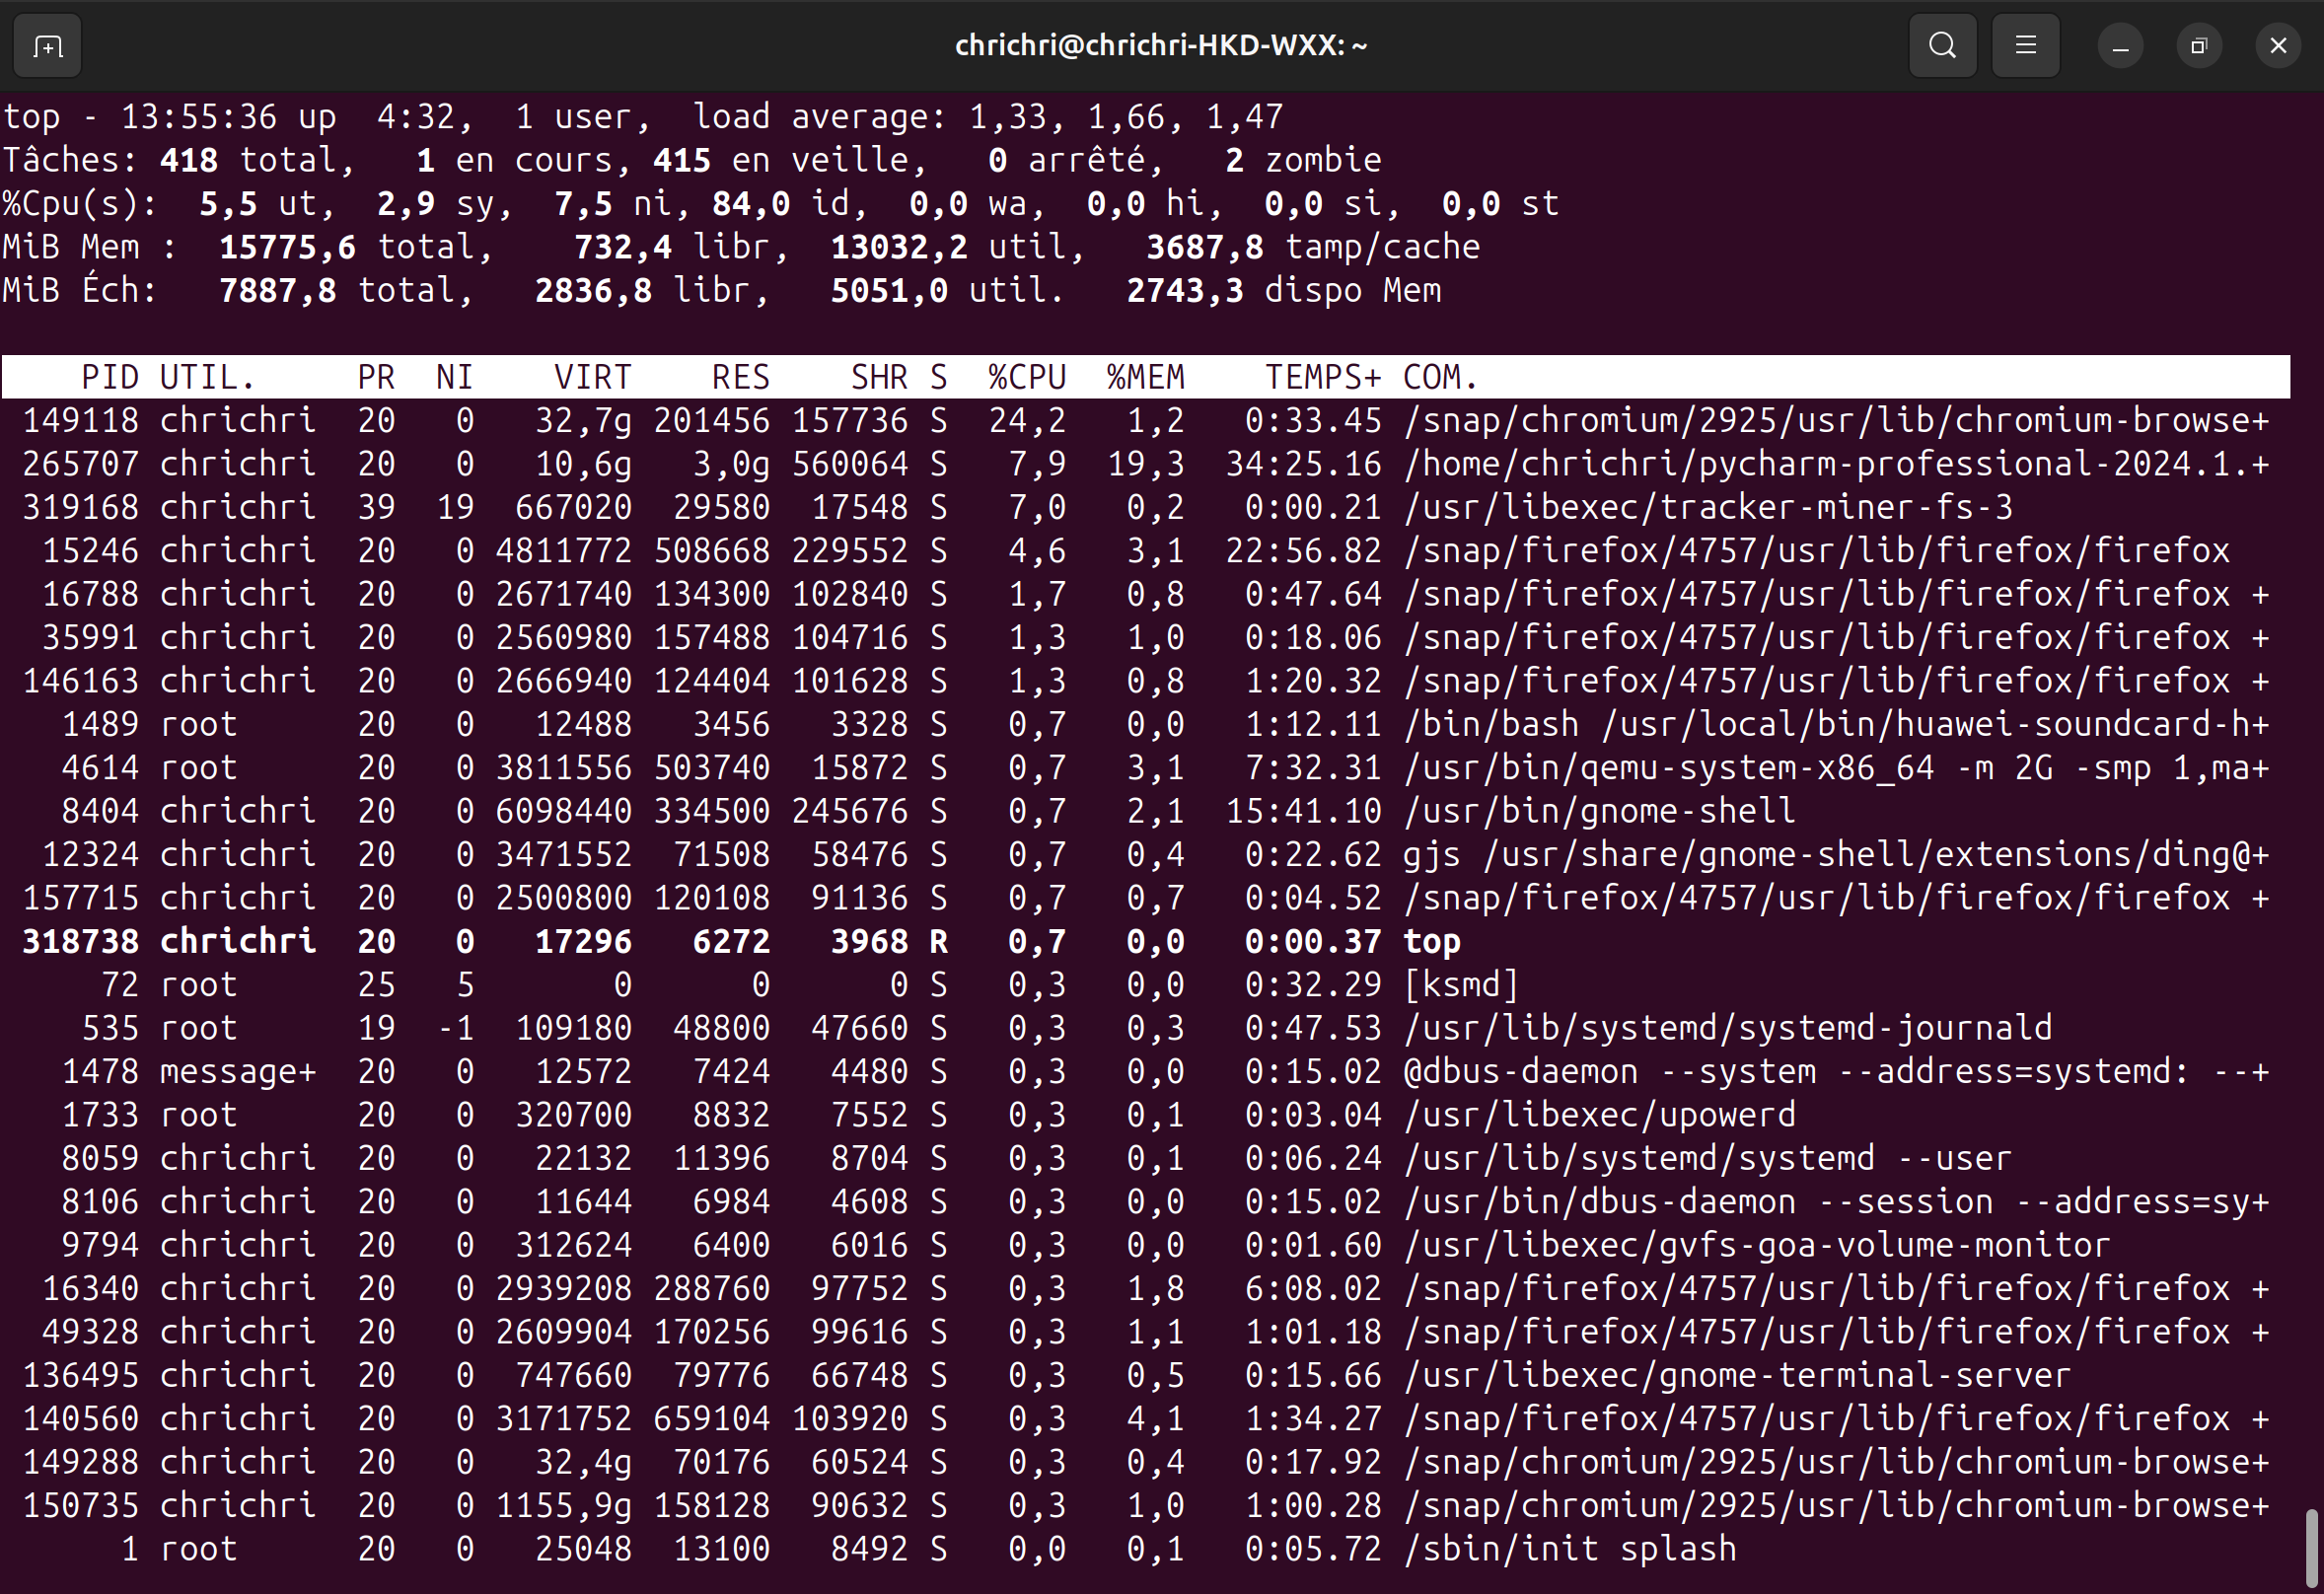
\includegraphics[width=10cm]{image/top-interface}
    \end{frame}

    \begin{frame}[fragile]{Gestion des processus}{La commande \lstinline{kill}}
        La commande \lstinline{top} permet de terminer un processus dans l'interface avec \textbf{k}.
        En fonction de son PID, qu'on aurait auparavant dans cette même interface.
        ou avec la commande \lstinline{ps}, on peut le tuer avec la commande \lstinline{kill}.
        \bigbreak
        Mais il existe une commande spécifique, c'est \lstinline{kill}, elle envoie un signal au processus ici SIGKILL avec l'option \lstinline{-9}.
        Elle permet de terminer un processus dont aurait trouvé le PID avec \lstinline{ps} ou \lstinline{top}.
        \begin{lstlisting}[language=bash]
$ kill -9 <PID>
        \end{lstlisting}
        \bigbreak
        La commande \lstinline{pkill} permet de tuer un processus par son nom, celui qui s'affiche dans \lstinline{ps} ou \lstinline{top}.
        \begin{lstlisting}[language=bash]
$ pkill -9 <nom>
        \end{lstlisting}
    \end{frame}

    \begin{frame}{Gestion des processus}{Le dossier \lstinline{/proc}\footnote{The /proc Filesystem, \url{https://docs.kernel.org/filesystems/proc.html}}}
        \begin{footnotesize}
            Le dossier \lstinline{/proc} contient des informations sur les processus sous l'arborescence de son PID donc \lstinline{/proc/<PID>/} dans les fichiers suivants~:
            \begin{tiny}
                \begin{table}[h!]
                    \centering
                    \begin{tabular}{|p{2cm}|p{8cm}|}
                        \hline
                        \textbf{File}             & \textbf{Content}                                                                                                                \\
                        \hline
                        \lstinline{clear\_refs}   & Clears page referenced bits shown in smaps output                                                                               \\
                        \hline
                        \lstinline{cmdline}       & Command line arguments                                                                                                          \\
                        \hline
                        \lstinline{cpu}           & Current and last cpu in which it was executed (2.4)(smp)                                                                        \\
                        \hline
                        \lstinline{cwd}           & Link to the current working directory                                                                                           \\
                        \hline
                        \lstinline{environ}       & Values of environment variables                                                                                                 \\
                        \hline
                        \lstinline{exe}           & Link to the executable of this process                                                                                          \\
                        \hline
                        \lstinline{fd}            & Directory, which contains all file descriptors                                                                                  \\
                        \hline
                        \lstinline{maps}          & Memory maps to executables and library files (2.4)                                                                              \\
                        \hline
                        \lstinline{mem}           & Memory held by this process                                                                                                     \\
                        \hline
                        \lstinline{root}          & Link to the root directory of this process                                                                                      \\
                        \hline
                        \lstinline{stat}          & Process status                                                                                                                  \\
                        \hline
                        \lstinline{statm}         & Process memory status information                                                                                               \\
                        \hline
                        \lstinline{status}        & Process status in human readable form                                                                                           \\
                        \hline
                        \lstinline{wchan}         & Present with \lstinline{CONFIG\_KALLSYMS=y:} it shows the kernel function symbol the task is blocked in - or “0” if not blocked \\
                        \hline
                        \lstinline{pagemap}       & Page table                                                                                                                      \\
                        \hline
                        \lstinline{stack}         & Report full stack trace, enable via \lstinline{CONFIG\_STACKTRACE}                                                              \\
                        \hline
                        \lstinline{smaps}         & An extension based on maps, showing the memory consumption of each mapping and flags associated with it                         \\
                        \hline
                        \lstinline{smaps\_rollup} & Accumulated smaps stats for all mappings of the process. This can be derived from smaps, but is faster and more convenient      \\
                        \hline
                        \lstinline{numa\_maps}    & An extension based on maps, showing the memory locality and binding policy as well as mem usage (in pages) of each mapping      \\
                        \hline
                    \end{tabular}
                \end{table}
            \end{tiny}
        \end{footnotesize}
    \end{frame}

    \begin{frame}{Système de fichier}{Exercices sur les processus}
        \begin{small}
            Exercice \execcounterdispinc{}, quels droits ai-je \lstinline{/proc} sur les processus des autres utilisateurs~?
            \bigbreak
            Exercice \execcounterdispinc{}, quels droits ai-je \lstinline{/proc} sur mes processus~?
            \bigbreak
            Exercice \execcounterdispinc{}, terminer un processus découvert sous \lstinline{top} avec la commande \lstinline{kill}.
            \bigbreak
            Exercice \execcounterdispinc{}, terminer un processus découvert sous \lstinline{top} avec la commande \lstinline{pkill}.
            \bigbreak
            Personnaliser \lstinline{top} pour que l'interface affiche les processus non pas en pourcentage totale de CPU consommé (par défaut) mais en pourcentage par cœur.
        \end{small}
        \begin{center}
            \includegraphics[width=3cm]{image/guy-in-front-of-desktop}
        \end{center}
    \end{frame}

    \begin{frame}{Système de fichier}{Exercices \execcounterdispinc{}}
        \begin{itemize}
            \item Lancer en arrière plan le script Shell \lstinline{endless-loop.sh}.
            \item Arrêter le processus correspondant au script dans \lstinline{top}.
            \item Lancer à nouveau en arrière plan le script Shell \lstinline{endless-loop.sh}.
            \item Arrêter le processus correspondant au script à l'aide de  \lstinline{ps} et \lstinline{kill}.
        \end{itemize}
        \bigbreak
        \centering
        \includegraphics[width=3cm]{image/guy-in-front-of-desktop}
    \end{frame}

    \begin{frame}{Système de fichier}{Exercices sur les processus}
        Exercices \execcounterdispinc{}, à partir de vos connaissances sur les process et des commandes précédentes comparer l'activité d'une machine Ubuntu, d'un WSL ubuntu et d'un WSL Debian, ou un FreeBSD~.

        Que remarquez-vous~?
        \pause
        \bigbreak
        \centering
        \includegraphics[width=10cm]{image/top-debian} \\ Ubuntu est-il en train de devenir un \textit{bloatware~}, lui aussi\ldots \emoji{window}?
    \end{frame}

    \subsection{Gestion des priorités des processus}\label{subsec:process-priority}

    \begin{frame}{Gestion des Priorités des Processus}{Définition\footnote{\label{process-priority}Linux commands: How to manipulate process priority, \url{https://www.redhat.com/sysadmin/manipulate-process-priority}}}
        \begin{itemize}
            \item Dans un système multi-tâches, plusieurs processus s'exécutent en parallèle.
            \item Le système d'exploitation doit allouer équitablement les ressources (CPU, RAM, \textit{etc}) entre ces processus.
            \item Les priorités permettent de contrôler l'ordonnancement des processus.
            \item Chaque processus a une priorité.
            \item Une priorité plus élevée signifie que le processus recevra plus de temps CPU~.
            \item Sur les systèmes Unix/Linux, la priorité est représentée par une valeur appelée \lstinline{nice}.
            \item Une bonne gestion des priorités est cruciale lors montées en charge du système (scaling).
        \end{itemize}
    \end{frame}

    \begin{frame}{Gestion des Priorités des Processus}{Commande \lstinline{nice}\cref{process-priority}}
        \begin{itemize}
            \item \lstinline{nice} permet de démarrer un processus avec une priorité spécifique.
            \item Syntaxe~: \lstinline{nice -n [valeur] [commande]}.
            \item La valeur de nice varie de -20 (priorité élevée) à 19 (priorité faible).
            \item Exemple~: \lstinline{nice -n 10 myprocess}
            \item On retrouve ce niveau de priorité dans \lstinline{top} avec la colonne \textquote{NI}.
        \end{itemize}
    \end{frame}

    \begin{frame}{Gestion des Priorités des Processus}{Commande \lstinline{renice}\cref{process-priority}}
        \begin{itemize}
            \item \lstinline{renice} modifie la priorité d'un processus en cours d'exécution.
            \item Elle nécessite les droits superutilisateur.
            \item Syntaxe~: \lstinline{renice [valeur] -p [PID]}.
            \item PID (Process ID) est l'identifiant unique du processus.
            \item Utiliser \lstinline{ps} pour trouver le PID du processus.
            \item Exemple~: \lstinline{renice -5 -p 1234}
        \end{itemize}
    \end{frame}

    \begin{frame}[fragile]{Commandes \lstinline{nice} et \lstinline{renice}}{Exemple de commandes}
        Une priorité peut être attribuée au début de l'exécution et modifiée par la suite~:
        \begin{lstlisting}[language=bash]
$ nohup nice -n 15 ./endless-loop.sh & 
[1] 906674
$ nohup: les entrées sont ignorées et la sortie est ajoutée à 'nohup.out'
$ renice -19 -p 906674
renice: échec de configuration de priorité pour 906674 (process ID): Permission non accordée
$ sudo renice -19 -p 906674
906674 process ID) priorité précédente 15, nouvelle priorité -19
        \end{lstlisting}
        \begin{center}
            \includegraphics[width=5cm]{image/pinguins-racing}
        \end{center}
    \end{frame}


    \section{Les services Linux}\label{sec:les-services}

    \begin{frame}{Les services}{Définition}
        \begin{footnotesize}
            Dans les systèmes Windows et Linux, le terme service désigne un programme qui s'exécute en arrière-plan, sans intervention de l'utilisateur.

            Il faut le configurer pour qu'il démarre automatiquement, dans un certain ordre et avec les bonnes permissions.
            \bigbreak
            La configuration principale consiste à définit une ligne de commande qui sera exécutée au démarrage du service.
            \bigbreak
            Avec \lstinline{systemd}\footnote{System and Service Manager, \url{https://systemd.io/}} sous Linux, on peut définir des dépendances entre les services.
            Limiter les ressources CPU, mémoire, IO, \textit{etc}.
            Définir ce qu'il faut faire en cas de crash.
            Exécuter des scripts avant et après le démarrage du service.
            \bigbreak
            Leur chemin par défaut est \lstinline{/etc/systemd/system/}.
            \begin{dangercolorbox}
                Ne pas confondre \lstinline{systemd} qui exécute des tâches en arrière plan et l'ordonnanceur \lstinline{cron}.
            \end{dangercolorbox}
        \end{footnotesize}
    \end{frame}

    \begin{frame}[fragile]{Les services}{Exemples}
        \lstinline{systemd} est donc l'outil de choix pour lancer en production des applications, des progiciels, \textit{etc}.

        Encore mieux, on peut configurer des services pour qu'ils lancent des VM avec Qemu et les applications tourneraient dans les VM~.
        On profite des avantages de la virtualisation pour isoler les applications et les sécuriser.
        \bigbreak
        Que fait cette configuration~?
        \begin{lstlisting}
[Unit]
Description=IN DATA development application
[Service]
RuntimeMaxSec=3600s
Restart=always
WorkingDirectory=/home/debian/dev/IN FRANCE
ExecStart="/home/debian/dev/IN FRANCE/python3-dev/bin/python3" -m gunicorn -w 1 -b unix:/tmp/in-france-dev-indata-gunicorn.sock application_indata
[Install]
WantedBy=multi-user.target
        \end{lstlisting}
        \begin{dangercolorbox}
            Le chemin de l'exécutable dans \lstinline{ExecStart} doit être absolu!
        \end{dangercolorbox}
    \end{frame}

    \begin{frame}{Les services}{Les commandes de base}
        \begin{itemize}
            \item \lstinline{systemctl start <service>} pour démarrer un service.
            \item \lstinline{systemctl stop <service>} pour arrêter un service.
            \item \lstinline{systemctl restart <service>} pour redémarrer un service.
            \item \lstinline{systemctl status <service>} pour afficher le statut d'un service.
            \item \lstinline{systemctl enable <service>} pour activer un service au démarrage.
            \item \lstinline{systemctl disable <service>} pour désactiver un service au démarrage.
            \item \lstinline{systemctl list-units --type=service} pour lister les services.
            \item \lstinline{systemctl daemon-reload} pour recharger la configuration de tous les services.
            \item \lstinline{systemctl reload <service>} pour recharger la configuration d'un service.
        \end{itemize}
    \end{frame}

    \begin{frame}{Les services}{Les commandes pour monitorer l'exécution}
        Pour monitor les logs d'un service, la commande \lstinline{journalctl} est très utile.
        \bigbreak
        Quelques exemples de commandes utiles~:
        \begin{itemize}
            \item \lstinline{journalctl --unit<service>} pour afficher les logs d'un service.
            \item \lstinline{journalctl --unit<service> -f} pour afficher les logs en temps réel.
            \item \lstinline{journalctl --unit<service> --since "2024-04-17 00:00:00"} pour afficher les logs depuis une date.
            \item \lstinline{journalctl --unit<service> --since "2024-04-17 00:00:00" --until "2024-04-17 23:59:59"} pour afficher les logs entre deux dates.
            \item \lstinline{journalctl --unit=<service> -n 100 --no-pager} pour afficher les 100 dernière lignes.
        \end{itemize}
    \end{frame}

    \begin{frame}{Exercice pratique \execcounterdispinc{}}{Créer une VM avec Qemu et lancer une application avec systemd}
        Les exigences~:
        \begin{itemize}
            \item Créer une VM Linux avec Qemu à l'image d'un VPS OH d'entrée de gamme (1~vCPU, 2~Go de RAM et 10~Go de disque).
            \item Configurer la machine hôte pour démarrer la VM automatiquement.
            \item Configurer la VM et Qemu avec une sécurité en accord les bonnes pratiques de sécurité (Clé SSH uniquement, pas de connexion SSH avec le user root, gestion des ports forwardés).
            \item Démarrer l'application Gunicorn \textquote{Hello World} \url{https://gunicorn.org/\#quickstart} avec \lstinline{systemd}.
            \item Accès à la VM et à l'application depuis la machine hôte.
        \end{itemize}
    \end{frame}

    \begin{frame}[fragile]{Exercice pratique \execcounterdispinc{}}{Une des solutions (commandes à exécuter sur la machine hôte)}
        \begin{lstlisting}[language=bash]
$ qemu-img create -f qcow2 linux.qcow2 10G # Create a disk image
# Download a minial Ubuntu ISO
$ wget http://archive.ubuntu.com/ubuntu/dists/bionic/main/installer-amd64/current/images/netboot/mini.iso
# Install the OS using a virtual CDROM
$ qemu-system-x86_64 -m 2G -smp 1 -nic user -boot d -cdrom mini.iso -hda linux.qcow2 -k fr -enable-kvm
# Run the VM to configure and test SSH
$ qemu-system-x86_64 -m 2G -smp 1 -nic user,hostfwd=tcp::5022-:22,hostfwd=tcp::5080-:80 -display none -hda linux.qcow2 -k fr -enable-kvm
        \end{lstlisting}
        Expliquer chacune des lignes de commande ci-dessus.
        \bigbreak
        Ressources utiles~:
        \begin{itemize}
            \item \href{https://wiki.alpinelinux.org/wiki/Install_Alpine_in_QEMU}{Similaire mais avec Alpine Linux}
            \item \href{https://help.ubuntu.com/community/Installation/MinimalCD\#A64-bit_PC_.28amd64.2C_x86_64.29_.28Recommended.29}{Page d'installation Ubuntu du \textquote{MinimalCD} }
            \item \href{https://phoenixnap.com/kb/generate-setup-ssh-key-ubuntu}{Configuration des login SSH sur Ubuntu}
        \end{itemize}
    \end{frame}

    \begin{frame}[fragile]{Exercice pratique \execcounterdispinc{}}{Une des solutions}
        Le service de la machine hôte~:
        \begin{lstlisting}
[Unit]
Description=Qemu Ubuntu VM for Digicomp classes
After=network.target
StartLimitIntervalSec=0

[Service]
Restart=always
WorkingDirectory=/home/chrichri/vms
ExecStart=/usr/bin/qemu-system-x86_64 -m 2G -smp 1,maxcpus=1 -nic user,hostfwd=tcp::5022-:22,hostfwd=tcp::5080-:8080 -display none -hda linux.qcow2 -k fr -enable-kvm

[Install]
WantedBy=multi-user.target
        \end{lstlisting}
        Expliquer chaque option de la configuration du service.
        \pause
        \begin{dangercolorbox}
            \lstinline{-enable-kvm} si l'hôte est un Linux également.

            \lstinline{-display none} pour ne pas afficher la console graphique.
        \end{dangercolorbox}
    \end{frame}

    \begin{frame}[fragile]{Exercice pratique \execcounterdispinc{}}{Une des solutions}
        Le service dans la VM~:
        \begin{lstlisting}
[Unit]
Description=Digicomp Hello World
After=network.target
StartLimitIntervalSec=0

[Service]
Restart=always
WorkingDirectory=/home/chrichri
ExecStart=/usr/bin/gunicorn -w 1 hello:app -b 0.0.0.0:8080

[Install]
WantedBy=multi-user.target
        \end{lstlisting}
        Expliquer chaque option de la configuration du service.
    \end{frame}

    \begin{frame}[fragile]{Exercice pratique \execcounterdispinc{}}{Une des solutions (commande à exécuter sur la VM)}
        Commande pour configurer la VM~:
        \begin{lstlisting}[language=bash]
# Install gunicorn, pip install gunicorn is no longer recommanded
$ sudo apt-get install python3-gunicorn
# Configure SSH
$ sudo sed -i 's/PermitRootLogin yes/PermitRootLogin no/' /etc/ssh/sshd_config
$ sudo sed -i 's/PasswordAuthentication yes/PasswordAuthentication no/' /etc/ssh/sshd_config
# Restart SSH with the new configuration
$ sudo systemctl restart sshd
# Create the .ssh directory and the authorized_keys file
$ mkdir -p ~/.ssh
$ touch ~/.ssh/authorized_keys
# Add the public key to the authorized_keys file
$ echo "ssh-rsa AAAAB3NzaC1yc2EAAAADAQABAAABgQDQ8z4... chrichri@localhost" >> ~/.ssh/authorized_keys
        \end{lstlisting}
        Expliquer chaque commande.
    \end{frame}


    \section{Ordonnancement et automatisation des tâches}\label{sec:scheduling}

    \subsection{Crontab}\label{subsec:crontab}

    \begin{frame}{Crontab}{Présentation\footnote{\label{linuxtricks-cron}Cron et crontab~: le planificateur de tâches~!, \url{https://www.linuxtricks.fr/wiki/cron-et-crontab-le-planificateur-de-taches}}}
        \begin{columns}
            \column{0.7\textwidth}
            \begin{itemize}
                \item \lstinline{crontab} est le permet de planifier des tâches automatisées à intervalles réguliers.
                \item Très utile pour les serveurs pour automatiser les sauvegardes, mises à jour, \textit{etc}.
                \item \lstinline{cron} est le service d'arrière-plan qui exécute les tâches planifiées.
            \end{itemize}
            \column{0.3\textwidth}
            \includegraphics[width=4cm]{image/pinguin-clockwork}
        \end{columns}
        \bigbreak
        \begin{columns}
            \column{\dimexpr\paperwidth-100pt}
            Installation sous Debian/Ubuntu~:
            \begin{itemize}
                \item Installer le paquet~: \lstinline{apt-get install cron}
                \item Démarrer le service~: \lstinline{systemctl start cron}
                \item Activer au démarrage~: \lstinline{systemctl enable cron}
            \end{itemize}
        \end{columns}
    \end{frame}

    \begin{frame}{Crontab}{Configuration des accès à crontab\cref{linuxtricks-cron}}
        \begin{itemize}
            \item Les fichiers \lstinline{/etc/cron.allow} et \lstinline{/etc/cron.deny} contrôlent l'accès à crontab.
            \item Seuls les utilisateurs listés dans \lstinline{cron.allow} peuvent utiliser crontab si ce fichier existe.
            \item Si \lstinline{cron.allow} n'existe pas, les utilisateurs ne figurant pas dans \lstinline{cron.deny} peuvent utiliser crontab.
            \item il faut être superutilisateur.
            \item \lstinline{crontab -l}~: Liste les tâches planifiées de l'utilisateur.
            \item \lstinline{crontab -e}~: Édite les tâches planifiées de l'utilisateur.
            \item \lstinline{crontab -r}~: Supprime toutes les tâches planifiées de l'utilisateur.
        \end{itemize}
    \end{frame}

    \begin{frame}[fragile]{Crontab}{Syntaxe crontab\cref{linuxtricks-cron}}
        Syntaxe d'une ligne de crontab~:
        \begin{lstlisting}[language=bash]
# Example of job definition:
# .---------------- minute (0 - 59)
# |  .------------- hour (0 - 23)
# |  |  .---------- day of month (1 - 31)
# |  |  |  .------- month (1 - 12) OR jan,feb,mar,apr ...
# |  |  |  |  .---- day of week (0 - 6) (Sunday=0 or 7) OR sun,mon,tue,wed,thu,fri,sat
# |  |  |  |  |
# *  *  *  *  *  user command to be executed
<mm> <hh> <jj> <MMM> <JJJ> <user> <commande>
        \end{lstlisting}
        \begin{itemize}
            \item \lstinline{mm}~: Minute (0-59).
            \item \lstinline{hh}~: Heure (0-23).
            \item \lstinline{jj}~: Jour du mois (1-31).
            \item \lstinline{MMM}~: Mois (1-12 ou jan, feb, \ldots).
            \item \lstinline{JJJ}~: Jour de la semaine (0-6 ou sun, mon, \ldots).
            \item \lstinline{user} (optionnel)~: Utilisateur sous lequel exécuter la commande.
            \item \lstinline{commande}~: Commande à exécuter.
        \end{itemize}
    \end{frame}

    \begin{frame}[fragile]{Crontab}{Exemples de crontab\cref{linuxtricks-cron}}
        Un outil pratique en ligne est \href{https://crontab.guru/}{crontab guru} il permet de vérifier que la syntaxe fait bien ce que l'on croit.
        \bigbreak
        Par souci de testabilité, portabilité et lisibilité une bonne pratique consiste à mettre les commandes dans des scripts Shell.
        \bigbreak
        Exécution quotidienne à 22h~:
        \begin{lstlisting}
00 22 * * * /root/scripts/sauvegarde.sh >> sauvegarde.log
        \end{lstlisting}

        Exécution toutes les 6 heures~:
        \begin{lstlisting}
00 */6 * * * /root/scripts/synchronisation.sh
        \end{lstlisting}
        \bigbreak
        L'alias \lstinline{@reboot} remplace la syntaxe indiquant la périodicité et permet d'exécuter une commande au démarrage du système~:
        \begin{lstlisting}
@reboot /root/scripts/init.sh >> init.log
        \end{lstlisting}
    \end{frame}

    \begin{frame}{Crontab}{Exercice \execcounterdispinc{}}
        Planifier le backup d'un des disques de la VM tous les jours à 22h30.
        L'image est à compresser au format Bzip2, un des meilleurs en terme de compression et horodater.
        \bigbreak
        Crontab doit lancer un script Shell, pas de \textquote{one-liner} trop compliqué.
        \bigbreak
        \centering
        \includegraphics[width=3cm]{image/guy-in-front-of-desktop}
    \end{frame}

    \subsection{Service VS Cron}\label{subsec:service-vs-cron}

    \begin{frame}{Service VS Cron}{2 outils différents}
        \begin{itemize}
            \item Cron est un \textit{scheduler}, un ordonnanceur de tâches ponctuelles, de batchs.
            \item Les services configurent des tâches de fond.
            Qui peuvent être relancées en cas de plantage.
            \item Ils ne sont donc pas concurrents mais complémentaires.
        \end{itemize}
    \end{frame}


    \section{Installation de logiciels}\label{sec:installation}

    \begin{frame}{Installation de logiciels}{Un package ou des sources}
        On distingue deux grandes manière d'installer un logiciel~:
        \begin{itemize}
            \item Avec un package manager qui télécharge un logiciel et ses dépendances.
            \item En compilant les sources.
        \end{itemize}
        \bigbreak
        Toutes les distributions linux viennent avec un package manager au moin et un compilateur.
        Par exemple sous Ubuntu on trouve~:
        \begin{itemize}
            \item Le package manager \lstinline{apt}
            \item Le package manager \lstinline{snap}
            \item Git pour tirer du code depuis VCS comme GitHub par exemple.
            \item GCC un compilateur de plusieurs langages de programmation~:
            \begin{itemize}
                \item C
                \item C++
                \item Fortran
                \item Go
                \item \textit{many more}
            \end{itemize}
        \end{itemize}
    \end{frame}

    \begin{frame}{Installation de logiciels}{Snap vs APT\footnote{Snap vs APT: What's the Difference?, \url{https://phoenixnap.com/kb/snap-vs-apt}}}
        Comparaison des deux package managers d'Ubuntu, l'historique APT et le nouveau Snap~:
        \begin{small}
            \begin{table}[h!]
                \centering
                \begin{tabular}{|c|c|c|}
                    \hline
                    \textbf{Feature}               & \textbf{Snap}            & \textbf{APT}        \\
                    \hline
                    Package type                   & .snap                    & .deb                \\
                    \hline
                    Tool name                      & snapd                    & APT                 \\
                    \hline
                    CLI tool                       & snap                     & apt                 \\
                    \hline
                    Format                         & SquashFS archive         & ar archive          \\
                    \hline
                    Available in                   & Snap Store               & Debian repositories \\
                    \hline
                    Installation Size              & Larger                   & Smaller             \\
                    \hline
                    Dependencies                   & Contained in the package & Shared              \\
                    \hline
                    Updates                        & Automatic                & Manual              \\
                    \hline
                    Security confinement           & Confined                 & Limited confinement \\
                    \hline
                    Multiple installations         & Possible                 & Not possible        \\
                    \hline
                    Multiple version installations & Possible                 & Not possible        \\
                    \hline
                \end{tabular}
            \end{table}
        \end{small}
    \end{frame}

    \begin{frame}{Installation de logiciels}{Snap}
        Les packages Snap sont auto-porteurs, ils contiennent toutes les dépendances nécessaires.
        Les développeurs de Snap parle de confinement.
        \bigbreak
        Qu'est-ce que cela apporte~?
        \bigbreak
        \centering
        \includegraphics[width=3cm]{image/question-mark}
        \pause
        \begin{itemize}
            \item Les applications sont plus sécurisées.
            \item Pas de conflit de version quand 2 package dépendent de librairies ayant une version différente.
            Chacun vient avec sa version.
            \item Ca fait de beaucoup de dépendances, ça prend de la place.
        \end{itemize}
    \end{frame}

    \begin{frame}{Installation de logiciels}{Les commandes Snap}
        \begin{itemize}
            \item \lstinline{snap find <package>} pour trouver un package.
            \item \lstinline{snap install <package>} pour installer un package.
            \item \lstinline{snap remove <package>} pour désinstaller un package.
            \item \lstinline{snap list} pour lister les packages installés.
            \item \lstinline{snap refresh <package>} pour mettre à jour un package.
            \item \lstinline{snap info <package>} pour afficher des informations sur un package.
            \item \lstinline{snap changes} pour afficher les changements en cours.
            \item \lstinline{snap revert <package>} pour revenir à une version précédente.
        \end{itemize}
    \end{frame}

    \begin{frame}{Installation de logiciels}{Les commandes APT}
        \begin{itemize}
            \item \lstinline{apt search <package>} pour trouver un package.
            \item \lstinline{apt install <package>} pour installer un package.
            \item \lstinline{apt remove <package>} pour désinstaller un package.
            \item \lstinline{apt list} pour lister les packages installés.
            \item \lstinline{apt update} pour mettre à jour la liste des packages.
            \item \lstinline{apt upgrade} pour mettre à jour les packages.
            \item \lstinline{apt show <package>} pour afficher des informations sur un package.
            \item \lstinline{apt autoremove} pour supprimer les packages inutiles.
            \item \lstinline{apt full-upgrade} pour mettre à jour les packages et résoudre les dépendances.
        \end{itemize}
    \end{frame}

    \begin{frame}{Installation de logiciels}{Compilation à partir de sources}
        La compilation à partir de source requiert un compilateur ou interpréteur si le code source peut être interprété.
        \bigbreak
        \begin{itemize}
            \item Compilation de code source C/C++~ avec GCC ou Clang avant son exécution.
            \item Compilation en bytecode à la volée du code source Python et exécution dans l'interpréteur Python.
        \end{itemize}
        Mais en cas de compilation, le compilateur est rarement suffisant, il faut un \textquote{build system}.
        C'est un outil qui va automatiser la compilation, la gestion des dépendances, la gestion des versions, la gestion des tests, \textit{etc}.
        Les plus \textit{mainstream} sont~:
        \begin{itemize}
            \item Make
            \item CMake
            \item Ninja
            \item Bazel
            \item \textit{many more}
        \end{itemize}
    \end{frame}

    \begin{frame}{Installation de logiciels}{Compilation à partir de sources}
        Pour télécharger le code depuis un serveur VCS comme GitHub, Git est l'outil de choix (commande \lstinline{git}).
        Il vient à minima avec un client en ligne de commande sous Ubuntu.
        \bigbreak
        En résumé pour compiler un code source, il faut donc~:
        \begin{itemize}
            \item Télécharger le code source.
            \item Éventuellement installer les dépendances.
            \item Éventuellement configurer le build system.
            \item Compiler avec le compilateur ou le build system
            \item Éventuellement créer un lien symbolique pour rendre le programme exécutable depuis n'importe où.
        \end{itemize}
        Mais si le dépôt de code est de qualité, toutes ces étapes sont détaillées dans le README qu'il suffit de lire attentivement~.
    \end{frame}

    \begin{frame}{Installation de logiciels}{Compilation à partir de sources}
        \begin{itemize}
            \item Exercice \execcounterdispinc{}~: installer l'outil à partir du dépôt de code \url{https://github.com/phe-sto/AutoHTMLSRI}.
            \item Exercice \execcounterdispinc{}~: installer l'interpréteur CPython à partir du dépôt de code \url{https://github.com/python/cpython}.
        \end{itemize}
        \bigbreak
        \centering
        \includegraphics[width=3cm]{image/guy-in-front-of-desktop}
    \end{frame}

    \begin{frame}{Installation de logiciels}{Installation de paquets source}
        Les deux package managers précédemment cités permettent d'installer des binaires précompilés.
        Mais la compilation sur la machine cible peut offrir de meilleurs performances via l'utilisation de flags spécifiques au hardware.
        \bigbreak
        Une troisième voie, hybride existe avec les \textquote{ports}\footnote{Ports management, \url{https://www.unix-experience.fr/bsd/freebsd/port_management/}}.
        Sous Unix (OpenBSD/FreeBSD) il est courant d'installer via les ports qui permettent de compiler les sources sur la machine cible.
        C'est juste de un ensemble de Makefiles qui automatise la compilation.
        70 Mo rien que de Makefile~!
    \end{frame}

    \begin{frame}{Installation de logiciels}{Le cas de Java (Des machines virtuelles)}
        \begin{columns}
            \column{0.7\textwidth}
            Java peut être compilé de deux manières~:
            \begin{itemize}
                \item En bytecode qui est ensuite interprété par la JVM~.
                \item En code natif avec GraalVM par exemple.
            \end{itemize}
            Le plus souvent on utilise encore la JVM~.
            C'est principalement grâce à cette machine virtuelle que l'on peut dire \textquote{Write once, run everywhere}~!
            \bigbreak
            Car le code compilé pour la JVM reste le même, on ne le compile qu'une fois et ce sont les JVMs qui s'adaptent à la machine cible.
            Au format JAR (Java ARchive), le code compilé peut être autoporteur, il contient les dépendances nécessaires.
            \column{0.3\textwidth}
            \begin{center}
                \includegraphics[width=3cm]{image/java-logo}
            \end{center}
        \end{columns}
    \end{frame}

    \begin{frame}{Installation de logiciels}{Le cas de Java (Des machines virtuelles)}
        \begin{itemize}
            \item Exercice \execcounterdispinc{}~: installer le jeu-vidéo à partir du dépôt de code \url{https://github.com/Matthew-Bustamante/2D-Video-Game}.
        \end{itemize}
        \bigbreak
        \centering
        \includegraphics[width=3cm]{image/guy-in-front-of-desktop}
    \end{frame}


    \section{Réseau}\label{sec:network}

    \subsection{Base du réseau}\label{subsec:basic-network}

    \begin{frame}{Réseau}{Les différentes couches\footnote{What is the application layer in an industrial network?, \url{https://www.motioncontroltips.com/what-is-the-application-layer-in-an-industrial-network/}}}
        \centering
        \includegraphics[width=11cm]{image/OSI-vs-TCPIP-Layers}
    \end{frame}

    \begin{frame}{Réseau}{Les différentes couches\footnote{The TCP/IP Protocol Suite, \url{http://www.c-jump.com/CIS24/Slides/Networking/N01_0260_protocol_suite.htm}}}
        \centering
        \includegraphics[width=11cm]{image/tcp_ip_suite}
    \end{frame}

    \begin{frame}{Réseau}{Les différentes couches\footnote{Visualizing gRPC Language Stacks, \url{https://grpc.io/blog/grpc-stacks/}}}
        \centering
        \includegraphics[width=11cm]{image/grpc-core-stack}
    \end{frame}

    \begin{frame}{Réseau}{Définition possible}
        \begin{scriptsize}
            \begin{itemize}
                \item Un réseau est un ensemble de couches matériels et protocolaires qui permettent à des machines de communiquer entre eux.
                \item Les couches matérielles sont les câbles, les cartes réseaux, les switchs, les routeurs, les serveurs, les clients, \textit{etc}.
                \item Les couches protocolaires sont les protocoles de communication, les adresses IP, les ports, les protocoles de routage, les protocoles de sécurité, protocoles applicatifs, \textit{etc}.
                \item Le même protocole peut être supporté par des couches et des hardwares différents de la stack.
                Par exemple le WiFi peut être gérer par un hardware dédiée comme un SOC WiFi ESP32\footnote{ESP32, A feature-rich MCU with integrated Wi-Fi and Bluetooth connectivity for a wide-range of applications, \url{https://www.espressif.com/en/products/socs/esp32}} ou un SD-WLAN de Verizon\footnote{Apprenez à votre Wi-Fi à prendre ses propres décisions, \url{https://www.verizon.com/business/fr-fr/products/networks/managed-network-services/managed-sd-wireless-lan/}}.
                \item Le même protocole peut avoir des couches inférieurs de la stack différentes.
                Par exemple IPv6 over Ethernet ou IPv6 over WiFi.
                Matter, un protocole applicatif, unifie les protocoles de communication DSL, DOCSIS, Cellulaire, Wi-Fi, Thread, 802.15.4, Bluetooth, BLE, \textit{etc}\footnote{Comment fonctionne Matter ?, \url{https://nodon.fr/protocoles-sans-fil/matter/}}.
            \end{itemize}
        \end{scriptsize}
    \end{frame}

    \subsection{Configuration du réseau}\label{subsec:network-configuration}

    \begin{frame}[fragile]{Réseau}{La configuration par défaut}
        Le client DHCP est activé.
        Il permet de récupérer automatiquement une adresse IP, un masque de sous-réseau, une passerelle et des serveurs DNS~.
        Par exemple sous Ubuntu, les configurations que l'on trouve sous \lstinline{/etc/netplan/} indiquent que l'interface réseau \lstinline{wlp0s20f3}, le WiFi, a activée le DHCP~:
        \begin{lstlisting}
$ etc/netplan/90-NM-fe5da9eb-a7d0-4756-b0bf-cd94991253c4.yaml
network:
  version: 2
  wifis:
    NM-fe5da9eb-a7d0-4756-b0bf-cd94991253c4:
      renderer: NetworkManager
      match:
        name: "wlp0s20f3"
      dhcp4: true
      dhcp6: true
      ...
        \end{lstlisting}
    \end{frame}

    \begin{frame}[fragile]{Réseau}{Configuration d'une interface réseau\footnote{Static IP address assignment, \url{https://ubuntu.com/server/docs/configuring-networks\#static-ip-address-assignment}}}
        Si la configuration par défaut ne convient pas on peut la définir dans un fichier YAML sous le chemin \lstinline{/etc/netplan/99_config.yaml}.
        \begin{lstlisting}
network:
  version: 2
  renderer: networkd
  ethernets:
    eth0:
      addresses:
        - 10.10.10.2/24
      routes:
        - to: default
          via: 10.10.10.1
      nameservers:
          search: [mydomain, otherdomain]
          addresses: [10.10.10.1, 1.1.1.1]
        \end{lstlisting}
    \end{frame}

    \begin{frame}{Réseau}{Configuration d'une interface réseau}
        \begin{columns}
            \column{0.7\textwidth}
            Elle change en fonction des Linux et des librairies qu'ils utilisent.
            \bigbreak
            Comme sous Debian où elle est sous \lstinline{/etc/network/interfaces} et pas au format YAML~.
            C'était encore le cas sous Ubuntu il y a peu de temps.
            \column{0.3\textwidth}
            \includegraphics[width=4cm]{image/pinguin-arguing}
        \end{columns}
    \end{frame}

    \begin{frame}{Réseau}{Configuration d'une interface réseau}
        Il y a de nombreux avantages à configurer un réseau propre à l'entreprise~:
        \begin{itemize}
            \item Sécurité~: Les adresses IP statiques permettent de bloquer les adresses IP inconnues.
            \item DNS censorship~: Les serveurs DNS peuvent être configurés sur un DNS considéré comme sûr.
            \item DNS de l'entreprise~: Les serveurs DNS peuvent être configurés pour résoudre les noms de domaine de l'entreprise et des machines de l'entreprise.
            \item Multiplier les réseaux pour des applications avec différentes exigences de sécurité~: Un réseau pour les serveurs, un réseau pour les clients, un réseau pour l'IOT, \textit{etc}.
        \end{itemize}
    \end{frame}

    \begin{frame}[fragile]{Réseau}{Connaître la configuration des interfaces réseaux avec \lstinline{ip addr}}
        \begin{lstlisting}[language=bash,basicstyle=\tiny\ttfamily]
1: lo: <LOOPBACK,UP,LOWER_UP> mtu 65536 qdisc noqueue state UNKNOWN group default qlen 1000
    link/loopback 00:00:00:00:00:00 brd 00:00:00:00:00:00
    inet 127.0.0.1/8 scope host lo
       valid_lft forever preferred_lft forever
    inet6~::1/128 scope host noprefixroute
       valid_lft forever preferred_lft forever
2: wlp0s20f3: <BROADCAST,MULTICAST,UP,LOWER_UP> mtu 1500 qdisc noqueue state UP group default qlen 1000
    link/ether 98:8d:46:c0:e5:db brd ff:ff:ff:ff:ff:ff
    inet 192.168.1.119/24 brd 192.168.1.255 scope global dynamic noprefixroute wlp0s20f3
       valid_lft 86394sec preferred_lft 86394sec
    inet6 2001:41d0:fe67:8200:dda2:c409:7bae:bb52/64 scope global temporary dynamic
       valid_lft 604796sec preferred_lft 86220sec
    inet6 2001:41d0:fe67:8200:2470:b78c:b039:e83c/64 scope global dynamic mngtmpaddr noprefixroute
       valid_lft 2565226sec preferred_lft 578026sec
    inet6 fe80::e196:bfb7:74ed:3653/64 scope link noprefixroute
       valid_lft forever preferred_lft forever
3: virbr0: <NO-CARRIER,BROADCAST,MULTICAST,UP> mtu 1500 qdisc noqueue state DOWN group default qlen 1000
    link/ether 52:54:00:c8:3e:e2 brd ff:ff:ff:ff:ff:ff
    inet 192.168.122.1/24 brd 192.168.122.255 scope global virbr0
       valid_lft forever preferred_lft forever
4: enx0050b627ae40: <BROADCAST,MULTICAST,UP,LOWER_UP> mtu 1500 qdisc pfifo_fast state UP group default qlen 1000
    link/ether 00:50:b6:27:ae:40 brd ff:ff:ff:ff:ff:ff
    inet 192.168.1.78/24 brd 192.168.1.255 scope global dynamic noprefixroute enx0050b627ae40
       valid_lft 60582sec preferred_lft 60582sec
    inet6 2001:41d0:fe67:8200:ad56:c31d:972b:45c2/64 scope global temporary dynamic
       valid_lft 578985sec preferred_lft 60141sec
    inet6 2001:41d0:fe67:8200:96eb:9f21:f2de:8d72/64 scope global dynamic mngtmpaddr noprefixroute
       valid_lft 2565226sec preferred_lft 578026sec
    inet6 fe80::e6d5:a06f:46a4:d8e8/64 scope link noprefixroute
       valid_lft forever preferred_lft forever
        \end{lstlisting}
    \end{frame}

    \begin{frame}[fragile]{Réseau}{Connaître la configuration des interfaces réseaux avec \lstinline{ip addr}}
        Les interfaces \lstinline{wlp0s20f3} et \lstinline{enx0050b627ae40s} sont sur le même sous-réseau \lstinline{/24}, c'est le réseau du routeur du FAI~.
        Ce sont respectivement le WiFi et l'Ethernet.
        \bigbreak
        Sur ce même sous-réseau, une interface virtuel \lstinline{virbr0} ajoute une machine avec l'IP \lstinline{192.168.122.1}.
        Physiquement c'est mon laptop mais quand je me connecte c'est l'interface de la VM Qemu.
        Depuis n'importe qu'elle terminale sur ce réseau je peux me connecter à ma VM avec la commande~:
        \begin{lstlisting}
$ ssh chrichri@192.168.122.1 -p 5022 -v -i /home/chrichri/vms/virt-ubuntu
        \end{lstlisting}
        \bigbreak
        L'interface \lstinline{lo} est la boucle locale, le \lstinline{localhost}, elle permet de communiquer avec sa propre machine.
    \end{frame}

    \begin{frame}{Réseau}{Configuration d'un réseau avec un serveur router sous Linux}
        Le routage réseau est le processus de sélection d'un chemin à travers un ou plusieurs réseaux.
        Les routeurs s'appuient sur des tables de routage internes pour prendre des décisions concernant l'acheminement des paquets le long des chemins réseau.
        Une table de routage enregistre les chemins que les paquets doivent emprunter pour atteindre chaque destination dont le routeur est responsable\footnote{Qu'est-ce que le routage ? | Routage IP, \url{https://www.cloudflare.com/fr-fr/learning/network-layer/what-is-routing/}}.
        Il existe des hardwares dédiés au routage comme les routeurs (Cisco, Netgear ou autre).
        \bigbreak
        Mais on peut aussi transformer un serveur Linux en routeur.
        Les seules fonctionnalités nécessaires sont le routage géré avec la commande \lstinline{route}, \lstinline{nmtui} et le port forwarding avec la configuration du noyau \lstinline{sysctl}.
    \end{frame}

    \begin{frame}{Réseau}{Configuration d'un réseau avec un serveur routeur sous Linux\footnote{How to Configure and use Linux as a Router, \url{https://www.computernetworkingnotes.com/linux-tutorials/how-to-configure-and-use-linux-as-a-router.html}}}
        Exercice \execcounterdispinc{}~:
        En vous inspirant du tutorial \href{How to Configure and use Linux as a Router}{How to Configure and use Linux as a Router}, créer un Linux router qui connecte 2 réseaux distincts.
        Pour cela créer les 3 VMs suivantes.
        \begin{columns}
            \column{0.55\textwidth}
            \begin{itemize}
                \item Une VM avec 2 interfaces réseaux, gateway de la deuxième VM et l'autre à la troisième, avec les IP 192.168.1.1/24 et 172.168.1.1/18.
                \item Une VM avec une interface réseau ayant l'IP 192.168.1.10/24.
                \item Une VM avec une interface réseau ayant l'IP 172.168.1.10/18.
            \end{itemize}
            \column{0.45\textwidth}
            \centering
            \includegraphics[width=5cm]{image/exercice-routing}
        \end{columns}
    \end{frame}

    \subsection{Firewall}\label{subsec:firewall}

    \begin{frame}{Réseau}{Configuration d'un réseau avec un serveur routeur et firewall sous Linux}
        \begin{columns}
            \column{0.55\textwidth}
            Ce routeur a pour avantage d'être une interface unique avec les autres réseaux, comme l'internet entre autre.
            \bigbreak
            Un firewall sur ce serveur protégera tous les réseaux et les machines pour qui il est routeur.
            \bigbreak
            Cela réduit le temps d'administration des firewalls.
            \bigbreak
            Là encore, du hardware dédié existe et peut être remplacé par un serveur Linux.
            \column{0.45\textwidth}
            \centering
            \includegraphics[width=5cm]{image/router-and-firewall.drawio}
        \end{columns}
    \end{frame}

    \begin{frame}{Réseau}{Configuration du firewall\footnote{\label{iptables}Iptables, \url{https://doc.ubuntu-fr.org/iptables}}}
        Iptables est une interface en ligne de commande permettant de configurer Netfilter.
        Netfilter est le firewall du noyau Linux.
        \bigbreak
        Il existe de nombreux outils pour paramétrer le Firewall, parmi eux Iptables est très/le plus courant.
        \bigbreak
        On peut par exemple l'utiliser pour~:
        \begin{itemize}
            \item N'autoriser les connections entrantes que sur les ports de certains protocoles souhaités.
            \item Bloquer toutes les connections sur les autres ports.
            \item Bloquer des IP malveillantes.
            \item \textit{etc}.
        \end{itemize}
    \end{frame}

    \begin{frame}{Réseau}{Les commandes de base Iptables\cref{iptables}}
        \begin{tiny}
            \begin{table}[ht]
                \centering
                \begin{tabular}{|p{8cm}|p{3.5cm}|}
                    \hline
                    \textbf{Commande}                                                              & \textbf{Description}                                                 \\
                    \hline
                    \lstinline{iptables -L}                                                        & Liste toutes les règles de pare-feu actuelles.                       \\
                    \hline
                    \lstinline{iptables -A INPUT -p tcp --dport 22 -j ACCEPT}                      & Autorise les connexions SSH sur le port 22.                          \\
                    \hline
                    \lstinline{iptables -P INPUT DROP}                                             & Définit la politique par défaut pour bloquer tout le trafic entrant. \\
                    \hline
                    \lstinline{iptables -I INPUT 1 -i lo -j ACCEPT}                                & Autorise le trafic sur l'interface locale (loopback).                \\
                    \hline
                    \lstinline{iptables -A INPUT -p icmp -j ACCEPT}                                & Autorise les requêtes ICMP (ping).                                   \\
                    \hline
                    \lstinline{iptables -A OUTPUT -p icmp -j ACCEPT}                               & Autorise les réponses aux requêtes ICMP sortantes.                   \\
                    \hline
                    \lstinline{iptables -A FORWARD -i eth0 -o eth1 -j ACCEPT}                      & Autorise le transfert de paquets entre deux interfaces réseau.       \\
                    \hline
                    \lstinline{iptables -A INPUT -p tcp -m state --state NEW --dport 80 -j ACCEPT} & Autorise les connexions HTTP sur le port 80.                         \\
                    \hline
                    \lstinline{iptables -D INPUT 2}                                                & Supprime la règle 2 de la chaîne INPUT.                              \\
                    \hline
                    \lstinline{iiptables -A INPUT -m conntrack --ctstate ESTABLISHED -j ACCEPT}    & Permettre à une connexion déjà ouverte de recevoir du trafic.        \\
                    \hline
                    \lstinline{iptables-save}                                                      & Sauvegarde les règles actuelles d'iptables.                          \\
                    \hline
                    \lstinline{service iptables-persistent save}                                   & Rend les règles actuelles persistentes après redémarrage.            \\
                    \hline
                \end{tabular}
            \end{table}
        \end{tiny}
    \end{frame}

    \begin{frame}{Réseau}{Exercice \execcounterdispinc}
        \begin{footnotesize}
            Configurer un firewall avec Iptables sur le routeur de l'exercice précédent comme suit~:
            \begin{itemize}
                \item Autoriser les connexions SSH sur le port 22.
                \item Définir la politique par défaut pour bloquer tout le trafic entrant.
                \item Autoriser le trafic sur l'interface locale (loopback).
                \item Autoriser le transfert de paquets entre deux interfaces réseau.
                \item Autoriser les connexions HTTP sur le port 80.
                \item Permettre à une connexion déjà ouverte de recevoir du trafic.
                \item Tester le comportement du réseau.
                Si il est celui attendu, rendre la configuration du firewall persistante.
                \item Rebooter la VM et tester à nouveau la configuration.
            \end{itemize}
        \end{footnotesize}
        \begin{center}
            \includegraphics[width=3cm]{image/guy-in-front-of-desktop}
        \end{center}
    \end{frame}

    \begin{frame}{Réseau}{Fail2ban\footnote{\url{https://doc.ubuntu-fr.org/fail2ban}}}
        Application qui analyse les logs de divers services (SSH, Apache, FTP…) en cherchant des correspondances entre des motifs définis dans ses filtres et les entrées des logs.
        Lorsqu'une correspondance est trouvée une ou plusieurs actions sont exécutées.
        Typiquement, fail2ban cherche des tentatives répétées de connexions infructueuses dans les fichiers journaux et procède à un bannissement en ajoutant une règle au pare-feu \lstinline{iptables} ou \lstinline{nftables} pour bannir l'adresse IP de la source.
        \begin{dangercolorbox}
            Fail2ban en analysant les logs permet de bannir les IP au bout d'un certain nombre de tentatives ce qui limitera le remplissage des logs et l'utilisation de la bande passante.

            Ceci va également rendre les attaques par force brute ou par dictionnaire beaucoup plus longues mais ce n'est pas une sécurité absolue contre ce type d'attaque.
        \end{dangercolorbox}
    \end{frame}

    \begin{frame}{Réseau}{Fail2ban\footnote{\url{https://doc.ubuntu-fr.org/fail2ban}}}
        Il peut être configuré pour bannir une IP mais ferait doublons avec Iptables.

        Ils est donc conseiller de l'utiliser pour ses fonctionnalités, la principale, bannir de manière automatique des IP pendant un temps donné.
        \bigbreak
        Exercice \execcounterdispinc{}~:
        Installer Fail2ban sur la VM de l'exercice précédent et le configurer pour bannir une IP 20 minutes après 5 tentatives de connexion SSH infructueuses.
        \begin{center}
            \includegraphics[width=3cm]{image/guy-in-front-of-desktop}
        \end{center}
    \end{frame}

    \subsection{Résolution de noms de domaine}\label{subsec:domaine-name-resolution}

    \begin{frame}{Réseau}{Résolution de noms de domaine}
        La résolution de noms de domaine est le processus de conversion d'un nom de domaine en une adresse IP~.
        \bigbreak
        Les noms de domaine sont plus faciles à retenir que les adresses IP (surtout les IPv6!)~.
        \bigbreak
        Il existe plusieurs méthodes de résolution de noms de domaine~:
        \begin{itemize}
            \item Fichier \lstinline{/etc/hosts}~: Les noms de domaine sont associés à des adresses IP dans ce fichier.
            \item Serveur DNS~: Les requêtes DNS sont envoyées à un serveur DNS qui renvoie l'adresse IP associée au nom de domaine.
            \item mDNS~: Multicast DNS est un protocole de résolution de noms de domaine qui permet de résoudre les noms de domaine locaux sans serveur DNS.
        \end{itemize}
    \end{frame}

    \begin{frame}{Réseau}{Résolution par \lstinline{/etc/hosts}}
        \begin{itemize}
            \item Permet d'attribuer un nom à la machine local.
            \item Peut écraser la résolution d'un DNS~.
            \item Une entrée peut associer un nom à l'IP d'une autre machine.
            Mais on comprend bien que ce n'est plus gérable sur les réseaux de nom jours.
        \end{itemize}
        \bigbreak
        Exercice \execcounterdispinc~: Associer l'IP d'une VM de votre camarade et s'y connecter en SSH avec ce nom.
    \end{frame}

    \begin{frame}{Réseau}{Multicast DNS}
        Utilisé principalement sur les réseaux locaux.
        Il fait partie de la famille des protocoles de type zeroconf\footnote{ZeroConf, \url{https://doc.ubuntu-fr.org/zeroconf}}.
        Comme \textquote{Bonjour} d'Apple.
        Ils permettent~:
        \begin{itemize}
            \item  Résolution de noms, MDNS~.
            \item  Publication de service sur le réseau.
            \item  Allocation d'adresses.
        \end{itemize}
        \bigbreak
        MDNS utilise l'UDP sur le port 5353.
        Seul l'UDP permet le multicast/broadcast, le TCP ne le permet pas.
        \bigbreak
        Use case~: En connectant son smartphone sur un nouveau WiFi, il résout le nom de l'imprimante sans avoir à configurer le réseau.
    \end{frame}

    \begin{frame}{Réseau}{DNS}
        Le DNS est un service qui permet de traduire un nom de domaine en adresse IP~.
        Il est basé sur une architecture client-serveur.
        \bigbreak
        Le client DNS est appelé résolveur.
        Il envoie des requêtes DNS à un serveur DNS pour obtenir l'adresse IP associée à un nom de domaine.
        \bigbreak
        Les serveurs DNS stockent des enregistrements DNS qui associent des noms de domaine à des adresses IP~.
        Il existe plusieurs types d'enregistrements DNS, tels que les enregistrements A, AAAA, CNAME, MX, TXT, \textit{etc}.
        \bigbreak
        Par défaut on communique souvent avec le DNS du FAI, mais on peut facilement basculer sur celui de Google (8.8.8.8), Cloudflare (1.1.1.1), \textit{etc}.
    \end{frame}

    \begin{frame}[fragile]{Réseau}{DNS avec Bind 9\footnote{Bind 9, \url{https://doc.ubuntu-fr.org/bind9}}}
        Bind 9 est un serveur DNS open source qui implémente les protocoles DNS~.
        S'il n'est pas installé directement sous Ubuntu, il peut s'installer avec la commande~:
        \begin{lstlisting}
$ sudo apt install bind9
        \end{lstlisting}
        Il serait le serveur DNS le plus utilisé sur internet.
        \bigbreak
        Pour un A records, \textit{i.e.}, une simple association d'une IP à un nom~:
        \begin{lstlisting}
$ chris-digicomp.local IN    A      <mon IP>
        \end{lstlisting}
    \end{frame}

    \begin{frame}{Réseau}{DNS dans le cloud}
        Pour les noms publiques, le plus simple de nos jours est de configurer le DNS d'un cloud provider.
        \bigbreak
        OVH et la plupart des cloud providers proposent un service de DNS inclus dans la vente du nom de domaine.
        \bigbreak
        Cette option offre certainement l'administration la plus simple.
        Pour un A record, elle fonctionne avec tous les serveurs ayant une adresse IP publique.
    \end{frame}

    \begin{frame}{Réseau}{DNS sécurisé\footnote{\label{doh-dot}DNS sur TLS et DNS sur HTTPS | DNS sécurisé, \url{https://www.cloudflare.com/fr-fr/learning/dns/dns-over-tls/}}}
        \begin{small}
            Par défaut, les requêtes et les réponses DNS sont envoyées en texte brut (via \href{https://www.cloudflare.com/learning/ddos/glossary/user-datagram-protocol-udp/}{UDP}), ce qui signifie qu'elles peuvent être lues par les réseaux, les FAI ou toute personne ayant la capacité de surveiller les transmissions.
            Qu'est-ce que DNS over TLS ?
            \begin{itemize}
                \item DNS over TLS (DoT) est une norme qui chiffre les requêtes DNS pour garantir leur sécurité et leur confidentialité.
                \item Il utilise le protocole TLS (le même que pour HTTPS) pour chiffrer les communications.
                \item DoT ajoute un chiffrement au-dessus du protocole UDP, utilisé pour les requêtes DNS.
                \item Ce mécanisme protège contre les interceptions et les altérations des requêtes DNS par des attaquants ou des tiers.
            \end{itemize}
            Différences entre DNS over TLS (DoT) et DNS over HTTPS (DoH)~:
            \begin{itemize}
                \item \textbf{DoT} utilise le port dédié 853, ce qui permet de voir le trafic DoT sur le réseau, même chiffré.
                \item \textbf{DoH} utilise le port 443 (comme HTTPS), ce qui dissimule les requêtes DNS dans le trafic web normal, rendant plus difficile leur détection et leur blocage.
                \item DoH est souvent préféré pour la confidentialité, tandis que DoT offre plus de contrôle pour les administrateurs réseaux.
            \end{itemize}
        \end{small}
    \end{frame}

    \begin{frame}{Réseau}{DNS}
        Exercice \execcounterdispinc~: Configurer un serveur DNS sur la VM de l'exercice précédent.
        \begin{itemize}
            \item Installer le serveur DNS Bind9.
            \item Configurer Bind9 pour résoudre les noms de domaine locaux.
            \item Configurer Bind9 pour résoudre les noms de domaine publics (forwarding de Cloudflare).
            \item Tester la résolution de noms de domaine.
        \end{itemize}
        \begin{center}
            \includegraphics[width=3cm]{image/guy-in-front-of-desktop}
        \end{center}
    \end{frame}

    \subsection{Monotiring avec Traceroute}\label{subsec:mon-traceroute}

    \begin{frame}{Introduction à Traceroute\footnote{\label{traceroute}Traceroute – suivi du réseau dans Linux, \url{https://serverspace.io/fr/support/help/traceroute-to-trace-network-in-linux-instruction/}}}
        \begin{itemize}
            \item Traceroute est un outil de diagnostic réseau utilisé pour suivre le chemin des paquets de données entre la source et la destination.
            \item Il identifie chaque routeur (saut) et mesure le temps (RTT) que met le paquet à atteindre chaque routeur.
            \item Utile pour détecter où les retards ou les pertes de paquets se produisent dans le réseau.
            \item À installer avec la commande \lstinline{sudo apt install traceroute} si il ne l'est pas .
        \end{itemize}
        \bigbreak
        Comment fonctionne Traceroute~?
        \begin{itemize}
            \item Traceroute envoie des paquets UDP avec des valeurs de TTL (Time-To-Live) croissantes à chaque routeur le long du chemin.
            \item Chaque saut décrémente le TTL de 1, lorsqu'il atteint zéro, le routeur renvoie un message d'erreur.
            \item En analysant le temps pris et l'adresse IP du routeur, Traceroute permet d'identifier les problèmes potentiels du réseau.
        \end{itemize}
    \end{frame}

    \begin{frame}{Fonctionnalités et Utilisation de Traceroute\cref{traceroute}}
        \begin{small}
            \begin{itemize}
                \item Options principales~:
                \begin{itemize}
                    \item \lstinline{-4 \/ -6}~: Spécifie IPv4 ou IPv6.
                    \item \lstinline{-I}~: Utilise ICMP au lieu de UDP~.
                    \item \lstinline{-T}~: Utilise TCP au lieu de UDP~.
                \end{itemize}
                \item Traceroute est disponible à la fois sous Linux et sous Windows (sous le nom \lstinline{tracert}).
                \item Aide à diagnostiquer les connexions lentes ou défaillantes en localisant les sauts problématiques.
            \end{itemize}
        \end{small}
    \end{frame}

    \begin{frame}{Traceroute, exercice \execcounterdispinc}
        Vérifier avec la commande \lstinline{traceroute} que les packets à destination du web passent bien par le serveur de routage.
        \bigbreak
        \centering
        \includegraphics[width=3cm]{image/guy-in-front-of-desktop}
    \end{frame}

    \subsection{OpenSSH}\label{subsec:openssh2}

    \begin{frame}{OpenSSH}{Définition\footnote{\label{openssh-site}OpenSSH, Keeping your comuniqués secret, \url{https://www.openssh.com/}}}
        OpenSSH est l'outil de connectivité principal pour les connexions à distance avec le protocole SSH~.
        Il a pour but de remplacer les outils non sécurisés tels que \lstinline{rlogin}, \lstinline{rsh} et \lstinline{telnet}.
        Il chiffre tout le trafic pour éliminer les écoutes clandestines, le détournement de connexion et d'autres attaques.
        De plus, OpenSSH offre une large gamme de capacités de tunneling sécurisé, plusieurs méthodes d'authentification et des options de configuration sophistiquées.

        \begin{columns}
            \column{0.7\textwidth}
            La suite OpenSSH se compose des outils suivants~:
            \begin{itemize}
                \item Les opérations à distance sont effectuées à l'aide de \lstinline{ssh}, \lstinline{scp} et \lstinline{sftp}.
                \item Gestion des clés avec \lstinline{ssh-add}, \lstinline{ssh-keysign}, \lstinline{ssh-keyscan} et \lstinline{ssh-keygen}.
                \item Le côté serveur comprend \lstinline{sshd}, \lstinline{sftp-server} et \lstinline{ssh-agent}.
            \end{itemize}
            \column{0.3\textwidth}
            \includegraphics[width=3cm]{image/openssh}
        \end{columns}
    \end{frame}

    \begin{frame}{OpenSSH}{Définition\cref{openssh-site}}
        OpenSSH est développé par quelques développeurs du projet OpenBSD et est disponible sous une licence de type BSD, donc open source.
        \bigbreak
        OpenSSH se base sur la librairie \href{https://www.libressl.org}{LibreSSL} pour des algorithme cryptographic, AES-GCM par exemple.
        Plus légère que OpenSSL, LibreSSL n'a pas été affectée par des failles ayant affecté OpenSSL~.
        \bigbreak
        \centering
        \includegraphics[width=8cm]{image/ssh-key-diagram}
    \end{frame}

    \begin{frame}{OpenSSH}{Les formats de clé\footnote{AUTHORIZED\_KEYS FILE FORMAT, \url{https://man.openbsd.org/sshd\#AUTHORIZED_KEYS_FILE_FORMAT}}}
        \begin{footnotesize}
            \begin{table}[h!]
                \centering
                \begin{tabular}{|p{3cm}|p{8cm}|}
                    \hline
                    \textbf{Algorithm}                 & \textbf{Description}                                                                                                                                  \\
                    \hline
                    sk-ecdsa-sha2-nistp256@openssh.com & ECDSA (Elliptic Curve Digital Signature Algorithm) with NIST P-256 curve, supporting hardware-backed security keys.                                   \\
                    \hline
                    ecdsa-sha2-nistp256                & ECDSA with NIST P-256 curve, widely used in modern cryptography for secure communication.                                                             \\
                    \hline
                    ecdsa-sha2-nistp384                & ECDSA with NIST P-384 curve, offering a higher level of security compared to P-256.                                                                   \\
                    \hline
                    ecdsa-sha2-nistp521                & ECDSA with NIST P-521 curve, providing the highest level of security in the ECDSA family.                                                             \\
                    \hline
                    sk-ssh-ed25519@openssh.com         & Ed25519 with support for hardware-backed security keys, offering high security and performance.                                                       \\
                    \hline
                    ssh-ed25519                        & Ed25519 algorithm, providing strong security with smaller keys and faster performance compared to older algorithms.                                   \\
                    \hline
                    ssh-rsa                            & RSA algorithm, one of the oldest and most widely used public-key cryptography algorithms, though now considered less secure than modern alternatives. \\
                    \hline
                \end{tabular}
            \end{table}
        \end{footnotesize}
    \end{frame}

    \begin{frame}{OpenSSH}{Les recommandations d'usage\footnote{\label{openssh-anssi}Recommandations pour un usage sécurisé d’(Open)SSH, \url{https://cyber.gouv.fr/sites/default/files/2014/01/NT_OpenSSH.pdf}}}
        L'ANSSI, Agence nationale de la sécurité des systèmes d’information (française) fait des recommandations pour un usage sécurité d'OpenSSH.
        \bigbreak
        \begin{itemize}
            \item L’usage de clés DSA n’est pas recommandé.
            \item La taille de clé minimale doit être de 2048 bits pour RSA.
            Avec la commande \lstinline{ssh-keygen -t rsa -b 2048 -f <fichier de clé RSA>}.
            \item La taille de clé minimale doit être de 256 bits pour ECDSA.
            Avec la commande \lstinline{ssh-keygen -t ecdsa -b 256 -f <fichier de clé ECDSA>}.
            \item Lorsque les clients et les serveurs SSH supportent ECDSA, son usage doit être préféré à RSA.
            \item La clé privée ne doit être connue que de l’entité qui cherche à prouver son identité à un tiers et éventuellement d’une autorité de confiance.
            \item Les droits d’un utilisateur doivent suivre le principe de moindre privilège.
        \end{itemize}
    \end{frame}

    \begin{frame}[fragile]{OpenSSH}{Les recommandations d'usage}
        Prof. Bill Buchanan\footnote{The Confusing Thing About X25519 and Ed25519, \url{https://billatnapier.medium.com/the-confusing-thing-about-x25519-and-ed25519-10310df41f81}} et GitHub\footnote{Generating a new SSH key and adding it to the ssh-agent, \url{https://docs.github.com/en/authentication/connecting-to-github-with-ssh/generating-a-new-ssh-key-and-adding-it-to-the-ssh-agent}} recommandent l'algorithme Ed25519.
        \bigbreak
        La commande pour générer les clés Ed25519 est~:
        \begin{lstlisting}
$ ssh-keygen -t ed25519 -C "your_email@example.com"
        \end{lstlisting}
        \begin{center}
            \includegraphics[width=4cm]{image/Ed25519-curve}
        \end{center}
    \end{frame}

    \begin{frame}{Open SSH}{Les commandes\footnote{OpenSSH-9.8p1, \url{https://www.linuxfromscratch.org/blfs/view/git/postlfs/openssh.html}}}
        \begin{footnotesize}
            \begin{table}[h!]
                \centering
                \begin{tabular}{|c|p{8cm}|}
                    \hline
                    \textbf{Command}        & \textbf{Description}                                                           \\
                    \hline
                    \lstinline{scp}         & Is a file copy program that acts like rcp except it uses an encrypted protocol \\
                    \hline
                    \lstinline{sftp}        & Is an FTP-like program that works over the SSH1 and SSH2 protocols             \\
                    \hline
                    \lstinline{ssh}         & Is an rlogin/rsh-like client program except it uses an encrypted protocol      \\
                    \hline
                    \lstinline{sshd}        & Is a daemon that listens for ssh login requests                                \\
                    \hline
                    \lstinline{ssh-add}     & Is a tool which adds keys to the ssh-agent                                     \\
                    \hline
                    \lstinline{ssh-agent}   & Is an authentication agent that can store private keys                         \\
                    \hline
                    \lstinline{ssh-copy-id} & Is a script that enables logins on remote machines using local keys            \\
                    \hline
                    \lstinline{ssh-keygen}  & Is a key generation tool                                                       \\
                    \hline
                    \lstinline{ssh-keyscan} & Is a utility for gathering public host keys from a number of hosts             \\
                    \hline
                \end{tabular}
            \end{table}
        \end{footnotesize}
    \end{frame}

    \subsection{Synchronisation avec rsync}\label{subsec:rsync-syncro}

    \begin{frame}{Réseau}{rsync}
        \begin{columns}
            \column{0.7\textwidth}
            Rsync est un outil de synchronisation de fichiers qui permet de copier des fichiers locaux ou distants.
            Mais sont réel atout est bien pour fichiers distant, en local on a \lstinline{cp}\ldots
            \bigbreak
            Il est souvent utilisé pour synchroniser des fichiers entre un serveur et un client SSH~.
            \bigbreak
            Par exemple les IDE JetBrains peuvent synchroniser le code avec d'autres machines pour le déploiement sur les environnements de développement/testing, \textit{etc}.
            \column{0.3\textwidth}
            \centering
            \includegraphics[width=4cm]{image/hdd-synchronous}
        \end{columns}
    \end{frame}

    \begin{frame}[fragile]{Réseau}{La commande \lstinline{rsync}\footnote{Rsync Command in Linux with Examples, \url{https://linuxize.com/post/how-to-use-rsync-for-local-and-remote-data-transfer-and-synchronization/}}}
        La syntaxe générale de la commande est \lstinline{rsync <OPTION(S)> <SRC> <DEST>}.
        Pour pousser du code sur une autre machine (qui est donc serveur SSH) la destination est préfixée par le user et l'hôte~:
        \bigbreak
        \begin{lstlisting}[language=bash]
$ rsync -a /chemin/vers/mon-dossier/ utilisateur@serveur:/chemin/vers/mon-dossier/
        \end{lstlisting}
        Pour récupérer du code depuis une autre machine la source est préfixée par le user et l'hôte~:
        \begin{lstlisting}[language=bash]
$ rsync -a utilisateur@serveur:/chemin/vers/mon-dossier/ /chemin/vers/mon-dossier/
        \end{lstlisting}
    \end{frame}
    \begin{frame}{Réseau}{Exercice \execcounterdispinc}
        Utiliser \lstinline{rsync} pour synchroniser un dossier entre deux VMs.
        \begin{itemize}
            \item Envoyer un fichier sur la VM de votre camarade.
            \item Vérifier que le fichier transféré est bien synchronisé donc identique avec \lstinline{sha256sum} ou \lstinline{md5sum}.
            \item Récupérer un fichier de la VM de votre camarade.
            \item Vérifier que le fichier transféré est bien synchronisé donc identique avec \lstinline{sha256sum} ou \lstinline{md5sum}.
            \item À l'image d'un backup périodique, utiliser crontab et \lstinline{rsync} pour synchroniser un fichier toutes les 5 minutes.
        \end{itemize}
        \begin{center}
            \includegraphics[width=3cm]{image/guy-in-front-of-desktop}
        \end{center}
    \end{frame}

    \subsection{Cryptographie Asymétrique}\label{subsec:cryptographie-asymetrique}
    \begin{frame}
        \frametitle{Cryptographie Asymétrique}
        \framesubtitle{Très brève introduction\footnote{Initiation à la cryptographie, Gilles Bubertret, 3\textsuperscript{eme} édition, Vuibert}}
        \transdissolve
        Deux grandes familles de cryptographie asymétrique~:
        \begin{itemize}
            \item RSA~: Rivest, Shamir, Adleman.
            Algorithme publié en 1978.
            Basé sur la factorisation de grands nombres premiers et l'arithmétique modulaire.
            Parce qu'il y a un déséquilibre entre la facilité de multiplication et la difficulté de factorisation.
            \item ECC~: Elliptic Curve Cryptography.
            Développée par Neal Koblitz et Victor Miller et publié en 1985.
            Ces algorithmes sont recommandés par le NIST dans les années 2000.
            On utilise des courbes elliptiques pour la cryptographie dans les clés SSH, les cartes bancaires, le Bitcoin, \textit{etc}.
        \end{itemize}
        \begin{columns}
            \begin{column}{0.8\textwidth}
                A sécurité égale, la taille des clés ECC est plus petite que celle des clés RSA~.
            \end{column}
            \begin{column}{0.2\textwidth}
                \centering
                \includegraphics[width=2cm]{image/girl-hiding-a-secret}
            \end{column}
        \end{columns}
    \end{frame}

    \subsection{Post-quantum cryptography}\label{subsec:pqc}
    \begin{frame}
        \frametitle{Post-quantum cryptography}
        \framesubtitle{Définition\footnote{Quantum-safe Cryptography Algorithms, \url{https://research.ibm.com/projects/quantum-safe-cryptography}}}
        \transdissolve
        Concerne la conception et la mise en œuvre de protocoles qui sont censés être sécurisés contre les capacités de calcul accrues des ordinateurs quantiques.
        Les deux familles quantiques qui posent des problèmes à la cryptographie actuelle sont l'algorithme de Grover et l'algorithme de Shor.
        \bigbreak
        Grover affecte principalement la sécurité des primitives à clé symétrique (par exemple, AES, SHA-256, etc.) et la protection contre celui-ci nécessite généralement de simplement doubler la taille de la clé.
        \bigbreak
        Shor, quant à lui, est plus problématique pour la sécurité de certaines primitives à clé publique (par exemple, RSA, EC-DSA, etc.).
        Pour résister à l'algorithme de Shor, les tailles de clé devraient augmenter de manière exponentielle, ce qui les rendrait pratiquement inutilisables.
    \end{frame}

    \begin{frame}
        \frametitle{Post-quantum cryptography}
        \framesubtitle{La vidéo}
        \transdissolve
        Sur le channel Youtube \textquote{IBM Technology}, un super channel~! \url{https://www.youtube.com/watch?v=ecvCfTPRBrI}
        \bigbreak
        \centering
        \includegraphics[width=3cm]{image/digicomp-video}
    \end{frame}

    \begin{frame}
        \frametitle{Post-quantum cryptography}
        \framesubtitle{Les débuts}
        \begin{footnotesize}
            \transdissolve
            Le NIST a lancé un processus de standardisation pour les algorithmes de chiffrement post-quantique (PQC) en 2016.
            Les premiers ont été publiés en 2022.
            Parmi eux, les plus connus, voir prometteurs sont Kyber (clé publique) et Dilithium (signature), poussés en grande partie par IBM, sont deux exemples d'algorithmes de chiffrement post-quantique basé sur les \textquote{lattice} et le \textquote{Learn With Error}.
            \bigbreak
            Cloudflare propose déjà le protocole TLS 1.3 avec l'algorithme de chiffrement post-quantique \textquote{Kyber Crystal}\footnote{\url{https://blog.cloudflare.com/post-quantum-crypto-should-be-free}}.
            \bigbreak
            L'IETF travaille sur un brouillon de la standardisation de JOSE et COSE avec Dilithium.
            Donc la PQC arrive dans OAuth2 et OpenID Connect car JOSE est utilisé pour les JWT\footnote{Post-quantum token signing with Dilithium using Duende Identity Server, \url{https://www.strathweb.com/2023/03/post-quantum-token-signing-with-dilithium-using-duende-identity-server/}}\emoji{heart}.
        \end{footnotesize}
    \end{frame}

    \subsection{Serveur Web Apache et Nginx}\label{subsec:apache-nginx-web-server}
    \begin{frame}{Serveur Web Apache et Nginx}{Généralités}
        Sont souvent appelés serveurs web mais font en réalité bien plus que serveur HTTP de contenu statique.
        \bigbreak
        Apache peut servir du contenu dynamique grâce aux modules \lstinline{mod_cgi}/\lstinline{mod_cgid}\footnote{Contenu dynamique basé sur CGI, \url{https://httpd.apache.org/docs/2.4/fr/howto/cgi.html}}.
        De même sous Nginx avec le package \lstinline{fcgiwrap}\footnote{Serving CGI Scripts With Nginx On Debian Squeeze/Ubuntu 11.04, \url{https://www.howtoforge.com/serving-cgi-scripts-with-nginx-on-debian-squeeze-ubuntu-11.04-p3}}.
        \bigbreak
        Apache peut-être programmer en Python grâce à son API Python disponible dans le module \lstinline{mod_cgi}\footnote{Mod\_python Documentation, Tutorial, \url{https://modpython.org/live/current/doc-html/tutorial.html}}.
        Similaire au module \lstinline{ngx_python_module} de Nginx\footnote{Nginx Python Module, \footnote{Nginx Python Module, \url{https://github.com/arut/nginx-python-module}}}.
        \setlength\parindent{0pt}
    \end{frame}

    \begin{frame}{Serveur Web Apache et Nginx}{Histoire}
        Apache web server est un projet open-source initié par des universitaires américains en 1995\footnote{How Apache Came to Be, \url{https://httpd.apache.org/ABOUT_APACHE}}.
        \bigbreak
        Nginx est un projet open-source initié par un ingénieur russe en 2002\footnote{Nginx, \url{https://en.wikipedia.org/wiki/Nginx}}.
        Il visait à résoudre le problème des C10K\footnote{The C10K problem, \url{http://www.kegel.com/c10k.html}}.
        Il voulait résoudre les problèmes de certains sites, qui déjà à l'époque, devaient gérer des centaines de milliers de connexions par jour.
        \bigbreak
        \centering
        \includegraphics[width=6cm]{image/big-fish-eating-many-litlle-fishes}
    \end{frame}

    \begin{frame}{Serveur Web Apache et Nginx}{Généralités}
        Les moyens utilisés ont les mêmes capacités, servir du contenu dynamique, mais les performances diffèrent\footnote{Mod\_python Performance Part 2, \url{https://grisha.org/blog/2013/11/07/mod-python-performance-revisited/}}.
        \begin{tiny}
            \begin{table}[h!]
                \centering
                \begin{tabular}{|l|l|r|r|l|}
                    \hline
                    \textbf{Server}     & \textbf{Version}        & \textbf{Req/s} & \textbf{\% of httpd static} & \textbf{Notes}                                \\ \hline
                    nxweb static file   & 3.2.0-dev               & 512,767        & 347.1\%                     & \textquote{memcache}:false. (626,270 if true) \\ \hline
                    nginx static file   & 1.0.15                  & 430,135        & 291.1\%                     & stock CentOS 6.3 rpm                          \\ \hline
                    httpd static file   & 2.4.4, mpm\_event       & 147,746        & 100.0\%                     &                                               \\ \hline
                    mod\_python handler & 3.5, Python 2.7.5       & 125,139        & 84.7\%                      &                                               \\ \hline
                    uWSGI               & 1.9.18.2                & 119,175        & 80.7\%                      & -p 16 --threads 1                             \\ \hline
                    mod\_python wsgi    & 3.5, Python 2.7.5       & 87,304         & 59.1\%                      &                                               \\ \hline
                    mod\_wsgi           & 3.4                     & 76,251         & 51.6\%                      & embedded mode                                 \\ \hline
                    nxweb wsgi          & 3.2.0-dev, Python 2.7.5 & 15,141         & 10.2\%                      & possibly misconfigured?                       \\ \hline
                \end{tabular}
                \caption{Performance comparison of different servers.}
            \end{table}
        \end{tiny}
    \end{frame}

    \begin{frame}{Serveur Web Apache et Nginx}{Généralités}
        Apache et Nginx dominent le monde des serveurs web\footnote{Historical yearly trends in the usage statistics of web servers, \url{https://w3techs.com/technologies/overview/web_server}}.
        \bigbreak
        \centering
        \includegraphics[width=10cm]{image/web-server-stats}
    \end{frame}

    \begin{frame}{Serveur Web Apache et Nginx}{Généralités}
        Exécuter du PHP, Apache est souvent utilisé avec \lstinline{mod_php}\footnote{How to install and configure PHP, \url{https://ubuntu.com/server/docs/how-to-install-and-configure-php}} et Nginx avec \lstinline{php-fpm}\footnote{PHP FPM pour Nginx, \url{https://grafikart.fr/tutoriels/php-fpm-nginx-693}} par exemple.
        \bigbreak
        Dans tous ces cas vus précédemment, Apache et Nginx sont utilisés comme serveur web que ce soit pour du contenu statique ou dynamique.
        \bigbreak
        Mais dans de nombreux cas, ils sont utilisés comme reverse proxy.
        Les technologies vues aux chapitres précédents comme Spring et Flask/Gunicorn ont déjà un serveur web intégré.
        Spring a un serveur Tomcat embarqué et Flask/Gunicorn utilise Gunicorn comme serveur HTTP de production.
    \end{frame}

    \begin{frame}{Serveur Web Apache et Nginx}{Exercices \execcounterdispinc{} et \execcounterdispinc{}}
        Servir sur un port/domaine des pages statiques avec Apache ou Nginx.
        \bigbreak
        Servir sur un autre port/domaine, du contenu dynamique avec l'autre serveur un script CGI minimaliste.
        Par example, servir sous la même URL \textquote{Hello World} ou \textquote{Bonjour le monde} ou \textquote{Hola a todos} de manière pseudo-aléatoire.
    \end{frame}

    \subsection{Reverse Proxy}\label{subsec:reverse-proxy}

    \begin{frame}{Apache et Nginx}{Reverse Proxy\footnote{What is a reverse proxy?, \url{https://www.cloudflare.com/learning/cdn/glossary/reverse-proxy/}}}
        Un Reverse Proxy est un serveur qui reçoit des requêtes de clients et les redirige vers un autre serveur.
        Il permet d'avoir moins de points d'entrée dans le réseau, d'IP par exemple, que de serveurs.
        \bigbreak
        \centering
        \includegraphics[width=10cm]{image/reverse-proxy-flow}
    \end{frame}

    \begin{frame}{Apache et Nginx}{Exemple de configuration de Reverse Proxy}
        Par exemple, pour limiter les besoins en infra, le Reverse Proxy redirige les requêtes vers les serveurs d'application.
        De telle manière qu'on peut avoir plusieurs services sur un même VPS et avec une seule IP pour diminuer les coûts.
        \bigbreak
        La configuration du Reverse Proxy consiste à faire correspondre un domaine à un port.
        Comme on a de nombreux ports sur une machine peut s'adresser à plusieurs domaines alors qu'on a qu'une IP~.
        \bigbreak
        \centering
        \includegraphics[width=10cm]{image/flask-gunicorn-nginx}
    \end{frame}

    \begin{frame}[fragile]{Apache et Nginx}{Exemple de configuration de Reverse Proxy sur un port}
        Les configurations Nginx sont dans le dossier \lstinline{/etc/nginx/sites-available/}.

        On peut ajouter le fichier \lstinline{yourdomain} suivant~:
        \begin{lstlisting}
server {
    listen 80;
    listen [::]:80;

    server_name your_domain;

    location / {
        proxy_pass http://localhost:8001;
        include proxy_params;
    }
}
        \end{lstlisting}
        Cette configuration associe les domaines \lstinline{your_domain} au serveur d'application bindé au port 8001.
    \end{frame}

    \begin{frame}[fragile]{Apache et Nginx}{Exemple de configuration de Reverse Proxy sur un socket Unix}
        Pour plus de performances et de sécurité, quand c'est possible, il est recommandé d'utiliser un Unix Domain Socket.
        C'est une communication inter-processus qui ne passe pas par le réseau mais par le file system, donc plus rapide.
        Par contre il est limité à une machine, car on a un file system par machine.
        \begin{lstlisting}
server {
    listen 80;
    listen [::]:80;

    server_name your_domain;

    location / {
        proxy_pass http://unix:/var/run/sock-guni;
        include proxy_params;
    }
}
        \end{lstlisting}
        De son côté, Gunicorn est bindé sur ce même socket Unix~:
        \begin{lstlisting}[language=bash]
$ gunicorn app.py -b /var/run/sock-guni
        \end{lstlisting}
    \end{frame}

    \begin{frame}{Apache et Nginx}{Exercice \execcounterdispinc{} et \execcounterdispinc{}, développer une configuration de Reverse Proxy}
        \setlength\parindent{24pt}
        Dans la VM de l'exercice précédent, configurer un Reverse Proxy pour servir l'application Gunicorn.
        Le Reverse Proxy et l'application doivent communiquer par un socket Unix.
        \bigbreak
        A l'aide d'un \lstinline{docker-compose.yml} déployer un serveur Nginx et l'application Spring déjà conteneurisée dans un précédent exercice.
        Les deux doivent communiquer par TCP/IP~.
        \setlength\parindent{0pt}
    \end{frame}

    \subsection{Certificat SSL}\label{subsec:certificat-ssl}
    \begin{frame}{Apache et Nginx}{Exemple de configuration avec un certificat SSL}
        Les standards modernes de sécurité web recommandent très fortement le HTTPS et l'utilisation de certificat SSL~.
        Les clients de votre application en sont demandeur aussi.
        \bigbreak
        On peut l'acheter chez une autorité (CA) de certification comme Comodo ou autre.
        Pour seulement quelques centaines ou milliers d'Euros par an \emoji{face-with-symbols-on-mouth}.
        Ou on peut utiliser Let's Encrypt qui est gratuit.
        \bigbreak
        Let's Encrypt est un projet de CA de la \textquote{Internet Security Research Group} (ISRG) qui fournit des certificats SSL gratuits.
        Il est sponsorisé par de nombreuses entreprises du numérique.
        \bigbreak
        Le moyen le plus simple de l'installer sur votre serveur, dans votre configuration Nginx ou Apache est d'utiliser \lstinline{certbot}\footnote{Certbot, \url{https://certbot.eff.org/}}.
    \end{frame}

    \begin{frame}[fragile]{Apache et Nginx}{Exemple de configuration avec un certificat SSL}
        Avec les droits root ou en sudoer, \lstinline{certbot} installe le certificat et modifie la configuration Nginx ou Apache.

        La commande suivante~:
        \begin{lstlisting}[language=bash,basicstyle=\ttfamily\tiny]
$ sudo certbot --nginx -d your_domain
        \end{lstlisting}
        Modifie la configuration comme suit~:
        \begin{lstlisting}[basicstyle=\ttfamily\tiny]
server {
    listen 443 ssl; # Managed by Certbot

    ssl on; # Managed by Certbot
    ssl_certificate     /etc/letsencrypt/live/your_domain/fullchain.pem; # Managed by Certbot
    ssl_certificate_key /etc/letsencrypt/live/your_domain/privkey.pem; # Managed by Certbot

    server_name your_domain;

    location / {
        proxy_pass http://unix:/var/run/sock-guni;
        include proxy_params;
    }
}

server {
    listen 80 default_server; # Managed by Certbot
    server_name your_domain; # Managed by Certbot
    return 301 https://$host$request_uri; # Managed by Certbot
}
        \end{lstlisting}
    \end{frame}


    \section{Scripts Shell}\label{sec:scripting-shell}


    \section{Introduction à Shell}\label{sec:shell-introduction}
    \begin{frame}{Scripts Shell}{Définition}
        Les scripts Shell sont des fichiers texte avec l'extension \lstinline{.sh}, contenant des commandes Shell.
        Ils sont exécutés par un interpréteur de commandes Shell.
        \bigbreak
        Ils peuvent utiliser tous les commandes vues précédemment, toutes celles dans le \textquote{path}, tous les exécutables de la machine tant que le script a les droits adéquats.
        \bigbreak
        \begin{columns}
            \column{0.6\textwidth}
            Comme vue précédemment, il existe des variantes de Shell.
            Ce cours se focalise sur le Bash, un Shell populaire et plus complet que le Shell POSIX, idéal pour le scripting.
            \column{0.4\textwidth}
            \centering
            \includegraphics[width=4cm]{image/bash-logo}
        \end{columns}
    \end{frame}

    \begin{frame}{Scripts Shell}{Usages}
        Ils sont fréquemment utilisés pour~:
        \begin{itemize}
            \item Des tâches répétitives, lancer un programme ou un script.
            \item Des tâches de maintenance, \lstinline{mysqlcheck}.
            \item Des tâches de backup, \lstinline{mysqldump}.
            \item Des tâches de déploiement, \lstinline{rsync} pour pousser du code.
            \item Des tâches de nettoyage, \lstinline{docker prune -a}.
            \item Des tâches de monitoring, récolté des données pour RRDTool.
            \item Des tâches de sécurité, extraire des données de logs et les envoyer pour analyse.
            \item \textit{Many more}.
        \end{itemize}
        Shellcheck\footnote{https://www.shellcheck.net/, \url{https://www.shellcheck.net/}} qui aide à vérifier la syntaxe et la qualité du code.
        Il a des extensions pour la plupart des IDE~.
    \end{frame}

    \begin{frame}{Scripts Shell}{Usages déconseillés}
        C'est un langage interprété et simple en comparaison des langages de programmation comme Python, Java, C++, \textit{etc}.
        Trouver un autre environnement de développement pour~:
        \begin{itemize}
            \item Des architectures complexes qui nécessite une modularité du code, car il n'y pas de système d'import perfectionné.
            Seulement \lstinline{source}
            \item Des performances critiques, car c'est un langage interprété.
            \item Des applications ayants des dépendances car aucun package manager.
            \item Des algorithmes complexes, car il n'éxiste aucun débuggeur sous Bash ou Shell!
            Il faut ajouter des output du type \lstinline{echo} ou \lstinline{printf} pour débugger.
        \end{itemize}
        \bigbreak
        Les scripts Shell doivent rester simples.
    \end{frame}

    \begin{frame}[fragile]{Scripts Shell}{Les performances}
        \url{https://notes-on-cython.readthedocs.io/en/latest/} nous explique l'importance de l'algorithme dans les performances.
        Un bon algorithme Python, donc interprété, est plus rapide qu'un mauvais algorithme C qui est compilé.
        \bigbreak
        Malheureusement, les performance Shell sont si mauvaise que même un bon algorithme Shell est plus lent qu'un mauvais algorithme Python.
        \begin{lstlisting}[language=bash]
$ time bash fibo_cached.sh 20
6765

real    0m7,030s
user    0m5,426s
sys     0m2,149s
$ time python3 fibo.py 20
6765

real    0m0,013s
user    0m0,007s
sys     0m0,006s
        \end{lstlisting}
    \end{frame}

    \begin{frame}{Scripts Shell}{Outil de choix pour les scripts simples}
        \begin{center}
            \includegraphics[width=5cm]{image/pinguin-hugging-shell}
        \end{center}
        Ceci étant dit, sa syntaxe et son outillage simple reste un outils de scripting idéal pour tous.
        Par opposition à d'autres langages nécessitant une expertise plus poussée.
    \end{frame}


    \section{Syntaxe Shell}\label{sec:syntaxe-shell}

    \begin{frame}{Syntaxe Shell}{Variables et Paramètres\footnote{\label{devhint-bash}Bash scripting cheatsheet, \url{https://devhints.io/bash}}}
        \bigbreak
        \begin{itemize}
            \item Définir une variable~: \lstinline{NOM=valeur}
            \item Définir une constante~: \lstinline{readonly NOM=valeur}
            \item Référencer~: \lstinline{$NOM}
            \item Paramètres spéciaux~:
            \begin{itemize}
                \item \lstinline{$\#} - Nombre d'arguments
                \item \lstinline{$@} - Tous les arguments positionnels comme chaînes séparées
                \item \lstinline{$*} - Tous les arguments positionnels comme une seule chaîne
                \item \lstinline{$1}, \lstinline{$2}, \textit{etc} - Arguments positionnels
                \item \lstinline{$_} - Dernier argument du dernier processus
            \end{itemize}
        \end{itemize}
    \end{frame}

    \begin{frame}[fragile]{Syntaxe Shell}{Boucles\cref{devhint-bash}}
        \begin{itemize}
            \item Boucle for de base~:
            \begin{lstlisting}[language=bash]
for i in /etc/rc.*; do
    echo "$i"
done
            \end{lstlisting}
            \item Boucle de style C~:
            \begin{lstlisting}[language=bash]
for ((i = 0 ; i < 100 ; i++)); do
    echo "$i"
done
            \end{lstlisting}
            \item Boucle while~:
            \begin{lstlisting}[language=bash]
while read -r ligne; do
    echo "$ligne"
done < fichier.txt
            \end{lstlisting}
        \end{itemize}
    \end{frame}

    \begin{frame}{Syntaxe Shell}{Conditions\cref{devhint-bash}}
        \begin{itemize}
            \item Conditions sur les chaînes~:
            \begin{itemize}
                \item \lstinline{[[ -z CHAINE ]]} - Chaîne vide
                \item \lstinline{[[ CHAINE == CHAINE ]]} - Chaînes égales
            \end{itemize}
            \item Conditions numériques~:
            \begin{itemize}
                \item \lstinline{[[ NUM -lt NUM ]]} - Moins que
                \item \lstinline{(( NUM < NUM ))} - Comparaison numérique
            \end{itemize}
            \item Conditions sur les fichiers~:
            \begin{itemize}
                \item \lstinline{[[ -e FICHIER ]]} - Le fichier existe
                \item \lstinline{[[ -x FICHIER ]]} - Le fichier est exécutable
            \end{itemize}
            Opérateurs logiques~:
            \begin{itemize}
                \item \lstinline{[[ ! EXPR ]]} - Non
                \item \lstinline{[[ EXPR1 && EXPR2 ]]} - Et
                \item \lstinline{[[ EXPR1 || EXPR2 ]]} - Ou
            \end{itemize}
        \end{itemize}
    \end{frame}

    \begin{frame}[fragile]{Syntaxe Shell}{Tableaux et Dictionnaires\cref{devhint-bash}}
        \begin{itemize}
            \item Définir des tableaux~:
            \begin{lstlisting}[language=bash]
Fruits=('Pomme' 'Banane' 'Orange')
            \end{lstlisting}
            \item Accéder aux éléments~:
            \begin{lstlisting}[language=bash]
echo "${Fruits[0]}" # Pomme
            \end{lstlisting}
            \item Définir des dictionnaires ou \textit{associative array}~:
            \begin{lstlisting}[language=bash]
declare -A sons
sons[chien]="aboyer"
            \end{lstlisting}
            \item Accéder aux valeurs~:
            \begin{lstlisting}[language=bash]
echo "${sons[chien]}" # aboyer
aboyer
            \end{lstlisting}
        \end{itemize}
    \end{frame}

    \begin{frame}[fragile]{Syntaxe Shell}{Fonctions et Gestion des Erreurs\cref{devhint-bash}}
        \begin{itemize}
            \item Définir une fonction~:
            \begin{lstlisting}[language=bash,basicstyle=\ttfamily\tiny]
mafunc() {
    echo "Bonjour $1"
}
            \end{lstlisting}
            \lstinline{$1} est le premier argument passé à la fonction.
            \item Retourner des valeurs avec \lstinline{echo}~:
            \begin{lstlisting}[language=bash,basicstyle=\ttfamily\tiny]
$ echo $(mafunc "Jean")
Bonjour Jean
            \end{lstlisting}
            \item Gestion des erreurs~:
            \begin{lstlisting}[language=bash,basicstyle=\ttfamily\tiny]
mafunc() {
    return 1
}
if mafunc; then
    echo "Succès"
else
    echo "Échec"
fi
Échec
            \end{lstlisting}
            \lstinline{return} est utilisé pour retourner un code retour mais aucune autre valeur.
            Il est compris entre 0 et 255.
        \end{itemize}
    \end{frame}

    \begin{frame}[fragile]{Opérateurs arithmétiques}
        \begin{itemize}
            \item Addition~: \lstinline{a=$((1 + 2))}
            \item Soustraction~: \lstinline{a=$((1 - 2))}
            \item Multiplication~: \lstinline{a=$((1 * 2))}
            \item Division~: \lstinline{a=$((1 / 2))}
            \item Modulo~: \lstinline{a=$((1 \% 2))}
            \item Incrémenter~: \lstinline{a=$((a + 1))} ou \lstinline{((a+=1))}
            \item Décrémenter~: \lstinline{a=$((a - 1))} ou \lstinline{((a-=1))}
        \end{itemize}
    \end{frame}

    \begin{frame}[fragile]{Divers\cref{devhint-bash}}
        \begin{itemize}
            \item Commentaires~:
            \begin{lstlisting}[language=bash]
# Ceci est un commentaire
            \end{lstlisting}
            \item Expansions d'historique~:
            \begin{lstlisting}[language=bash]
!!    # Répéter la dernière commande
!n    # Répéter la n-ième commande de l'historique
            \end{lstlisting}
        \end{itemize}
    \end{frame}


    \begin{frame}[fragile]{Les différentes parenthèses en Bash\footnote{\label{penthesisbash}Référence rapide des supports Bash, \url{https://dev-to.translate.goog/rpalo/bash-brackets-quick-reference-4eh6?_x_tr_sl=en&_x_tr_tl=fr&_x_tr_hl=fr&_x_tr_pto=rq}}}{Crochets simples \texttt{[ ]}}
        \begin{itemize}
            \item Utilisés pour des tests de conditions comme la commande \lstinline{test}.
            \item Supporte les tests sur les fichiers, les chaînes de caractères et les nombres.
            \item Exemple :
            \begin{lstlisting}[language=bash]
if [ -f fichier.txt ]; then
    echo "Le fichier existe."
else
    echo "Le fichier n'existe pas"
fi
Le fichier n'existe pas
            \end{lstlisting}
            \item Attention : Expansion des fichiers peut causer des erreurs s'il y a plusieurs résultats.
        \end{itemize}
    \end{frame}

    \begin{frame}[fragile]{Les différentes parenthèses en Bash\cref{penthesisbash}}{Doubles crochets \texttt{[[ ]]}}
        \begin{itemize}
            \item Plus puissant que les crochets simples.
            \item Supporte les expressions régulières et les comparaisons avancées.
            \item Ne subit pas l'expansion des fichiers comme les crochets simples.
            \item Exemple :
            \begin{lstlisting}[language=bash]
[[ $chaine =~ ^[a-z]+$ ]]
            \end{lstlisting}
        \end{itemize}
    \end{frame}

    \begin{frame}[fragile]{Les différentes parenthèses en Bash\cref{penthesisbash}}{Accolades simples \texttt{\{\}}}
        \begin{itemize}
            \item Utilisées pour l'expansion de chaînes ou la création de séquences.
            \item Permet de générer rapidement des listes ou des variantes.
            \item Exemple :
            \begin{lstlisting}[language=bash]
$ echo {1..5}  # Produit : 1 2 3 4 5
1 2 3 4 5
$ echo {a..e}  # Produit : a b c d e
a b c d e
            \end{lstlisting}
        \end{itemize}
    \end{frame}

    \begin{frame}[fragile]{Les différentes parenthèses en Bash\cref{penthesisbash}}{Dollar Accolades \texttt{\$\{\}}}
        \begin{itemize}
            \item Utilisées pour l'expansion de variables.
            \item Permet des manipulations avancées des variables (longueur, remplacement, sous-chaîne).
            \item Exemple :
            \begin{lstlisting}[language=bash]
$ nom="Ryan"
$ echo ${nom:1:3}  # Produit : yan
yan
            \end{lstlisting}
        \end{itemize}
    \end{frame}

    \begin{frame}[fragile]{Les différentes parenthèses en Bash\cref{penthesisbash}}{Doubles parenthèses \lstinline{(( ))}}
        \begin{itemize}
            \item Utilisées pour les évaluations arithmétiques.
            \item Permet d'effectuer des opérations mathématiques directement dans le script.
            \item Exemple :
            \begin{lstlisting}[language=bash]
$ resultat=$((3 + 5))
$ echo $resultat  # Produit : 8
8
            \end{lstlisting}
        \end{itemize}
    \end{frame}

    \begin{frame}[fragile]{Les différentes parenthèses en Bash\cref{penthesisbash}}{\lstinline{<<} Heredocs}
        \begin{itemize}
            \item Permet d'insérer du texte multi-ligne dans un script Bash.
            \item Utilisé pour les scripts ou les messages longs.
            \item Exemple :
            \begin{lstlisting}[language=bash]
$ cat <<EOF
Ceci est un texte
multi-ligne.
EOF
Ceci est un texte
multi-ligne.
            \end{lstlisting}
        \end{itemize}
    \end{frame}


    \section{Builder sa distribution}\label{sec:build-distribution}
    \begin{frame}{Builder sa distribution}{Pourquoi~?}
        \begin{columns}
            \column{0.7\textwidth}
            \begin{itemize}
                \item Maîtriser tous les composants de la stack (package manager, compilateur, \textit{etc}).
                \item Éviter les \textquote{bloatwares} et les \textquote{backdoors} des distributions grand public.
                Optimisation orientée sécurité ou performance de la distribution pour un usage spécifique.
                \item N'embarquer que le strict nécessaire pour limiter l'impact sur l'infra.
                \item Rationalisation des ressources de l'entreprise, toute la société apprend et utilise la même distribution.
                \item Compilation pour une cible spécifique, donc avec des performances supérieurs.
            \end{itemize}
            \column{0.3\textwidth}
            \centering
            \includegraphics[width=4cm]{image/building-linux}
        \end{columns}
    \end{frame}
    \begin{frame}{Buildroot}{Définition}
        Buildroot permet de configurer un build de Linux pour des \textquote{targets} variées, des systèmes embarqués, principalement, mais aussi des architectures plus classiques comme PC x86 et Qemu.
        \bigbreak
        Il est possible de configurer le noyau, les outils de base, les biblIOThèques, les applications, les systèmes de fichiers racine, le package manager, \textit{etc}.
        Dans le but d'avoir une distribution spécifique aux besoin de son application.
        Sans embarqués des dépendances et librairies inutiles.
    \end{frame}

    \begin{frame}[fragile]{Buildroot}{Script}
        Les package nécessaire selon la documentation officielle peuvent s'installer comme suit~:
        \begin{lstlisting}[language=bash]
$ sudo apt-get update && sudo apt-get install -y which sed make binutils build-essential diffutils gcc g++ bash patch gzip bzip2 perl tar cpio unzip rsync file bc findutils wget python3 libncurses5-dev qt5-qmake libglib2.0-dev libgtk2.0-dev libglade2-dev bzr cvs git mercurial openssh-client subversion openjdk-11-jdk asciidoc w3m dblatex graphviz python3-matplotlib python3-aiohttp
        \end{lstlisting}
        Buildroot compilé peut se télécharger sur leur site avec la commande~:
        \begin{lstlisting}[language=bash]
$ wget http://www.buildroot.org/downloads/buildroot-2024.05.tar.gz
        \end{lstlisting}
    \end{frame}


    \section{Licence CC}\label{sec:licence}

    \begin{frame}{Licence}{Licence Creative Commons}
        Support de cours sous licence Creative Commons BY-NC-ND~.
        \bigbreak
        Vous pouvez donc, partager, copier, distribuer le document.
        \bigbreak
        Attribution requise à PapIT SASU - Pas d’utilisation commerciale - Pas de modification
        \bigbreak
        \centering
        \includegraphics[width=5cm]{image/by-nc-nd-logo}
    \end{frame}


\end{document}
